% 150 câu đã gỡ khỏi ngân hàng (chuyen_dang) — chép lại vào file dạng để khôi phục

% từ: cau-hoi/lop10/0D0_Xac_suat/0D0-2-2_Lien_quan_xuc_xac_dong_tien_PP_liet_ke.tex
\begin{bt}%[0D0H2-2]%[ma:e0493202]
	Gieo một con xúc xắc liên tiếp hai lần.
	\begin{enumerate}
	\item Mô tả không gian mẫu.
	\item Gọi $A$ là biến cố: \lq\lq Tổng số chấm xuất hiện lớn hơn hay bằng 8\rq\rq. Biến cố $A$ và $\overline{A}$ là các tập con nào của không gian mẫu?
	\end{enumerate}
	\loigiai{
	\begin{enumerate}
	\item Không gian mầu gồm 36 phần tử:
	$$
	\Omega=\{(i, j) \mid i, j=1,2,3,4,5,6\}
	$$
	Trong đó $(i, j)$ là kết quả \lq\lq lần đầu xuất hiện mặt $i$ chấm, lần sau xuất hiện mặt $j$ chấm\rq\rq.
	\item $A=\{(2,6); (6,2) ;(3,5); (5,3) ;(3,6); (6,3) ;(4,4) ;(4,5); (5,4); (4,6); (6,4) ;\\(5,5) ;(5,6); (6,5);(6,6)\}$
	\item[] $\overline{A}=\{
	(1,1); (1,2); (1,3); (1,4); (1,5); (1,6); 
	(2,1); (2,2); (2,3); (2,4); (2,5); \\
	(3,1); (3,2); (3,3); (3,4); 
	(4,1); (4,2); (4,3); 
	(5,1); (5,2); 
	(6,1)
	\}$
	\end{enumerate}
}
\end{bt}

% từ: cau-hoi/lop10/0D1_Menh_de_Tap_hop/0D1-1-2_Tinh_dung_sai_cua_menh_de.tex
\begin{ex}%[0D1H1-2]%[ma:eab968eb]
	Trong các  mệnh đề sau, mệnh đề nào \textbf{đúng}?
	 \choice
		{$6 \sqrt{2}$  là số hữu tỷ}
		{\True Phương trình $x^2+7x-2=0$ có $2$  nghiệm trái dấu}
		{$17$ là số  chẵn}
		{Phương trình $x^2+x+7=0$  có nghiệm}
	 \loigiai{
		Phương trình $x^2+7x-2=0$ có  $a\cdot c=-2<0$ nên phương trình có $2$ nghiệm trái dấu.
	} 
\end{ex}

% từ: cau-hoi/lop10/0D1_Menh_de_Tap_hop/0D1-1-5_Menh_de_voi_moi_ton_tai_va_phu_dinh_chung.tex
\begin{bt}%[0D1H1-5]%[Dự án đề kiểm tra GHKI NH22-23- Nguyễn Văn Sơn]%[ma:632c042f]
	\begin{enumerate}
		\item Xét tính đúng sai và viết mệnh đề phủ định của mệnh đề $A\colon ``\exists x\in \mathbb{N}\colon x^2=4''$.
		\item Xác định tập hợp sau bằng cách nêu tính chất đặc trưng $B=\{0;5;10;15;20\}$.
		\item Cho $2$ tập hợp $A=[3;+\infty)$, $B=(0;4)$. Tìm $A\cap B$, $A\cup B$, $A\setminus B$, $B\setminus A$.
	\end{enumerate}
\loigiai{
\begin{enumerate}
	\item Mệnh đề đúng.\\
	Mệnh đề phủ định $\overline{A}\colon ``\forall x\in \mathbb{N}\colon x^2 \ne 4''$.
	\item Ta có $B=\{x\in \mathbb{N}\big| x\ \vdots\  5\text{ và } x\le 20\}$.
	\item Ta có $A\cap B=[3;4)$, $A\cup B=(0;+\infty)$, $A\setminus B=[4;+\infty)$, $B\setminus A=(0;3)$.
\end{enumerate}
}
\end{bt}

% từ: cau-hoi/lop10/0D1_Menh_de_Tap_hop/0D1-3-2_Hieu_va_phan_bu_cua_hai_tap_hop_roi_rac.tex
\begin{ex}%[0D1H3-2]%[ma:d5ffa6b9]
	Cho  các tập hợp $A=\left\{x\in \mathbb{N^*}\mid -4\le 2x-1\le 12\right\}$ và $B=\left[2;5\right)$. Tập hợp $A\setminus B$ có bao nhiêu phần tử?
	\choice 
		{Vô  số}
		{$1$} 
		 {$2$}
		 {\True $3$}
	\loigiai{ 
		Ta có $-4\le 2x-1\le 12\Leftrightarrow-\dfrac{3}{2} \le  x\le \dfrac{13}{2}$.\\
		Do $x\in \mathbb{N^*}$ nên $A=\left\{1;2;3;4;5;6\right\}\Rightarrow A\setminus  B=\left\{1;5;6\right\}$.\\
		Vậy $A\setminus B$ có $3$  phần tử.
	} 
\end{ex}

% từ: cau-hoi/lop10/0D1_Menh_de_Tap_hop/0D1-3-2_Hieu_va_phan_bu_cua_hai_tap_hop_roi_rac.tex
\begin{ex}%[0D1K3-2]%[ma:67bdca4e]
	Cho hai tập hợp $A=\left\{ x\in \mathbb{N} |  x^2<15 \right\}; B=\left\{
	x \in  \mathbb{Z} | -2 \le x \le 2 \right\}$. Tập hợp $A \setminus B$ có bao nhiêu phần tử?
	 \choice
		 {\True $1$}
		{$3$} 
		{$4$} 
		 {$2$}
	\loigiai{ 
		Ta có: $x^2<15 \Leftrightarrow -\sqrt{15} <  x < \sqrt{15}$.\\
		 Mà $x \in \mathbb{N}$ nên $x \in \{0; 1; 2; 3\}$.\\
		$\Rightarrow A=\{0; 1;  2; 3\}$.\\
		Ta có: $\heva{&x\in \mathbb{Z}\\& -2 \le x \le  2} \Leftrightarrow x \in \{-2; -1; 0; 1; 2\}$.\\
		$\Rightarrow B  = \{-2; -1; 0; 1; 2\}$.\\
		Vậy $A \setminus B  = \{3\}$.\\
		$\Rightarrow$ Số phần tử của $A \setminus B$ là  $1$.
	 }
\end{ex}

% từ: cau-hoi/lop10/0D1_Menh_de_Tap_hop/0D1-3-3_Giao_va_hop_dung_doan_khoang.tex
\begin{bt}%[0D1V3-3] % KIEM_TRA%[Đề kiểm tra GK1 môn Toán 10 Sở GD-ĐT Bắc Ninh]%[Dao-V- Thuy, 10EX-HK1-2223]%[ma:cebe000d]
	Cho hai tập hợp $A= [1; 8]$ và $B= \left\{ x \in \mathbb{R} \big| mx^2-2(m+1)x+3m+3=0\right\}$, với $m \in \mathbb{R}$. Tìm $m$ để tập $B$ có đúng hai tập con đồng thời $B \subset A$.
	\loigiai
	{
		Tập $B$ có đúng hai tập con khi và chỉ khi tập $B$ có duy nhất 1 phần tử.\\
		Do đó bài toán trở thành: Tìm $m$ để phương trình $mx^2-2(m+1)x+3m+3=0\; (1)$ có đúng một nghiệm và nghiệm đó thuộc đoạn $[1; 8]$. \quad (*)\\
		Xét hai trường hợp
		\begin{itemize}
			\item Trường hợp 1: Với $m=0$, phương trình $(1)$ trở thành 
			\[
			-2x+3=0 \Leftrightarrow x= \dfrac{3}{2} \in [1; 8].
			\]
			Suy ra $m=0$ thoả mãn yêu cầu bài toán.
			\item Trường hợp 2: Với $m \neq 0$, phương trình $(1)$ là phương trình bậc hai. Khi đó
			\begin{eqnarray*}
				(*) \Leftrightarrow \heva{&\Delta'= (m+1)^2-m(3m+3)=0\\ &\dfrac{m+1}{m} \in [1; 8]} &\Leftrightarrow& \heva{&(m+1)(-2m+1)=0 \\ &\dfrac{m+1}{m} \in [1;8]}\\
				&\Leftrightarrow& \heva{&m=-1 \text{ hoặc } m=\dfrac{1}{2} \\ &\dfrac{m+1}{m} \in [1;8]}\\ &\Leftrightarrow& m=\dfrac{1}{2}.
			\end{eqnarray*}			
			\end{itemize}
		Vậy có hai giá trị $m$ thoả mãn bài toán là $m=0$ và $m=\dfrac{1}{2}$.
	}
\end{bt}

% từ: cau-hoi/lop10/0D2_BPT_va_he_BPT_bac_nhat_hai_an/0D2-1-2_Mien_nghiem_cua_BPT_bac_nhat_hai_an.tex
\begin{ex}%[0D2N1-2]%[ma:fc0e7017]
	Bất phương trình $2x^2-5x+2\geq 0$ có tập  nghiệm là
	 \choice
		 {$\left(-\infty;\dfrac{1}{2} \right]$}
		{$\left(-\infty;\dfrac{1}{2}\right)\cup  \left(2;+\infty \right)$}
		{\True  $\left(-\infty;\dfrac{1}{2}\right]\cup \left[2;+\infty \right)$}
		{$\left[\dfrac{1}{2};2\right]$} 
	 \loigiai{
		Ta có $2x^2-5x+2\geq 0\Leftrightarrow\hoac{&x\geq2\\&x\leq \dfrac{1}{2}.}$\\ Vậy tập nghiệm của phương trình là $S=\left(-\infty;\dfrac{1}{2}\right]\cup \left[2;+\infty  \right)$.
	 }
\end{ex}

% từ: cau-hoi/lop10/0D3_Ham_so_bac_hai_va_do_thi/0D3-1-2_Tap_xac_dinh_cua_ham_so.tex
\begin{ex}%[0D3N1-2]%[ma:852b67b7]
	Cho hệ bất  phương trình $\heva{&-2x+y\le 2 \\ & -x+2y\ge 4 \\ & x+y\ge 5}$ có miền nghiệm là miền được tô màu (miền tam giác $ABC$ có tọa độ các đỉnh là $A\left(2;0\right)$, $B\left(2;3\right)$, $C\left(1;4\right)$, bao gồm cả các cạnh) như hình vẽ:
	\begin{center}
		\begin{tikzpicture}[line join=round,line cap=round,>=stealth,font=\footnotesize,scale=0.6]
				\draw (0,0)  node [below left] {$O$};
				\draw (0,2) node  [below right] {$A$};
				 \draw (1,4) node [above] {$B$};
				\draw (2,3) node [above] {$C$}; 
				 \draw [->] (-2,0)--(4.5,0) node[below]{$x$};
				\draw[->]  (0,-1)--(0,6) node[left]{$y$};
				\clip (-2,-1)  rectangle (4.5,6);
				\foreach \x  in {1,2}
				\draw[shift={(\x,0)},color=black] (0pt,2pt) -- (0pt,-2pt) node[below] {\footnotesize  $\x$};
				\foreach \y in  {2,3,4,5}
				\draw[shift={(0,\y)},color=black] (2pt,0pt) -- (-2pt,0pt)  node[left] {\footnotesize $\y$};
				\draw[samples=100,smooth,domain=-6.5:4.5,black]  plot (\x,{2*(\x)+2});
				 \draw[samples=100,smooth,domain=-6.5:4.5,black] plot (\x,{0.5*(\x)+2});
				 \draw[samples=100,smooth,domain=-6.5:4.5,black] plot (\x,{-(\x)+5});
				\fill[pattern=north west lines,opacity=0.6] (0,2)--(2,3)--(1,4)--cycle; 
				\draw [dashed]  (1,0)--(1,4)--(0,4)
					 (2,0)--(2,3)--(0,3);
			\end{tikzpicture}
	\end{center}
	Giá trị nhỏ nhất $F_{\min}$ của biểu thức $F\left(x; y\right)$ trên  miền xác định bởi hệ trên là
	 \choice
		{\True  $F_{\min}=1$}
		 {$F_{\min}=2$}
		 {$F_{\min}=3$}
		{$F_{\min}=4$ } 
	 \loigiai{
		 Tại $A\left(2;0\right)$ ta có $F\left(2;0\right)=2$.\\
		Tại $B\left(2;3\right)$ ta có  $F\left(2;3\right)=1$.\\
		 Tại $C\left(1;4\right)$ ta có $F\left(1;4\right)=3$.\\
		 Vậy $F_{\min}=1$.
	} 
\end{ex}

% từ: cau-hoi/lop10/0D3_Ham_so_bac_hai_va_do_thi/0D3-1-3_Gia_tri_cua_ham_so.tex
\begin{bt}%[0D3N1-3]%[ma:40ad8784]
	Biết miền nghiệm của hệ bất phương trình $\heva{&3x+y\leq 6\\&x+y\leq 4\\&x,\,y\geq 0}$ là miền tứ giác  $OABC$ như hình vẽ dưới đây
	\begin{center}
		\begin{tikzpicture}[scale=0.6,thick,>=stealth']
				\draw[->] (-3,0) --  (7,0) node[above]{$x$};
				\foreach \x in {1,2,3,4,5,6,} 
				\draw[shift={(\x,0)},color=black] (0pt,2pt) --  (0pt,-2pt) node[below] {\footnotesize $\x$};
				 \draw[->,color=black] (0,-2) -- (0,8) node[right]{$y$};
				\foreach  \y in {1,2,3,4,5,6,7}
				\draw[shift={(0,\y)},color=black] (2pt,0pt) -- (-2pt,0pt) node[left]  {\footnotesize $\y$};
				\node[below left] at (0,0)  {$O$};
				\clip (-3,-2)  rectangle (12,8);
				 \draw[line width=1.2pt,smooth,samples=100,domain=-1:9] plot (\x,{-3*(\x)+6});
				\draw[line width=1.2pt,smooth,samples=100,domain=-1:15.3] plot (\x,{-(\x)+4}); 
				\fill[pattern=north east  lines] (0,0)--(0,4) --(1,3)--(2,0)-- cycle;
				\node[above] at  (0,4) {$A$};
				\node[right] at  (1,3) {$B$};
				\node[above] at (2,0) {$C$}; 
			\end{tikzpicture}
	\end{center}
	Gọi $\left(x_0;y_0\right)$ là một nghiệm của hệ  bất phương trình trên sao cho biểu thức $P=2x+y$ đạt giá trị lớn nhất. Khi đó tổng $T=3x_0+7y_0$ bằng bao nhiêu?
	 \shortans{24}
	 \loigiai{
		Ta có: $O\left(0;0\right)$, $A\left(0;4\right)$, $B\left(1;3\right)$, $C\left(2;0\right)$. \\ 
		Biểu thức $P=2x+y$ đạt giá trị lớn nhất tại một trong các đỉnh của tứ giác  $OABC$.\\
		Tại $O\left(0;0\right)$, ta có $P=2x+y=0$.  \\
		Tại $A\left(0;4\right)$, ta  có $P=2x+y=4$. \\
		Tại $B\left(1;3\right)$,  ta có $P=2x+y=5$.\\
		Tại $C\left(2;0\right)$, ta có  $P=2x+y=4$.\\
		Ta thấy biểu thức $P=2x+y$ đạt  giá trị lớn nhất tại $B\left(1;3\right)$.\\
		Vậy $T=3x_0+7y_0=3\cdot1+7\cdot3=24$. 
	 }
\end{bt}

% từ: cau-hoi/lop10/0D3_Ham_so_bac_hai_va_do_thi/0D3-1-3_Gia_tri_cua_ham_so.tex
\begin{bt}%[0D3H1-3]%[Huỳnh Đức Vũ]%[0D2B1]%[ma:444567e9]
	Cho hàm số $f(x)=\heva{&-2x+3 &\text{với } &x<-1 \\&\, \, 3 &\text{với } &-1 \le x< 1 \\ &\sqrt{x^2-1} &\text{với } &x \ge 1}$.	Tính $f(-2), f(-1), f(0), f(1), f(2)$.
	\loigiai{
		Ta có  $f(-2)=7, f(-1)=3, f(0)=3, f(1)=0, f(2)=\sqrt{3}$.
	}
\end{bt}

% từ: cau-hoi/lop10/0D3_Ham_so_bac_hai_va_do_thi/0D3-1-3_Gia_tri_cua_ham_so.tex
\begin{bt}%[0D3H1-3]%[ma:f1d11421]
	Cho hàm số $y=-x+1$ và $y=x$. Tính giá trị $y$ theo giá trị $x$ để hoàn thành bảng sau:
	\begin{center}
		\begin{tabular}{|l|c|c|c|c|c|}
			\hline
			$x$ & $-2$ & $-1$ & 0 & 1 & 2 \\
			\hline
			$y=-x+1$ & ? & ? & ? & ? & ? \\
			\hline
			$y=x$ & ? & ? & ? & ? & ? \\
			\hline
		\end{tabular}
	\end{center}
	Khi giá trị $x$ tăng, giá trị $y$ tương ứng của mỗi hàm số $y=-x+1$ và $y=x$ tăng hay giảm?
	\loigiai{
		\begin{center}
			\begin{tabular}{|l|c|c|c|c|c|}
				\hline
				$x$ & $-2$ & $-1$ & 0 & 1 & 2 \\
				\hline
				$y=-x+1$ & 3 & 2 & 1 & 0 & -1 \\
				\hline
				$y=x$ & $-2$ & $-1$ & 0 & 1 & 2 \\
				\hline
			\end{tabular}
		\end{center}
		Khi giá trị $x$ tăng thì giá trị $y$ của hàm số $y=-x+1$ giảm. \\
		Khi giá trị $x$ tăng thì giá trị $y$ của hàm số $y=x$ tăng.
	}
\end{bt}

% từ: cau-hoi/lop10/0D3_Ham_so_bac_hai_va_do_thi/0D3-1-4_Do_thi_cua_ham_so.tex
\begin{bt}%[0D3H1-4]%[0K6BE-3]%[ma:4c215f34]
	\begin{enumerate}[a)]
		\item Dựa vào đồ thị của hàm số $y=\dfrac{1}{2}x^2$, tìm $x$ sao cho $y=\dfrac{1}{2}$.
		\item Vẽ đồ thị của các hàm số $y=4x-4$ và $y=x^2$ lên cùng một mặt phẳng tọa độ.
	\end{enumerate}
	\loigiai{
		\begin{enumerate}[a)]
			\item 
			\begin{itemize}
				\item Cách 1: Dựa vào đồ thị hàm số $y=\dfrac{1}{2}x^2$ ta thấy điểm $\left(1;\dfrac{1}{2}\right);\left(-1;\dfrac{1}{2}\right)$ thuộc đồ thị hàm số.\\
				Vậy $y=\dfrac{1}{2}$ thì $x=1;x=-1$.
				\item Cách 2: Để $y=\dfrac{1}{2}$ thì $\dfrac{1}{2}=\dfrac{1}{2}x^2 \Leftrightarrow x^2=1 \Leftrightarrow \hoac{&x=1\\&x=-1.}$\\
				Vậy $y=\dfrac{1}{2}$ thì $x=1$; $x=-1$.
			\end{itemize}
			\item 
			\immini
			{Bảng giá trị
				\begin{center}
					\begin{tabular}{|c|c|c|}
						\hline
						$x$ & $0$ & $1$ \\
						\hline
						$y=4x-4$ & $-4$ & $0$ \\
						\hline
					\end{tabular}
				\end{center}
				\begin{center}
					\begin{tabular}{|c|c|c|c|c|c|}
						\hline
						$x$ & $-2$ & $-1$ & $0$ & $1$ & $2$ \\
						\hline
						$y=x^2$& $4$ & $1$ & $0$ & $1$ & $4$ \\
						\hline
					\end{tabular}
			\end{center}}
			{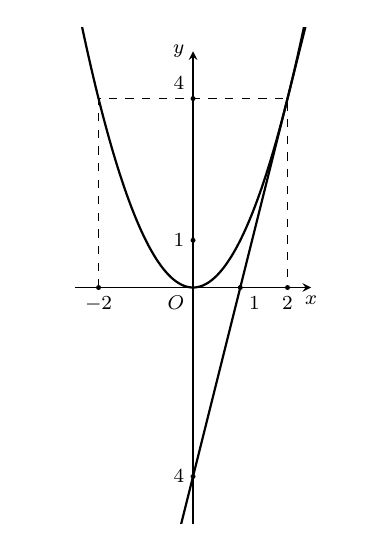
\begin{tikzpicture}[>=stealth,x=1cm,y=1cm,font=\footnotesize,scale=0.6]
					\def\a{1}
					\draw[->] (-2.5,0) -- (2.5,0) node[below] {$x$};
					\draw[->] (0,-5) -- (0,5) node[left] {$y$};
					\draw (0,0)node[below left]{$O$};
					\fill (-2,0)node[below]{$-2$} circle(1.5pt);
					\fill (1,0)node[below right]{$1$} circle(1.5pt);
					\fill (2,0)node[below]{$2$} circle(1.5pt);
					\fill (0,1)node[left]{$1$} circle(1.5pt);
					\fill (0,-4)node[left]{$4$} circle(1.5pt);
					\fill (0,4)node[above left]{$4$} circle(1.5pt);
					\clip (-3.5,-5)rectangle(3.5,5.5);
					\draw[thick,samples=150,smooth,domain=-3.5:3.5] plot(\x,{\a*(\x)^2});
					\draw[thick,samples=150,smooth,domain=-0.5:3.5] plot(\x,{4*\x-4});
					\draw[dashed] (-2,0)--(-2,4)--(2,4)--(2,0);
			\end{tikzpicture}}
		\end{enumerate}
	}
\end{bt}

% từ: cau-hoi/lop10/0D3_Ham_so_bac_hai_va_do_thi/0D3-1-5_Tinh_dong_bien_nghich_bien.tex
\begin{ex}%[0D3N1-5]%[ma:1d2cc019]
	Hàm số $y=(2m+1)x+m-3$ đồng biến  trên $\mathbb{R}$ khi
	\choice 
		{\True  $m >-\dfrac{1}{2}$}
		{$m\ge-\dfrac{1}{2}$} 
		{$m  <-\dfrac{1}{2}$}
		{$m  >\dfrac{1}{2}$}
	 \loigiai{
	Hàm số đã  cho đồng biến trên $\mathbb{R} \Leftrightarrow 2m+1 > 0\Leftrightarrow m >-\dfrac{1}{2}$.}
\end{ex}

% từ: cau-hoi/lop10/0D3_Ham_so_bac_hai_va_do_thi/0D3-1-5_Tinh_dong_bien_nghich_bien.tex
\begin{bt}%[0D3H1-5]%[Dự án đề kiểm tra Toán 10 GHKI NH23-24- Đào Hoàng Vũ]%[THPT Bùi Thị Xuân ]%[ma:50d0b963]
	Xét tính đồng biến, nghịch biến của hàm số $f(x)=x^2+2x+3$ trên khoảng $\left(-\infty;-1\right)$.
	\loigiai{
		Lấy $x_1$,  $x_2$ là 2 số tùy ý trên $\left(-\infty; -1\right)$ sao cho $x_1\neq x_2$.\\
		$\begin{aligned}
			\text{Xét} \ \dfrac{f(x_1)-f(x_2)}{x_1-x_2}&=\dfrac{x_1^2+2x_1+3-x_2^2-2x_2-3}{x_1-x_2}\\
			&=\dfrac{(x_1-x_2)(x_1+x_2)+2(x_1-x_2)}{x_1-x_2}\\
			&=\dfrac{(x_1-x_2)(x_1+x_2+2)}{x_1-x_2}\\
			&=x_1+x_2+2
		\end{aligned}$\\
		Do $x_1$, $x_2 \in\left(-\infty; -1\right)$ nên $x_1+x_2<-2$ hay $x_1+x_2+2<0$.\\
		Vậy hàm số nghịch biến trên khoảng $\left(-\infty; -1\right)$.
	}
\end{bt}

% từ: cau-hoi/lop10/0D3_Ham_so_bac_hai_va_do_thi/0D3-1-5_Tinh_dong_bien_nghich_bien.tex
\begin{bt}%[0D3H1-5]%[Mui Doan]%[ma:60e68bdc]
	Cho hàm số $ y=\dfrac{1}{x} $. Chứng tỏ hàm số đã cho 
	\begin{enumerate}
		\item Nghịch biến trên khoảng $ (0;+\infty) $.
		\item Nghịch biến trên khoảng $ (-\infty;0) $.
	\end{enumerate}
	\loigiai{
		\begin{enumerate}
			\item Nghịch biến trên khoảng $ (0;+\infty) $.\\
			Xét hai số bất kỳ $ x_1, x_2\in (0;+\infty) $ sao cho $ x_1<x_2 $.\\
			Ta có $ 0<x_1<x_2 $ nên $ \dfrac{1}{x_1}>\dfrac{1}{x_2}\Leftrightarrow  f(x_1)>f(x_2)$.\\
			Vậy hàm số nghịch biến trên $ (0;+\infty) $.
			\item Nghịch biến trên khoảng $ (-\infty;0) $.\\
			Xét hai số bất kỳ $ x_1, x_2\in (-\infty;0) $ sao cho $ x_1<x_2 $.\\
			Ta có $x_1<x_2<0 $ nên $ \dfrac{1}{x_1}>\dfrac{1}{x_2}\Leftrightarrow  f(x_1)>f(x_2)$.\\
			Vậy hàm số nghịch biến trên $ (-\infty;0) $.
		\end{enumerate}
	}
	
\end{bt}

% từ: cau-hoi/lop10/0D3_Ham_so_bac_hai_va_do_thi/0D3-1-5_Tinh_dong_bien_nghich_bien.tex
\begin{bt}%[0D3H1-5]%[Mui Doan]%[ma:7d22aac6]
	Cho hàm số $ y=f(x) $ có đồ thị như Hình $ 9 $.
	\immini{
		Chỉ ra khoảng đồng biến và khoảng nghịch biến của hàm số $ y=f(x) $.
	}
	{
		\begin{tikzpicture}[scale=0.7,>=stealth, font=\footnotesize, line join=round, line cap=round]
			\def\a{1} \def\b{1}  % Hệ số
			\def\c{2} \def\d{2}  % Hệ số
			\def\e{-1} \def\f{2}  % Hệ số
			\def\xmin{-4} \def\xmax{4.5}
			\def\ymin{-2.5} \def\ymax{3.5}
		%	\draw[opacity=0.3,gray] (-3,-2) grid (4,3);
			\draw[->] (\xmin,0)--(\xmax,0) node [below]{$x$};
			\draw[->] (0,\ymin)--(0,\ymax) node [left]{$y$};
			\draw 
			(-2,0) node[below ]{$ -2 $} 
			(-1,0) node[below ]{$ -1 $} 
			(1,0) node[below ]{$ 1 $} 
			(2,0) node[below ]{$2 $} 
			(3,0) node[below ]{$ 3 $} 
			(4,0) node[below ]{$ 4 $} 
			(0,1) node[left ]{$ 1 $} 
			(0,-1) node[left ]{$- 1 $} 
			(0,-2) node[left ]{$ -2 $} 
			(0,2) node[left ]{$ 2 $} 
			;
			\foreach \diemx/\diemy in {-2/0,-1/0,1/0,2/0,3/0,4/0,0/1,0/-1,0/-2}{\fill (\diemx,\diemy)circle(1pt);}
			\node at (0,0) [below right]{$O$};
			\node at (2.3,1.2) [above]{$y=f(x)$};
			\node[below] at (current bounding box.south){\it Hình $8$};  
			\clip (\xmin+0.1,\ymin+0.1) rectangle (\xmax-0.5,\ymax-0.1);
			\draw[smooth,samples=300] plot[domain=-3:-1](\x,{\a*(\x)+\b)});
			\draw[smooth,samples=300] plot[domain=-1:0](\x,{\c*(\x)+\d)});
			\draw[smooth,samples=300] plot[domain=0:2](\x,{\e*(\x)+\f)});
			\fill (0,0) circle(1pt);
			\node[below] at (current bounding box.south){\it Hình $8$};  
		\end{tikzpicture}
		
	}
	\loigiai{
		\begin{itemize}
			\item Hàm số đồng biến trên $ (-3:0) $ vì đồ thị hàm số  \lq\lq đi lên\rq\rq\, trên $ (-3;0) $.
			\item Hàm số nghịch biến trên $ (0;2) $ vì đồ thị hàm số  \lq\lq đi xuống\rq\rq\, trên $ (0;2) $.
		\end{itemize}	
	}
	
\end{bt}

% từ: cau-hoi/lop10/0D3_Ham_so_bac_hai_va_do_thi/0D3-1-5_Tinh_dong_bien_nghich_bien.tex
\begin{bt}%[0D3H1-5][1 điểm]%[Dự án đề kiểm tra HK1 22-23-Nhật Thiện]%[Trường Tân Bình]%[ma:59679cb5]
Xét tính đồng biến và nghịch biến của hàm số $f(x)=\dfrac{2}{x-3}$ trên khoảng $(3;+\infty)$.
\loigiai{
Tập xác định $\mathscr{D}=\mathbb{R}\setminus \{3\}$.\\
Lấy tùy ý $x_1,x_2 \in (3;+\infty)$ sao cho $x_1<x_2$, ta có
\begin{center}
	$x_1<x_2\Rightarrow x_1-3<x_2-3\Rightarrow \dfrac{2}{x_1-3}>\dfrac{2}{x_2-3}\Rightarrow f(x_1)>f(x_2)$.
\end{center}
Vậy hàm số nghịch biến trên khoảng $(3;+\infty)$.
}
\end{bt}

% từ: cau-hoi/lop10/0D3_Ham_so_bac_hai_va_do_thi/0D3-1-5_Tinh_dong_bien_nghich_bien.tex
\begin{bt}%[0D3N1-5]%[Dự án đề kiểm tra HKII NH22-23- Nguyễn Cường]%[THPT Trưng Vương]%[ma:66e7da22]
	Cho hàm số xác định trên $[-1;8]$ và có đồ thị như hình vẽ. Tìm tập giá trị, khoảng đồng biến, nghịch biến của hàm số.
	\begin{center}
		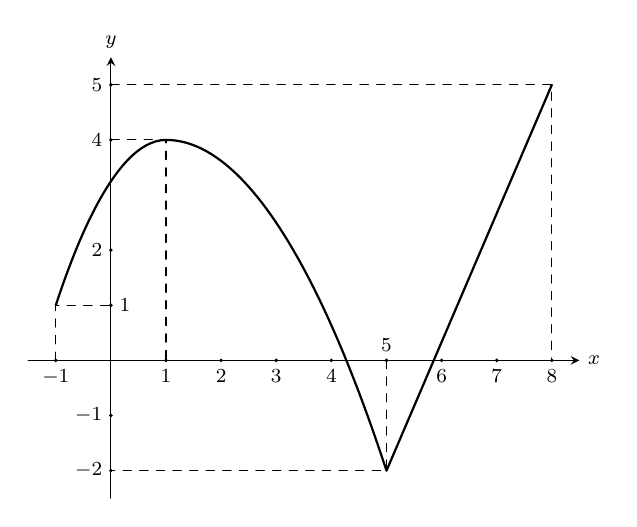
\begin{tikzpicture}[font=\footnotesize, line cap=round, line join =round, >=stealth, scale= .7]
			\def\xmin{-1}
			\def\xmax{8}
			\def\ymin{-2}
			\def\ymax{5}
			\draw[-stealth] (\xmin-.5,0)--(\xmax+.5,0)node[right]{$x$};
			\draw[-stealth] (0,\ymin-.5)--(0,\ymax+.5)node[above]{$y$};
%			\draw[thick,smooth, samples=200] plot[domain=-1:5] (\x,{(-1/2*(\x)^2+(3/2)*(\x)+3)});
			\draw[thick,smooth, samples=200] (-1,1) parabola bend (1,4) (5,-2);
			\draw[thick] (5,-2)--(8,5);
			\foreach \x in {-1,1,2,3,4,6,7,8}
			\fill[black] (\x,0) circle (1pt)node[below]{$\x$};
			\foreach \x in {5}
			\fill[black] (\x,0) circle (1pt)node[above]{$\x$};
			\foreach \y in {-2,-1,2,4,5}
			\fill[black] (0,\y) circle (1pt)node[left]{$\y$};
			\foreach \y in {1}
			\fill[black] (0,\y) circle (1pt)node[right]{$\y$};
			\draw[dashed]
			(-1,0)--(-1,1)--(0,1)
			(0,4)--(1,4)--(1,0)
			(5,0)--(5,-2)--(0,-2)
			(0,5)--(8,5)--(8,0)
			;
		\end{tikzpicture}
	\end{center}
\loigiai 
{
Hàm số đồng biến trên các khoảng $(-1;1)$, $(5;8)$ và nghịch biến trên khoảng $(1;5)$.\\
Tập giá trị của hàm số trên đoạn $[-1;8]$ là $[-2;5]$.
}
\end{bt}

% từ: cau-hoi/lop10/0D3_Ham_so_bac_hai_va_do_thi/0D3-2-1_Xac_dinh_ham_so_bac_hai.tex
\begin{ex}%[0D3Y2-1]%[ma:1dbf826f]
	Tung $ 1 $ đồng xu cân đối và đồng chất $  3 $ lần. Xác suất để có đúng $ 2 $ lần tung xuất hiện mặt $S$ là
	 \choice
		 {$\dfrac{1}{2}$}
		{$\dfrac{1}{4}$} 
		 {$\dfrac{3}{4}$}
		 {\True $\dfrac{3}{8}$}
	 \loigiai{
		Số phần tử  của không gian mẫu $ n\left(\Omega\right) =2^3=8$.\\
		Gọi $ A $ là biến  coos~\lq\lq có đúng $ 2 $ lần tung xuất hiện mặt sấp \rq\rq.\\
		Suy ra $ A=\{SSN; SNS;  NSS\} $.\\
		Do đó xác xuất cần tìm  là $ P(A)=\dfrac{3}{8} $.
	} 
\end{ex}

% từ: cau-hoi/lop10/0D3_Ham_so_bac_hai_va_do_thi/0D3-2-1_Xac_dinh_ham_so_bac_hai.tex
\begin{ex}%[0D3B2-1]%[ma:4fc3b8e2]
	Tung một đồng xu cân đối và đồng  chất ba lần liên tiếp. Tính xác suất để có ít nhất một lần tung xuất hiện mặt sấp.
	\choice 
		{\True  $\dfrac{7}{8}$}
		 {$\dfrac{1}{4}$}
		 {$\dfrac{1}{8}$}
		 {$\dfrac{3}{4}$}
	\loigiai{ 
		Số phần tử của  không gian mẫu $ n\left(\Omega\right) =2^3=8$.\\
		Gọi $ A $ là biến cố~\lq\lq có ít nhất một  lần tung xuất hiện mặt sấp \rq\rq.\\
		Suy ra $ \overline{A}$ \lq\lq không có lần nào xuất hiện mặt sấp, suy ra  $ \overline{A} =\{NNN\} $ và $ n\left(\overline A\right) =1$.\\
		Do đó xác xuất cần tìm  là $ P(A)=1-P(\overline{A})=\dfrac{7}{8} $.
	} 
\end{ex}

% từ: cau-hoi/lop10/0D3_Ham_so_bac_hai_va_do_thi/0D3-2-2_Bang_bien_thien_tinh_don_dieu_max_min.tex
\begin{bt}%[0D3H2-2]%[ma:729965ba]
	Tìm tập xác định và tập giá trị của các hàm số bậc hai sau:
	\begin{listEX}[2]
		\item $f(x)=-x^2+4 x-3$;
		\item $f(x)=x^2-7 x+12$.
	\end{listEX}
	\loigiai
	{
		\begin{enumerate}
			\item Tập xác định $\mathscr{D}=\mathbb{R}$. Tập giá trị là $(-\infty; 1]$.
			\item Tập xác định $\mathscr{D}=\mathbb{R}$. Tập giá trị là $\left[-\dfrac{1}{4};+\infty\right)$.			
		\end{enumerate}
	}
\end{bt}

% từ: cau-hoi/lop10/0D7_Bat_phuong_trinh_bac_2_mot_an/0D7-1-2_Dau_cua_tam_thuc_bac_2_va_ung_dung.tex
\begin{ex}%[0D7N1-2]%[ma:05919c4a]
	Tập nghiệm của bất phương trình $x^2-4  x+4>0$ là
	\choice 
		{\True $\mathbb{R} \setminus\{2\}$} 
		{$\mathbb{R}$} 
		{$(2;+\infty)$} 
		{$\mathbb{R} \setminus\{-2\}$} 
	\loigiai{ 
	Tam thức bậc hai $f(x)=x^2-4x+4$ có hệ số $a>0$ và nghiệm kép $x=2$ nên \break $x^2-4 x+4>0$, $\forall  x \neq 2$.}
\end{ex}

% từ: cau-hoi/lop10/0D7_Bat_phuong_trinh_bac_2_mot_an/0D7-2-1_Bat_phuong_trinh_bac_2_va_ung_dung.tex
\begin{ex}%[0D7H2-1]%[ma:2d579be5]
	Tìm tập  nghiệm $S$ của bất phương trình $-2x^{2}-3x+2>0$?\\
	\choice 
		{$S=\left(-\infty;-\dfrac{1}{2}\right)\cup(2;+\infty)$} 
		{$S=(-\infty;-2)\cup\left(\dfrac{1}{2};+\infty\right)$} 
		{\True $S=\left(-2;\dfrac{1}{2}\right)$} 
		{$S=\left(-\dfrac{1}{2};2\right)$} 
	 \loigiai{
		Ta  có $-2x^{2}-3x+2>0\Leftrightarrow-2<x<\dfrac{1}{2}$.\\
	} 
\end{ex}

% từ: cau-hoi/lop10/0D7_Bat_phuong_trinh_bac_2_mot_an/0D7-2-6_Bai_toan_co_tham_so.tex
\begin{bt}%[0D7H2-6]%[ma:1db16654]
	Tìm các giá trị của tham số $m$ để tam thức bậc hai $x^2+(m+1)x+2m+3$ dương với mọi $x\in\mathbb{R}$.
	\loigiai{
		Ta có
		\allowdisplaybreaks
		$\begin{aligned}[t]
			&\quad x^2+(m+1)x+2m+3>0,\,\,\forall x\in\mathbb{R}\\
			&\Leftrightarrow \heva{&a=1>0\,\,\text{(luôn đúng)}\\&\Delta=(m+1)^2-4\cdot 1\cdot (2m+3)<0}\\
			&\Leftrightarrow m^2-6m-11<0\\
			&\Leftrightarrow 3-2\sqrt{5}<m<3+2\sqrt{5}.
		\end{aligned}$
	}
\end{bt}

% từ: cau-hoi/lop10/0D7_Bat_phuong_trinh_bac_2_mot_an/0D7-2-6_Bai_toan_co_tham_so.tex
\begin{bt}%[0D7H2-6]%[Dự án đề kiểm tra GHKII NH22-23- Hiếu Mai]%Câu 5%[ma:4edf1b9b]
	Cho tam thức bậc hai $f(x)=-x^2+2(m+1)x-4$. Tìm tham số $m$ để $f(x)<0$ với mọi $x \in \mathbb{R}$.
	\loigiai{
	Tam thức bậc hai $f(x)=-x^2+2(m+1)x-4$ có $a=-1$, $b'=m+1$, $c=-4$.\\
	$\Delta'= (m+1)^2-(-1)\cdot (-4)=m^2+2m-3$.\\
	Ta có
	\allowdisplaybreaks
	$\begin{aligned}[t]
	f(x)<0,\, \forall x \in \mathbb{R}
		  \Leftrightarrow & \heva{&a<0\\&\Delta'<0}\\
		  \Leftrightarrow & \heva{&-1<0\\ & m^2+2m-3<0}\\
		   \Leftrightarrow & -3<m<1.
	\end{aligned}$\\
Vậy $-3<m<1$ thỏa đề bài.
	}
\end{bt}

% từ: cau-hoi/lop10/0D7_Bat_phuong_trinh_bac_2_mot_an/0D7-3-5_Phuong_trinh_khac_quy_ve_phuong_trinh_bac_2.tex
\begin{bt}%[0D7V3-5]%[ma:7dba8da1]
	Gọi $S$ là tập hợp các giá trị  nguyên của tham số $m\in[3;5]$ để phương trình $(m-2)x^4-2(m+1)x^2-3=0$ có đúng hai nghiệm phân biệt. Tổng các phần tử của tập $S$ bằng bao nhiêu?
	 \shortans{12}
	\loigiai{ 
		Đặt $t=x^2$ ($t\ge0$). 
		Phương trình đã cho  trở thành $(m-2)t^2-2(m+1)t-3=0$ (*)
		\begin{itemize}
			 \item Nếu $m=2$: phương trình đã cho trở thành $-6x^2-3=0\Leftrightarrow x^2=-\dfrac{1}{2}$ (vô nghiệm).
			 \item Nếu $m\ne2$:
			Để phương trình ban đầu có đúng $2$ nghiệm phân biệt thì phương  trình (*) phải có một nghiệm kép dương hoặc có hai nghiệm trái dấu.
			\begin{itemize}
				\item Trường hợp 1: (*) có nghiệm kép  dương khi và chỉ khi\\
				 \[\heva{
				 &\Delta'=0\\
				&\dfrac{m+1}{m-2}>0} 
				 \Leftrightarrow\heva{
				&  m^2+5m-5=0\\
				&  \hoac{&m>2\\&m<-1}
				}\Leftrightarrow  m=\dfrac{-5-3\sqrt{5}}{2}\notin [3;5].\]
				\item Trường hợp 2: (*) có  hai nghiệm trái dấu $\Leftrightarrow -3(m-2)<0\Leftrightarrow m>2$.
			\end{itemize}
			Vậy $S=\{3;4;5\}$ nên tổng  các phần tử của tập $S$ là $12$.
		\end{itemize}
	} 
\end{bt}

% từ: cau-hoi/lop10/0D7_Bat_phuong_trinh_bac_2_mot_an/0D7-3-6_Toan_hinh_toan_thuc_te_ung_dung_phuong_trinh.tex
\begin{bt}%[0D7V3-6]%[ma:cb441d24]
	\immini[thm]{Một ngọn hải đăng đặt tại vị trí $A$ cách bờ biển một khoảng cách $AB=5$ km. Trên bờ biển có một cái kho ở vị trí $C$ cách $B$ một khoảng là $8$ km. Người canh hải đăng có thể chèo thuyền từ $A$ đến vị trí $M$ trên bờ biển với vận tốc $4$ km/h rồi đi bộ đến $C$ với vận tốc $5$ km/h như hình bên. Tính khoảng cách từ vị trí $B$ đến $M$, biết thời gian người đó đi từ $A$ đến $C$ là $ 150 $ phút. Làm tròn kết quả đến hàng phần trăm.}
{\begin{tikzpicture}[scale=0.7, font=\footnotesize, line join=round, line cap=round, >=stealth]
		\path 
		(0,4) coordinate (A)
		(0,0) coordinate (B)
		(7,0) coordinate (C)
		(3,0) coordinate (M)
			;
		\draw (B)--(A)node[left,midway]{$5$ km}--(M);
		\draw[shorten <= -0.5cm,shorten >= -0.5cm] (B)--(C);
		\draw[dashed] (B)--+(0,-0.5)(C)--+(0,-0.5);
		\draw[<->,dashed,yshift=-0.3cm] (0,0)--(7,0) node[below,midway]{$8$ km};
		\foreach \p/\g in {A/90,B/135,C/90,M/45}\fill[black] (\p) circle (1pt) +(\g:.5)node{$\p$};
\end{tikzpicture}}
\shortans{$ 2{,}47 $}
\loigiai{
	Gọi $BM=x$ (km) suy ra $MC=8-a$ (km), ($0<x<8$).\\
	Theo giả thiết ta có $AM=\sqrt{AB^2+BM^2}=\sqrt{5^2+x^2}$.\\
	Từ đó suy ra \begin{eqnarray*}
		&&\dfrac{\sqrt{5^2+x^2}}{4}+\dfrac{8-x}{5}=\dfrac{150}{60}=\dfrac{5}{2}\\
		&\Leftrightarrow & 5\sqrt{5^2+x^2}=4x+18\\
		&\Leftrightarrow & 25(25+x^2)=16x^2+144x+324\\
		&\Leftrightarrow & 9x^2-144x+301=0\\
		&\Leftrightarrow & x=\dfrac{25+5\sqrt{11}}{3} \ \text{hoặc}\ x=\dfrac{25-5\sqrt{11}}{3}.
	\end{eqnarray*}
	Mà $ 0<x<8 $ nên $ x=\dfrac{25-5\sqrt{11}}{3} \approx 2{,}47$ (km).	
} 
\end{bt}

% từ: cau-hoi/lop10/0D7_Bat_phuong_trinh_bac_2_mot_an/0D7-3-6_Toan_hinh_toan_thuc_te_ung_dung_phuong_trinh.tex
\begin{bt}%[0D7V3-6]%[ma:d3b192ad]
	\immini{Hai ô tô cùng xuất phát tại vị trí $A$ và vị trí $B$ cách nhau $100$\,km chạy về thành phố $T$. Vận tốc của hai ô tô chạy từ vị trí $A$ và vị trí $B$ lần lượt là $50$\,km/h và $45$\,km/h. Biết rằng tại thời điểm ô tô đi từ vị trí $A$ đến địa điểm $D$ cách thành phố $T$ $12$\,km thì ô tô đi từ vị trí $B$ đến địa điểm $C$ cách thành phố $T$ là $6$\,km. Hỏi thời điểm đó, hai ô tô đã di chuyển được bao nhiêu giờ? (Kết quả làm tròn đến hàng phần mười)}
	{\begin{tikzpicture}[scale=.7]
			\coordinate [label=above:$A$](A) at (0,0);
			\coordinate [label=above:$D$](D) at (7,0);
			\coordinate [label=above right:$T$](T) at (9,0);
			\coordinate [label=right:$C$](C) at (9,-1);
			\coordinate [label=below right:$B$](B) at (9,-6);
			\foreach \diem in {A,D,T,C,B}	\fill (\diem)circle(2.5pt);		
			\draw[smooth](A)--(T)--(B)--(A);
			\foreach \x/\y/\z in {A/T/B}{\draw pic[draw,angle radius=4mm]{right angle=\x--\y--\z};}
			\draw [->]($(A)+ (.5,.5)$)--($(A)+ (1.5,.5)$);
			\draw [->]($(B)+ (.5,.5)$)--($(B)+ (.5,1.5)$);
			\draw ($(A)! .5 ! (B)$) node[left]{$100$ km};
	\end{tikzpicture}}
	\shortans[]{$1{,}3$}
	\loigiai{
		Gọi $x$ (giờ) là thời gian ô tô đi từ vị trí $A$ đến địa điểm $D $ $(x>0)$. \\
		Vì hai ô tô xuất phát cùng một lúc nên thời gian ô tô đi từ vị trí $B$ đến địa điểm $C$ cũng là $x$ giờ.\\
		Do đó, quãng đường $AD$ và $BC$ lần lượt là $50 x$ (km) và $45 x$ (km).\\
		Suy ra khoảng cách từ vị trí $A$ và vị trí $B$ đến thành phố $T$ lần lượt là $50 x+12$ (km) và $45 x+6$ (km).\\
		Vì khoảng cách giữa hai vị trí $A$ và $B$ là $100$ (km) nên ta có phương trình
		\begin{align*}
		\sqrt{(50 x+14)^{2}+(45 x+6)^{2}}=100 &\Leftrightarrow 5050 x^{2}+1560 x+180=100000\\&\Leftrightarrow 5050 x^{2}+1560 x-9840=0\\&\Leftrightarrow \hoac{&x\approx 1{,}3\\&x\approx -1{,}7.}
		\end{align*}
		Vì $x>0$, ta nhận $x=1{,}3$.\\
		Vậy thời điểm ô  $1$ đi từ $A$ đến địa điểm $D$ và ô tô $2$ đi từ $B$ đến vị trí $C$, hai ô tô đã di chuyển được $1{,}3$ giờ.
	}
\end{bt}

% từ: cau-hoi/lop10/0D7_Bat_phuong_trinh_bac_2_mot_an/0D7-3-6_Toan_hinh_toan_thuc_te_ung_dung_phuong_trinh.tex
\begin{bt}%[0D7V3-6]%[ma:bfda5131]
\immini{Lúc $8$ giờ sáng, hai ô tô cùng xuất phát tại vị trí $A$ và vị trí $B$ cách nhau $100$ km chạy về thành phố $T$. Vận tốc của hai ô tô chạy từ vị trí $A$ và vị trí $B$ lần lượt là $55$ km/h và $45$ km/h. Biết rằng tại thời điểm ô tô đi từ vị trí $A$ đến địa điểm $D$ cách thành phố $T$ là $14$ km thì ô tô đi từ vị trí $B$ đến địa điểm $C$ cách thành phố $T$ là $6$ km. Hỏi thời điểm đó là mấy giờ (đơn vị giờ)?
}{ \begin{tikzpicture}[scale=1, line join=round, line cap=round, >=stealth]
			\tikzset{every node/.style={scale=1}}
 	\def\r{4}
	\path 	(0:0) coordinate (A)
			++(0:\r) coordinate (T)	
			++(-90:\r) coordinate (B)
			($(A)!3/4!(T)$) coordinate (D)
			($(B)!4/5!(T)$) coordinate (C)
			(A)++(0.5,0.5) coordinate (A1)
			(A)++(2,0.5) coordinate (A2)
			(B)++(0.5,0.5) coordinate (B1)
			(B)++(0.5,2) coordinate (B2);
	\draw (A)--(T)--(B) (A)--(B) node[midway, sloped, below]{$100$ km}
			pic[draw,angle radius=2mm]{right angle=A--T--B};
	\draw[->,thick,>=latex] (A1)--(A2);
	\draw[->,thick,>=latex] (B1)--(B2);
	\foreach \x/ \goc in {A/90,B/0,C/0,T/45,D/90} 
			\fill (\x) circle (1pt)
			($(\x)+(\goc:3mm)$) node {$\x$};	
	\end{tikzpicture}}

\shortans{$9{,}2$}
\loigiai{
Gọi $x$ (giờ) là thời gian ô tô đi từ vị trí $A$ đến địa điểm $D$, $(x>0)$.\\ 
Vì hai ô tô xuất phát cùng một lúc nên thời gian ô tô đi từ vị trí $B$ đến địa điểm $C$ cũng là $x$ giờ.\\
Do đó, quảng đường $AD$ và $BC$ lần lượt là $55x$ km và $45x$ km.\\
Suy ra khoảng cách từ vị trí $A$ và vị trí $B$ đến thành phố $T$ lần lượt là $55 x+14$ (km)
và $45 x+6$ (km).\\
Vì khoảng cách giữa hai vị trí $A$ và $B$ là $100$ km nên ta có phương trình
$$\sqrt{(55 x+14)^2+(45 x+6)^2}=100 \Rightarrow 5050 x^2+2080 x+232=10000 .$$
Giải phương trình này và kết hợp với điều kiện ${x>0}$, ta nhận ${x=\dfrac{6}{5}}$.\\
Vậy thời điểm ô tô đi từ vị trí $A$ đến địa điểm $D$ là
$$8+ \dfrac{6}{5}  =9{,}2 \text{ (giờ)}.$$
}
\end{bt}

% từ: cau-hoi/lop10/0D8_Dai_so_to_hop/0D8-3-2_Khai_trien_mot_nhi_thuc_Newton.tex
\begin{bt}%[0D8H3-2]%[Dự án đề kiểm tra HKII NH22-23-BCTuan]%[THPT Thực Hành Sài Gòn]%[ma:2b85e789]
	Khai triển và rút gọn biểu thức:
	$$A=(x+2y)^5+(x-2y)^5
	$$
	\loigiai{
Ta có 
\begin{eqnarray*}
	\left(x+2y\right)^5&=&\mathrm{C}_5^0x^5+\mathrm{C}_5^1x^4\left(2y\right)^1+\mathrm{C}_5^2x^3\left(2y\right)^2+\mathrm{C}_5^3x^2\left(2y\right)^3+\mathrm{C}_5^4x^1{\left(2y\right)^4}+\mathrm{C}_5^5\left(2y\right)^5\\
	&=&x^5+10x^4y+40x^3y^2+80x^2y^3+80x{y^4}+32y^5.
\end{eqnarray*}
và
	\begin{eqnarray*}
		\left(x-2y\right)^5&=&\mathrm{C}_5^0x^5+\mathrm{C}_5^1x^4\left(-2y\right)^1+\mathrm{C}_5^2x^3\left(-2y\right)^2+\mathrm{C}_5^3x^2\left(-2y\right)^3+\mathrm{C}_5^4x^1{\left(-2y\right)^4}+\mathrm{C}_5^5\left(-2y\right)^5\\
		&=&x^5-10x^4y+40x^3y^2-80x^2y^3+80xy^4-32y^5.
	\end{eqnarray*}
Vậy $A=2x^5+80x^3y^2+160xy^4$.
}
\end{bt}

% từ: cau-hoi/lop10/0H4_He_thuc_luong_trong_tam_giac/0H4-1-3_Bien_doi_rut_gon_bieu_thuc_luong_giac.tex
\begin{ex}%[0H4H1-3]%[ma:b77d6b43]
	Cho  $\triangle ABC$, hệ thức nào sau đây là đúng?
	\choice 
		{$\sin  (A+B)=\cos C$}
		{$\cos \left(\dfrac{A}{3} \right)=\sin \left(\dfrac{B+C}{3}  \right)$}
		 {$\sin (A+B+C.=1$}
		 {\True $\cos \left(\dfrac{A}{2} \right)=\sin \left(\dfrac{B+C}{2} \right)$}
	\loigiai{ 
		Ta  có $\sin \left(\dfrac{B+C}{2} \right)=\sin \left(\dfrac{180^\circ-A}{2} \right)=\sin \left(90^{\circ}-\dfrac{A}{2} \right)=\cos \left(\dfrac{A}{2} \right)$.
	} 
\end{ex}

% từ: cau-hoi/lop10/0H4_He_thuc_luong_trong_tam_giac/0H4-2-1_Bai_toan_chi_dung_dinh_ly_Sin_Cosin.tex
\begin{bt}%[0H4N2-1]%[Tex hóa SGK CD-CT,T7/22, Phạm Tiến Long]%[ma:f4082816]
	Tính độ dài các cạnh chưa biết trong các tam giác sau:
	\begin{center}
		\begin{tikzpicture}[scale=1, font=\footnotesize, line join=round, line cap=round, >=stealth]
			
			\path
			(0,0) coordinate (A)
			(1.5,2.5) coordinate (C)
			($(A)!10/9!65:(C)$) coordinate (B)
			;
			\foreach \x/\g in {A/270,B/180,C/90} \fill[black] (\x) circle (1pt)+(\g:0.3) node{$\x$};
			\draw (A)--(B)node[pos=.5,left]{$10 $ cm}
			(A)--(C)node[pos=.5,right]{$9 $ cm}
			(B)--(C)
			(0,1)node{$65^\circ$}
			(0,-1)node{a)}
			;
			\tkzMarkAngle[mark=,size =0.7](C,A,B)
		
\end{tikzpicture}
		\hspace{2cm}
		\begin{tikzpicture}[scale=1, font=\footnotesize, line join=round, line cap=round, >=stealth]
			\path
			(0,0) coordinate (N)
			(3,0) coordinate (P)
			($(N)!1!112:(P)$) coordinate (M)
			;
			\foreach \x/\g in {N/270,P/0,M/90} \fill[black] (\x) circle (1pt)+(\g:0.3) node{$\x$};
			\draw (N)--(P)node[pos=.5,below]{$22 $ cm}
			(N)--(M)--(P)
			(-0.5,2)node{$34^\circ$}
			(0.3,1)node{$112^\circ$}
			(1.5,-1)node{b)}
			;
			\tkzMarkAngle[mark=,size =0.7](N,M,P)
			\tkzMarkAngle[mark=,size =0.7](P,N,M)
			\tkzMarkAngle[mark=,size =0.6](P,N,M)
		
\end{tikzpicture}
	\end{center}
	\loigiai{
		\begin{enumerate}[a)]
			\item $BC^2=AB^2+AC^2-2 \cdot AB \cdot AC \cdot \cos 65^\circ=10^2+9^2-2 \cdot 10 \cdot 9 \cdot \cos 65^\circ \approx 104{,}929$\\
			$\Rightarrow BC \approx 10{,}24$ cm.
			\item Ta có $NP=22$ cm; $\widehat{P}=180^\circ-\left(112^\circ+34^\circ\right)=34^\circ$.\\
			Áp dụng định lí sin, ta có  $\dfrac{MP}{\sin N}=\dfrac{MN}{\sin P}=\dfrac{NP}{\sin M}$.\\
			Suy ra $MP=\dfrac{NP\sin N}{\sin M}=\dfrac{22 \cdot \sin 112^\circ}{\sin 34^\circ} \approx 36{,}48$ cm.\\
			$\widehat{M}=\widehat{P} \Rightarrow \triangle NMP$ cân $N \Rightarrow NM=NP=22$ cm.
		\end{enumerate}
	}
\end{bt}

% từ: cau-hoi/lop10/0H4_He_thuc_luong_trong_tam_giac/0H4-3-1_Giai_tam_giac.tex
\begin{ex}%[0H4V3-1]%[ma:21a0c25e]
	Cho tam  giác $ABC$ có $BC=12\sqrt{3}$; $A=120^{\circ}$; $B=45^{\circ}$.
	\choiceTF 
		{\True Độ dài  cạnh $AC=12\sqrt{2}$ và $AB=6(\sqrt{6}-\sqrt{2})$}
		{Diện tích tam giác $ABC$ bằng  $54-18\sqrt{3}$}
		{Độ dài đường trung tuyến kẻ từ đỉnh  $A$ của tam giác là $m_a=36(5-2\sqrt{3})$}
		 {\True Bán kính đường tròn nội tiếp tam giác $ABC$ là $r=9\sqrt{2}+3\sqrt{6}-18$}
	 \loigiai{
		\begin{itemchoice}
			\itemch  Xét tam giác $ABC$ có
			$\widehat{A}+\widehat{B}+\widehat{C}=180^{\circ}$ (định lí  tổng $3$ góc trong tam giác).\\
			Suy ra $\widehat{C}=180^{\circ}-\widehat{A}-\widehat{B}=180^{\circ}-120^{\circ}-45^{\circ}=15^{\circ}  $.\\
			Áp  dụng định lí sintrong tam giác $ABC$, ta có\\
			$\dfrac{BC}{\sin A}=\dfrac{AC}{\sin  B}\Rightarrow AC=\dfrac{BC\cdot\sin B}{\sin A} =\dfrac{12\sqrt{3}\cdot\sin 45^{\circ}}{\sin 120^{\circ}}=12\sqrt{2}$.\\
			 Vậy $AC=12\sqrt{2}$.\\
			Mà $\dfrac{BC}{\sin A}=\dfrac{AB}{\sin C}\Rightarrow AB=\dfrac{BC\cdot\sin  C}{\sin A} =\dfrac{12\sqrt{3}\cdot\sin 15^{\circ}}{\sin 120^{\circ}}=6\left(\sqrt{6}-\sqrt{2}\right)$.\\
			Vậy  $AB=6\left(\sqrt{6}-\sqrt{2}\right)$.
			\itemch Diện tích tam  giác $ABC$ là\\
			$S_{ABC}=\dfrac{1}{2}AC\cdot BC\cdot\sin C =\dfrac{1}{2}\cdot  12\sqrt{2}\cdot 12\sqrt{3}\cdot\sin 15^{\circ}=108-36\sqrt{3}$.\\
			 Vậy $S_{ABC}=108-36\sqrt{3}$.
			\itemch Do  $m_a^2=\dfrac{b^2+c^2}{2}-\dfrac{a^2}{4}=\dfrac{(12\sqrt{2})^2+36\left(\sqrt{6}-\sqrt{2}\right)^2}{2}-\dfrac{(12\sqrt{3})^2}{4}=36\left(5-2\sqrt{3}\right)$.\\ Suy ra $m_a=6\sqrt{5-2\sqrt{3}}$.
			\itemch Ta có $S=p\cdot  r\Rightarrow r=\dfrac{S}{p}=2\cdot\dfrac{108-36\sqrt{3}}{12\sqrt{3}+12\sqrt{2}+6\sqrt{6}-6\sqrt{2}}=9\sqrt{2}+3\sqrt{6}-18$.
		\end{itemchoice}
	 }
\end{ex}

% từ: cau-hoi/lop10/0H4_He_thuc_luong_trong_tam_giac/0H4-3-1_Giai_tam_giac.tex
\begin{bt}%[Dự án Bài giảng K10-11, Phan Quốc Trí]%[0H4H3-1]%[ma:b91e5702]
	Giải tam giác $ABC$, biết $AB = 75$ m, $AC = 100$ m và $\widehat{A} = 32^{\circ}$.
	\loigiai{
		Đặt $a = BC, b = AC, c = AB$. Ta cần tính cạnh $a$ và hai góc $\widehat{B}$ và $\widehat{C}$.\\
		Áp dụng định lí côs-in, ta có
		$$a^2 = b^2 + c^2 - 2bc\cos A = 75^2 + 100^2 - 2 \cdot 75 \cdot 100 \cdot \cos 32° \approx 2904{,}3.$$
		Suy ra $a \approx \sqrt{2904{,}3} \approx 53{,}9$ (m).\\
		Áp dụng hệ quả định lí côs-in, ta có
		$$\cos B = \dfrac{a^2 + c^2 - b^2}{2ac} \approx \dfrac{53{,}9^2 + 75^2 - 100^2}{2 \cdot 53{,}9 \cdot 75} \approx -0{,}182.$$
		Suy ra $\widehat{B} \approx 100°29'10''$, $\widehat{C} \approx 47°30'50''$.
	}
\end{bt}

% từ: cau-hoi/lop10/0H4_He_thuc_luong_trong_tam_giac/0H4-3-1_Giai_tam_giac.tex
\begin{bt}%[Dự án Bài giảng K10-11, Phan Quốc Trí]%[0H4H3-1]%[ma:21ea2bd2]
	Cho tam giác $ABC$ có $AB=5$, $BC=7$, $AC=9$.  Tính số đo góc $A$ của tam giác đó (làm tròn kết quả đến độ).
	\loigiai{
		Áp dụng định lí côs-in ta có
		\begin{align*}
			&BC^2=AB^2+AC^2-2AB \cdot AC \cos A  \\
			\Leftrightarrow~ & \cos A = \dfrac{AB^2+AC^2- BC^2}{2AB \cdot AC}  \\
			\Leftrightarrow~ & \cos A = \dfrac{5^2+9^2-7^2}{2 \cdot 5 \cdot 9} =  \dfrac{19}{30}\\
			\Rightarrow~& \widehat{A} \approx 51^\circ.
		\end{align*}

	}
\end{bt}

% từ: cau-hoi/lop10/0H4_He_thuc_luong_trong_tam_giac/0H4-3-1_Giai_tam_giac.tex
\begin{bt}%[0H4V3-1]%[Dự án đề kiểm tra HKI NH22-23- Hieu Phan]%[THPT NGUYỄN HỮU TIẾN]%[ma:ee6625cb]
    Cho tam giác $ABC$ có $b=8 \mathrm{\,cm}$, $c=5 \mathrm{\,cm}$ và $\widehat{A}=60^{\circ}$.
    \begin{listEX}
        \item Tính độ dài đường cao $h_a$ của tam giác $ABC$.
        \item Tính bán kính $R$ của đường tròn ngoại tiếp tam giác $ABC$.
    \end{listEX}
   \dapso{
    a) $h_a=\dfrac{20\sqrt{3}}{7} \mathrm{\,cm}$;\qquad
    b) $R=\dfrac{7\sqrt{3}}{3} \mathrm{\,cm}$.
}
\loigiai{
\begin{listEX}
    \item Ta có $ S_{\triangle ABC}= \dfrac{1}{2}\cdot b\cdot c\cdot \sin A=\dfrac{1}{2}\cdot 8\cdot 5\cdot \dfrac{\sqrt{3}}{2}=10\sqrt{3}$ $\mathrm{cm^2}$.\\
    Và $ a=\sqrt{8^2+5^2-2\cdot 8\cdot 5\cdot \dfrac{1}{2}} =7$.\\
    Mặt khác  $S_{\triangle ABC}= \dfrac{1}{2}\cdot a
    \cdot h_a  \Rightarrow h_a=\dfrac{2S}{a}=\dfrac{20\sqrt{3}}{7}$ cm.
    \item Ta có $ S=\dfrac{abc}{4R}\Rightarrow R=\dfrac{abc}{4S}=\dfrac{7\cdot 8\cdot 5}{4\cdot 10\sqrt{3}}=\dfrac{7\sqrt{3}}{3}$ cm.
\end{listEX}
}
 
\end{bt}

% từ: cau-hoi/lop10/0H4_He_thuc_luong_trong_tam_giac/0H4-3-1_Giai_tam_giac.tex
\begin{bt}%[0H4H3-1]%[Dự án đề kiểm tra HKII NH22-23 - Nguyên Huỳnh]%[THPT Tam Phú]%[ma:1f95324e]
	Cho tam giác $ABC$ biết $CA=8{,}2$ và $\widehat{C}=110^{\circ}, \widehat{B} = 25^{\circ}$. Tính độ dài cạnh $BC$ và diện tích tam giác $ABC$. \dapso{$BC \approx 13{,}7, \enskip S_{ABC} \approx 52{,}9 $}
	\loigiai{Do $\widehat A+\widehat B+\widehat C=180^\circ$ nên $\widehat A=45^\circ$.\\
		Áp dụng định lý sin ta có 
		$$\dfrac{BC}{\sin A}=\dfrac{CA}{\sin B}\Rightarrow BC=\dfrac{CA\cdot\sin A}{\sin B}\approx 13{,}72.$$
		Ta có $S_{ABC}=\dfrac{1}{2}CA\cdot CB\cdot\sin C\approx\dfrac{1}{2}8{,}2\cdot13{,}72 \cdot\sin 110^\circ\approx52{,}86$.
	}
\end{bt}

% từ: cau-hoi/lop10/0H5_Vecto_chua_xet_toa_do/0H5-2-6_Toan_thuc_te_ap_dung_tong_hieu_vecto.tex
\begin{bt}%[0H5V2-6]%Câu 6%[ma:05c9da10]
	\immini{Một máy bay đang bay từ hướng đông sang hướng tây với tốc độ $700$ km/h thì gặp luồng gió thổi từ hướng đông bắc sang hướng tây nam với tốc độ $40$ km/h (Hình vẽ). Máy bay bị thay đổi vận tốc sau khi gặp gió thổi. Tìm tốc độ mới của máy bay (làm tròn kết quả đến hàng đơn vị theo đơn vị km/h).
	}{
		\begin{tikzpicture}[scale=1, font=\footnotesize, line join=round, line cap=round, >=stealth]
			\tikzset{every node/.style={scale=0.9}}
			\tikzset{maybay/.pic={
					%Đuôi máy bay
					\def\D{  (-2,-.45)--(-2.36,.24)--(-2.2,.3)--(-1.35,-.25)--cycle
						;}
					\draw \D;
					\fill[brown!40!] \D;
					
					%Quạt máy bay
					\def\Q{  (.15,-.1)
						..controls +(-140:0.1) and +(140:0.1) .. (.2,-.35)--(.8,-.17)--(.7,.07)--cycle
						
						;}
					\draw \Q;
					\draw[xshift=.5cm] \Q;
					\fill[brown!40!,xshift=.5cm] \Q;
					%---------elip2
					\draw[rotate=-70,xshift=-.23cm,yshift=1.27cm] (.7,-.1) ellipse (.12cm and .07cm);
					
					%Thân máy bay
					\def\T{  (-2.1,-.5)
						..controls +(40:0) and +(-170:0.7) .. (2,.74)
						..controls +(-40:0) and +(170:0.3) .. (2.55,.7)
						..controls +(-150:0) and +(30:.65) .. (2.1,.3)
						..controls +(-150:0) and +(-18:1.25) .. (-2.1,-.6)
						..controls +(90:0) and +(-90:0) .. (-2.1,-.51)
						-- (-2.5,-.52)--cycle;
					}
					\draw \T;
					\fill[brown!70!] \T;
					%Cánh máy bay
					\def\C{  (.5,.05)
						..controls +(170:0) and +(-10:0) .. (-1.48,.12)
						..controls +(-80:0) and +(170:0.02) .. (-1.65,.3)
						..controls +(180:0) and +(0:0) .. (-1.77,.3)
						..controls +(-80:0) and +(110:0) .. (-1.64,.12)
						..controls +(-35:0) and +(145:0) .. (-.2,-.17)
						--cycle
						;}
					\draw \C;
					\fill[brown!40!] \C;
					%Quạt sau
					\fill[brown!40!] \Q;
					%----elip 1
					\draw[rotate=-70,xshift=-.4cm,yshift=.8cm] (.7,-.1) ellipse (.12cm and .07cm);
					%Ô cửa
					\draw (2.18,0.73)--(2.5,0.7)--(2.14,0.58)--cycle;
					\fill[brown!40!](2.18,0.73)--(2.51,0.71)--(2.14,0.57)--cycle;
			}}
			\coordinate (O) at (0,0);
			\coordinate (A) at (180:2);
			\coordinate (B) at (240:1);
			\draw [->](O)--(A) node[midway,above]{$700$ km/h};
			\draw [->](O)--(B) node[right]{$40$ km/h};
			\draw pic["$60^\circ$",draw,angle eccentricity=0.5,angle radius=0.8cm]{angle=A--O--B};
			\path (O) pic[shift={(0:1.2)},scale=.4,rotate=200,yscale=-1.4]{maybay};
		\end{tikzpicture}
	}
	
	\shortans[]{$721$}
	\loigiai{
		Giả sử vận tốc của máy bay theo hướng đông sang tây là $\overrightarrow v_1$, vận tốc của luồng gió theo hướng đông bắc sang tây nam là $\overrightarrow v_2$ và vận tốc mới của máy bay chính là $\overrightarrow v$ thỏa mãn $$\overrightarrow v=\overrightarrow v_1+\overrightarrow v_2.$$
		Ta cần tính độ dài vectơ $\overrightarrow v$.\\
		Theo bài ra ta có $|\overrightarrow v_1|=700$, $|\overrightarrow v_2|=40$, $(\overrightarrow v_1,\overrightarrow v_2)=60^\circ$.\\
		Biểu diễn bài toán như hình vẽ dưới đây:
		\begin{center}
			\begin{tikzpicture}[scale=1, font=\footnotesize, line join=round, line cap=round, >=stealth]
				\tikzset{every node/.style={scale=0.9}}
				\tikzset{maybay/.pic={
						%Đuôi máy bay
						\def\D{  (-2,-.45)--(-2.36,.24)--(-2.2,.3)--(-1.35,-.25)--cycle
							;}
						\draw \D;
						\fill[brown!40!] \D;
						
						%Quạt máy bay
						\def\Q{  (.15,-.1)
							..controls +(-140:0.1) and +(140:0.1) .. (.2,-.35)--(.8,-.17)--(.7,.07)--cycle
							
							;}
						\draw \Q;
						\draw[xshift=.5cm] \Q;
						\fill[brown!40!,xshift=.5cm] \Q;
						%---------elip2
						\draw[rotate=-70,xshift=-.23cm,yshift=1.27cm] (.7,-.1) ellipse (.12cm and .07cm);
						
						%Thân máy bay
						\def\T{  (-2.1,-.5)
							..controls +(40:0) and +(-170:0.7) .. (2,.74)
							..controls +(-40:0) and +(170:0.3) .. (2.55,.7)
							..controls +(-150:0) and +(30:.65) .. (2.1,.3)
							..controls +(-150:0) and +(-18:1.25) .. (-2.1,-.6)
							..controls +(90:0) and +(-90:0) .. (-2.1,-.51)
							-- (-2.5,-.52)--cycle;
						}
						\draw \T;
						\fill[brown!70!] \T;
						%Cánh máy bay
						\def\C{  (.5,.05)
							..controls +(170:0) and +(-10:0) .. (-1.48,.12)
							..controls +(-80:0) and +(170:0.02) .. (-1.65,.3)
							..controls +(180:0) and +(0:0) .. (-1.77,.3)
							..controls +(-80:0) and +(110:0) .. (-1.64,.12)
							..controls +(-35:0) and +(145:0) .. (-.2,-.17)
							--cycle
							;}
						\draw \C;
						\fill[brown!40!] \C;
						%Quạt sau
						\fill[brown!40!] \Q;
						%----elip 1
						\draw[rotate=-70,xshift=-.4cm,yshift=.8cm] (.7,-.1) ellipse (.12cm and .07cm);
						%Ô cửa
						\draw (2.18,0.73)--(2.5,0.7)--(2.14,0.58)--cycle;
						\fill[brown!40!](2.18,0.73)--(2.51,0.71)--(2.14,0.57)--cycle;
				}}
				\coordinate (A) at (0,0);
				\coordinate (B) at (0:4);
				\coordinate (D) at (240:2);
				\coordinate (C) at ($(B)+(D)-(A)$);
				\draw [->](B)--(A) node[midway,above]{$\overrightarrow v_1$};
				\draw [->](B)--(C) node[midway, right]{$\overrightarrow v_2$};
				\draw [->](B)--(D) node[midway, above]{$\overrightarrow v$};
				\draw (A)--(D)--(C);
				\path (B) pic[shift={(0:1.2)},scale=.4,rotate=200,yscale=-1.4]{maybay};
				\foreach \i/\g in {A/90,B/90,C/0,D/180}{\draw[fill=white](\i) circle (1.0pt) ($(\i)+(\g:3mm)$) node[scale=1]{$\i$};}
			\end{tikzpicture}
		\end{center}
		Khi đó ta có $ABCD$ là hình bình hành có $\widehat{ABC}=45^\circ$.\\
		Suy ra $\widehat{DAB}=180^\circ-60^\circ=120^\circ$; $AD=|\overrightarrow v_2|=40$, $AB=|\overrightarrow v_1|=700$.\\
		Ta cần tính độ dài đoạn thẳng $BD$, đây chính là độ dài vectơ $\overrightarrow v$.\\
		Áp dụng định lí sin trong tam giác ABD, ta có
		\allowdisplaybreaks
		\begin{eqnarray*}
			BD^2&=&AD^2+AB^2-2\cdot AD\cdot AB\cdot \cos A\\
			&=&40^2+700^2-2\cdot 40\cdot 700\cdot \cos 120^\circ\\
			&=&519\,600.
		\end{eqnarray*}
		Suy ra $BD\approx721$ (km/h).\\
		Vậy tốc độ mới của máy bay sau khi gặp gió thổi là $721$ km/h.
	}
\end{bt}

% từ: cau-hoi/lop10/0H5_Vecto_chua_xet_toa_do/0H5-3-2_Bien_doi_thu_gon_1_dang_thuc_vecto.tex
\begin{bt}%[0H5H3-2]%[Đề kiểm tra GK1 môn Toán 10 trường THPT Đoàn Thượng]%[Mui Doan, 10EX-GK1-2223]%[ma:dac69202]
Cho hình bình hành $ABCD$ tâm $O$. Gọi $P$, $Q$, $R$ lần lượt là trung điểm của $AB$, $BC$, $AD$. Lấy $8$ điểm trên là điểm đầu hoặc điểm cuối của các véc-tơ. Tìm số các véc-tơ khác véc-tơ không, bằng với véc-tơ $\overrightarrow{AR}$.
	\loigiai{
	\immini{
	Số các véc-tơ khác véc-tơ không, bằng với véc-tơ $\overrightarrow{AR}$ là $\overrightarrow{RD}$, $\overrightarrow{BQ}$, $\overrightarrow{QC}$, $\overrightarrow{PO}$.
	}	
{
\begin{tikzpicture}[font=\footnotesize, line join=round, line cap=round, >=stealth]
\path (0,0) coordinate (A)
(-2,-2) coordinate (B)
(5,0) coordinate (D)
($(B)+(D)-(A)$) coordinate (C)
($(A)!.5!(C)$) coordinate (O)
($(A)!.5!(B)$) coordinate (P)
($(B)!.5!(C)$) coordinate (Q)
($(A)!.5!(D)$) coordinate (R)
;

\draw (A)--(B)--(C)--(D)--cycle (A)--(C) (B)--(D)
;	
\foreach \t/\g in {A/120,B/180,C/0,D/0,O/90,P/180,Q/-90,R/90}{
	\draw[fill=white] (\t) circle (1pt) node[shift={(\g:7pt)},font=\scriptsize]{$ \t $};
}
\end{tikzpicture}
	}
	}
\end{bt}

% từ: cau-hoi/lop10/0H5_Vecto_chua_xet_toa_do/0H5-3-5_Phan_tich_1_vecto_theo_2_vecto_khong_cung_phu.tex
\begin{bt}%[0H5H3-5]%[Dự án đề kiểm tra HKII NH22-23- NGUYỄN NGỌC DŨNG]%[PHẠM PHÚ THỨ]%[ma:951e5609]
Cho tam giác $A B C$ vuông tại $B$ có $B A=6$, $B C=8$. Gọi $M$ là điểm thưộc cạnh $A C$ sao cho $M A=2 M C$. Tính tích vô hướng $\overrightarrow{M A} \cdot \overrightarrow{M C}$.\\
\dapso{ $\overrightarrow{M A} \cdot \overrightarrow{M C}=\dfrac{-200}{9}$}
\loigiai{
Ta có $AC=\sqrt{AB^2+BC^2}=10$.\\
Mặt khác
$\heva{&MA=2MC \\ &MA+MC=AC} \Leftrightarrow \heva{&MA-2MC=0\\&MA+MC=10} \Leftrightarrow \heva{&MA=\dfrac{20}{3} \\ &MC =\dfrac{10}{3}}$.\\
Vậy $\overrightarrow{MA} \cdot \overrightarrow{MC}=\left|\overrightarrow{MA}
\right| \cdot \left| \overrightarrow{MC} \right| \cdot \cos \left(\overrightarrow{MA},\overrightarrow{MC}\right) = \dfrac{20}{3} \cdot \dfrac{10}{3} \cdot \cos 180^\circ = \dfrac{-200}{9}$.
}
\end{bt}

% từ: cau-hoi/lop10/0H5_Vecto_chua_xet_toa_do/0H5-4-2_Tim_goc_nho_tich_vo_huong.tex
\begin{bt}%[0H5V4-2]%Câu $37$ a)[Mức độ 3] % KIEM_TRA%[ma:0a59687d]
	\begin{enumerate}
		\item Trong mặt phẳng tọa độ $Oxy$, cho tam giác $ABC$ có $A (-4;1)$, $B(2;4)$, $C(2;-2)$. Gọi $G $ là trọng tâm và $H$ là trực tâm của tam giác $ABC$. Tìm tọa độ điểm $M$ thỏa mãn $3\overrightarrow{MG}+\overrightarrow{MH}=\overrightarrow{0}$.
		\item Trong mặt phẳng tọa độ $Oxy$, cho tam giác $ABC$ có $A(5;4)$, $B(-1;1) $, $C(3;-2)$. $M $ là điểm lưu động trên đường thẳng $AB$. Tìm $M$ để $\left|\overrightarrow{MA}+\overrightarrow{MC}\right|$ đạt giá trị nhỏ nhất.
	\end{enumerate}
		\loigiai{
		\begin{enumerate}
			\item Trọng tâm $G(0;1)$.\\
			Gọi $H(x;y)$ là trực tâm của$ \triangle ABC$. Ta có $\heva{&AH \perp BC\\ &BH \perp AC}\Leftrightarrow\heva{&\overrightarrow{AH}\cdot \overrightarrow{BC}=0\\&\overrightarrow{BH }\cdot \overrightarrow{AC}=0}$. $\qquad (*)$\\
			Ta có $\overrightarrow{AH}=(x+4; y-1)$, $\overrightarrow{BC}=(0;-6)$,  $\overrightarrow{BH}=(x-2;y-4)$, $\overrightarrow{AC}=(6;-3)$. \\
			Nên $(*)\Leftrightarrow\heva{&-6(y-1)=0\\ & 6(x-2)-3(y-4)=0}\Leftrightarrow\heva{& y=1\\ & 2x-y=0}\Leftrightarrow\heva{& x=\dfrac{1}{2}\\ & y=1.}$\\
			Suy ra $H\left(\dfrac{1}{2};1\right)$.\\
			Gọi $M(a;b)$.\\
			Ta có $3\overrightarrow{MG}+\overrightarrow{MH}=\overrightarrow{0} \Leftrightarrow\heva{&-3a+\dfrac{1}{2}-a=0\\ & 3(1-b)+1-b=0}\Leftrightarrow\heva{& a=\dfrac{1}{8}\\ & b=1.}$\\
			Vậy$M\left(\dfrac{1}{8};1\right) $.\\
			\item Gọi $M(x;y)$, $\overrightarrow{AB}=(-6;-3)$, $\overrightarrow{AM}=(x-5;y-4) $.
			\\
			$M\in AB \Rightarrow$ Ba điểm $A$, $B$, $M$ thẳng hàng. $\Rightarrow\overrightarrow{AB} $ và $ \overrightarrow{AM}$ cùng phương.\\
			$ \Leftrightarrow\dfrac{x-5}{-6}=\dfrac{y-4}{-3}\Rightarrow x=2y-3$. $\qquad(1)$\\
		 Ta có $\overrightarrow{MA}=(5-x;4-y)$, $\overrightarrow{MC}=(3-x;-2-y) \Rightarrow\overrightarrow{MA}+\overrightarrow{MC}=(8-2x;2-2y)$.\\
		 $ \left|\overrightarrow{MA}+\overrightarrow{MC}\right|=\sqrt{(8-2x)^2+(2-2y)^2}$. $\qquad(2)$\\
		Thế $(1)$ vào $(2)$ ta được\\
		$\left|\overrightarrow{MA}+\overrightarrow{MC}\right|=\sqrt{(14 -4y)^2+(2-2y)^2}=\sqrt{ 20y^2- 120y+ 200}=\sqrt{20 \left[(y-3)^2+1\right]}\ge\sqrt{20}$.\\
		Suy ra $\left|\overrightarrow{MA}+\overrightarrow{MC}\right|_{\min}=\sqrt{20}\Leftrightarrow y- 3=0 \Leftrightarrow y=3\Rightarrow x=3$.\\
		Vậy$ \left|\overrightarrow{MA}+\overrightarrow{MC}\right|_{\min}=\sqrt{20} $ khi và chỉ khi  $M (3;3) $.\\
		\end{enumerate}	
		}
\end{bt}

% từ: cau-hoi/lop10/0H9_Phuong_phap_toa_do_trong_mat_phang/0H9-1-3_Toa_do_diem_va_vecto_tren_he_truc_Oxy.tex
\begin{ex}%[0H9H1-3]%[ma:c2313e59]
	Trong mặt phẳng $Oxy$, cho hình bình hành $ABCD$ biết $A(2; 1)$, $B(2;-1)$, $C(-2;-3)$. Tọa độ giao điểm hai đường chéo của hình bình hành  $ABCD$ là
	\choice 
		 {$(2; 0)$}
		 {$(2; 2)$}
		{$(0;-2)$} 
		{\True $(0;-1)$} 
	\loigiai{ 
		Giao điểm hai đường chéo $ I $ là trung điểm  của $A C$.
		$$ 
		\heva{&x_I = \dfrac{x_A+x_B}{2}=0 \\ &y_I =  \dfrac{y_A+y_B}{2}=-1.}
		$$ 
		Vậy tọa độ giao điểm hai đường  chéo là $I(0;-1)$.
	} 
\end{ex}

% từ: cau-hoi/lop10/0H9_Phuong_phap_toa_do_trong_mat_phang/0H9-1-3_Toa_do_diem_va_vecto_tren_he_truc_Oxy.tex
\begin{bt}%[0H9H1-3]%[ma:482af04f]
	Cho tam giác $ABC$ có $M$, $N$, $P$ lần lượt là trung điểm của $BC$, $CA$, $AB$. Biết $M(1;1)$, $N(-2;-3)$, $P(2;-1)$. Tìm tọa độ các đỉnh của tam giác $ABC$.
	\loigiai{
		Ta có $\overrightarrow{MN}\left( -3;-4 \right)$, $\overrightarrow{PA}\left( {{x}_A}-2;{{y}_A}+1 \right)$, $\overrightarrow{MN}=\overrightarrow{PA}\Rightarrow A\left( -1;-5 \right)$.\\
		$N$ là trung điểm $AC$ suy ra $C\left( -3;-1 \right)$.\\ 
		$M$ là trung điểm $BC$ suy ra $B\left( 5;3 \right)$.
	}
\end{bt}

% từ: cau-hoi/lop10/0H9_Phuong_phap_toa_do_trong_mat_phang/0H9-2-2_Tim_goc_nho_tich_vo_huong.tex
\begin{bt}%[0H9B2-2]%[ma:aa8d60ff]
	Trong mặt phẳng tọa độ $Oxy$, cho điểm $N(-2;-3)$ và đường thẳng $d\colon-3x+5y+9=0$. Viết phương trình của đường thẳng $\Delta$ đi qua $N$ và $\Delta$ vuông góc với đường thẳng $d$. 
	 \loigiai{
		\begin{itemize}
			\item $d$ có véc-tơ  pháp tuyến $\overrightarrow{n}=(-3;5)$.
			\item Vì $\Delta\perp d$ nên $\Delta$ có véc-tơ pháp tuyến  $\overrightarrow{m}=(5;3)$.
			\item Phương trình của đường  thẳng $\Delta$ là
			 $$5(x+2)+3(y+3)=0\Leftrightarrow5x+3y+19=0.$$
		\end{itemize}
	 }
\end{bt}

% từ: cau-hoi/lop10/0H9_Phuong_phap_toa_do_trong_mat_phang/0H9-3-2_Phuong_trinh_duong_thang.tex
\begin{bt}%[0H9H3-2]%[Tex hóa SGK CD-CT,T7/22, Đoàn Minh Tân]%[ma:a561e25c]
	Trong mặt phẳng tọa độ $Oxy$, cho tam giác $MNP$ có $M(2;1)$, $N(-1;3)$, $P(4;2)$.
	\begin{enumerate}
		\item Tìm tọa độ của các véc-tơ $\overrightarrow{OM}$, $\overrightarrow{MN}$, $\overrightarrow{MP}$.
		\item Tích tích vô hướng $\overrightarrow{MN}\cdot \overrightarrow{MP}$.
		\item Tính độ dài các đoạn thẳng $MN$, $MP$.
		\item Tính $\cos\widehat{NMP}$.
		\item Tìm tọa độ trung điểm $I$ của $NP$ và trọng tâm $G$ của tam giác $MNP$.
	\end{enumerate}
	\loigiai{
		\begin{enumerate}
			\item Ta có $\overrightarrow{OM}=(2;1)$, $\overrightarrow{MN}=(-3;2)$, $\overrightarrow{MP}=(2;1)$.
			\item Ta có $\overrightarrow{MN}\cdot \overrightarrow{MP}=-3\cdot 2+2\cdot 1=-4$.
			\item Ta có $MN=\sqrt{(-3)^2+2^2}=\sqrt{13}$, $MP=\sqrt{2^2+1^2}=\sqrt{5}$.
			\item Ta có $\cos\widehat{NMP}=\dfrac{\overrightarrow{MN}\cdot\overrightarrow{MP}}{MN\cdot MP}=\dfrac{-4}{\sqrt{13}\cdot \sqrt{5}}=\dfrac{-4}{\sqrt{65}}$.
			\item $I$ là trung điểm của $NP$ nên $\heva{& x_I=\dfrac{-1+4}{2}=\dfrac{3}{2}\\ & y_I=\dfrac{3+2}{2}=\dfrac{5}{2}}\Rightarrow I\left(\dfrac{3}{2};\dfrac{5}{2}\right)$.\\
			$G$ là trọng tâm tam giác $MNP$ nên $\heva{ & x_G=\dfrac{2+(-1)+4}{3}=\dfrac{5}{3}\\ & y_I=\dfrac{1+3+2}{3}=2}\Rightarrow G\left(\dfrac{5}{3};2\right)$.
		\end{enumerate}
	}
\end{bt}

% từ: cau-hoi/lop10/0H9_Phuong_phap_toa_do_trong_mat_phang/0H9-3-8_Bai_toan_thuc_te_PP_toa_do_hoa.tex
\begin{bt}%[0H9H3-8]%[Tex hóa SGK CD,T93/104, Nguyễn Hoài Nam]%[ma:2da96a77]
	\immini{Quan sát hình bên và thực hiện các hoạt động sau
		\begin{enumerate}
			\item Lập phương trình đường thẳng $d$;
			\item Lập phương trình đường tròn $(C)$;
			\item Lập phương trình tiếp tuyến của đường tròn $(C)$ tại điểm $M\left(2+\sqrt{2};1+\sqrt{2}\right)$.
	\end{enumerate}}
	{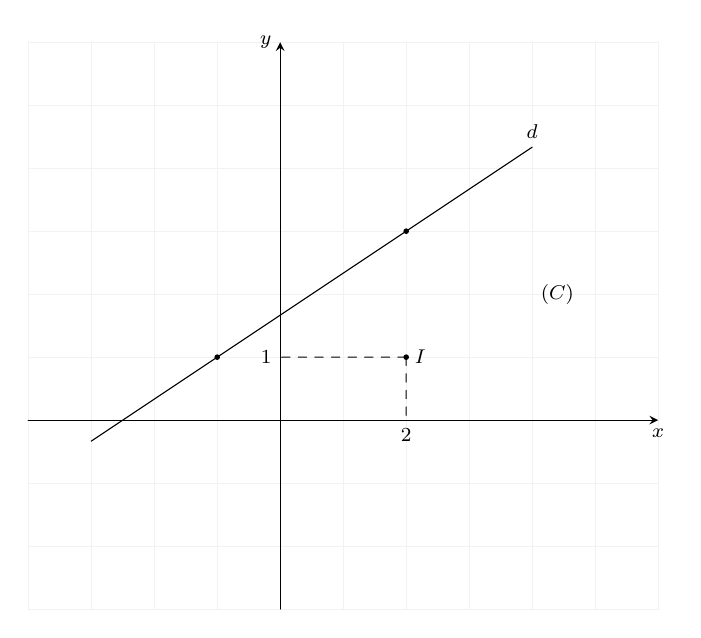
\begin{tikzpicture}[scale=0.8, font=\footnotesize, line join=round, line cap=round, >=stealth,
			declare function={
				f(\x)=\x*2/3+5/3;
			}
			]
			\draw[gray!10] (-4,-3) grid (6,6);
			\draw[->] (-4,0)--(6,0) node[below]{$x$};
			\draw[->] (0,-3)--(0,6) node[left]{$y$};
			
			\draw[smooth,black] plot[domain=-3:4] ({\x},{f(\x)}) node[above]{$d$};
			\draw[fill=black] (-1,1) circle (1pt);
			\draw[fill=black] (2,3) circle (1pt);
			\coordinate (I) at (2,1); 
			\coordinate (A) at (2,3); 
			\tkzDrawCircle(I,A)
			\draw[fill=black] (I) circle (1pt) node [right] {$I$};
			\draw[dashed] (I)--(0,1);
			\draw[dashed] (I)--(2,0);
			\draw[fill=black] (2,0) node [below] {$2$};
			\draw[fill=black] (0,1) node [left] {$1$};
			\draw[fill=black] (4,2) node [right] {$(C)$};
	\end{tikzpicture}}
	\loigiai{
		\begin{enumerate}
			\item Quan sát hình vẽ, ta thấy rằng đường thẳng $d$ đi qua hai điểm $A(-1;1)$ và $B(2;3)$.\\
			Ta có $\overrightarrow{AB} = (3;2) \Rightarrow \overrightarrow{n}_d = (2;-3)$.\\
			Phương trình đường thẳng $d$ là $2x-3y+5=0$.
			\item Đường tròn $(C)$ có tâm $I(2;1)$ và bán kính $R=2$.\\
			Phương trình đường tròn $(C)$ là $(x-2)^2 + (y-1)^2 = 4$.
			\item Gọi $\Delta$ là đường tiếp tuyến với $(C)$ tại $M$.\\
			Ta có $\overrightarrow{IM}=\left(\sqrt{2};\sqrt{2}\right) \Rightarrow \overrightarrow{n}_{\Delta} = (1;1)$.\\
			Phương trình tiếp tuyến $\Delta$ là $x+y-3-2\sqrt{2}=0$.
		\end{enumerate}
	}
\end{bt}

% từ: cau-hoi/lop10/0H9_Phuong_phap_toa_do_trong_mat_phang/0H9-4-2_Phuong_trinh_duong_tron.tex
\begin{ex}%[0H9Y4-2]%[ma:1d899392]
	\immini 
	 {
	Trong mặt  phẳng $Oxy$, đường tròn như hình bên có phương trình là một trong bốn phương trình sau. Hỏi đó là phương trình nào?
	\choice 
		{\True $(x-1)^2+(y+1)^2=4$} 
		{$(x+1)^2+(y-1)^2=2$} 
		{$(x+1)^2+(y-1)^2=4$} 
		 {$(x-1)^2+(y+1)^2=2$}
		 }
		{ 
		\begin{tikzpicture}[line join=round,line cap=round,>=stealth,thick,scale=0.8]
				 \draw[->] (-1.6,0)--(4,0) node[below left] {$x$};
				\draw[->]  (0,-3.5)--(0,2.5) node[below left] {$y$};
				\draw (0,0) node [below  left] {$O$};
				 \foreach \x in {-1,3}
				\draw[thin] (\x,1pt)--(\x,-1pt) node  [above] {$\x$};
				\foreach \y in  {-1,1,-3}
				 \draw[thin] (1pt,\y)--(-1pt,\y) node [left] {$\y$};
				\draw[dashed,thin](1,0) node[above]{$1$}--(1,-1)--(0,-1); 
				\coordinate  (I) at (1,-1);
				 \draw[name path=c] (I) circle (2 cm);
				\foreach \i in {I}{\draw  (\i) node[scale=0.9,below right]{$\i$};}
				\foreach \i  in {I}{\fill[black](\i) circle (0.8pt);}
				\draw[step=1,gray,dashed,thin] (-1.7,-3.6)  grid (4.2,2.6);
			\end{tikzpicture}
		 }
	 \loigiai{
		Từ hình vẽ ta thấy đường tròn có tâm $I(1; -1)$ và bán kính  $R=2$.\\
		Vậy phương trình  đường tròn là $(x-1)^2+(y+1)^2=4$.
	 }
\end{ex}

% từ: cau-hoi/lop10/0H9_Phuong_phap_toa_do_trong_mat_phang/0H9-4-7_Bai_toan_thuc_te_PP_toa_do_hoa.tex
\begin{bt}%[0H9V4-7]%[ma:1ea77dac]
	\immini[thm]{Hình vẽ bên mô phỏng một trạm thu phát sóng điện thoại di động đặt ở vị trí $I$ có tọa độ $(-2;1)$ trong mặt phẳng toạ độ (đơn vị trên hai trục là ki-lô-mét). Tính theo đường chim bay, xác định khoảng cách ngắn nhất để một người ở vị trí có tọa độ $(-3;4)$ di chuyển được tới vùng phủ sóng theo đơn vị
		ki-lô-mét (làm tròn kết quả đến hàng phần trăm). Biết rằng trạm thu phát sóng đó được thiết kế với bán kính phủ sóng $3$ km.
		}
	{
	\begin{tikzpicture}[line join=round, line cap=round,>=stealth,thick,scale=0.7]
		\def\xmax{2} \def\xmin{-6} \def\ymax{5} \def\ymin{-2}
		\def \R{3} % bán kính
		\draw[->] (\xmin,0) -- (\xmax,0)node[above]{\footnotesize  $x$};
		\draw[->] (0,\ymin) -- (0,\ymax) node[left] {\footnotesize  $y$};
		\draw (0,0)node[below right]{\footnotesize  $O$};\fill (0,0)circle(1.5pt);
		\foreach \x in{-2}
		\draw[shift={(\x,0)}] (0,-2pt)--(0,2pt)node[below=1pt]{\footnotesize $\x$};
		\foreach \y in{1}
		\draw[shift={(0,\y)}] (-2pt,0)--(2pt,0)node[right=1pt]{\footnotesize $\y$};
		\path (-2,1) coordinate (I) node[above] {\text{Trạm phát sóng}};
		\draw (I) circle (\R);
		\foreach \i/\x/\y/\g in{I/-2/1/-60}
		{\fill (\x,\y)circle(1.5pt) ($(\x,\y) + (\g:3mm)$)node{$\i$};   
			\draw[dashed,thin](\x,0)--(\x,\y)--(0,\y);}
	\end{tikzpicture}	
	}
	\shortans[]{$-6$}
	\loigiai{
		\begin{center}
			\begin{tikzpicture}[line join=round, line cap=round,>=stealth,thick,scale=0.8]
				\def\xmax{2} \def\xmin{-6} \def\ymax{5} \def\ymin{-2}
				\def \R{3} % bán kính
							\draw[->] (\xmin,0) -- (\xmax,0)node[above]{\footnotesize  $x$};
				\draw[->] (0,\ymin) -- (0,\ymax) node[left] {\footnotesize  $y$};
				\draw (0,0)node[below right]{\footnotesize  $O$};\fill (0,0)circle(1.5pt);
				\foreach \x in{-2}
				\draw[shift={(\x,0)}] (0,-2pt)--(0,2pt)node[below=1pt]{\footnotesize $\x$};
				\foreach \y in{4,1}
				\draw[shift={(0,\y)}] (-2pt,0)--(2pt,0)node[right=1pt]{\footnotesize $\y$};
				\coordinate (B) at (-3,4);
				\coordinate (I) at (-2,1);
				\path (-2,1) coordinate (I) node[above] {\text{Trạm phát sóng}};
				%\draw (I) circle (\R);
				\draw[name path=C,red] (I) circle (\R cm);
				\draw[name path=BI,dashed] (B)--(I);
				\path [name intersections={of=BI and C,by={M}}];
				%\clip (\xmin,\ymin)rectangle(\xmax,\ymax);
				\foreach \d/\g in {I/-80,B/90,M/-40} \draw[fill=white](\d)circle(1pt)+(\g:.4)node{\footnotesize $\d$};
				\foreach \x/\y in{-2/1,-3/4}\draw[dashed,thin](\x,0)--(\x,\y)--(0,\y);
			\end{tikzpicture}
		\end{center}
	Đường tròn màu đỏ mô tả ranh giới bên ngoài của vùng phủ sóng có tâm $I(-2;1)$ và bán kính phủ sóng $3$ km nên phương trình đường tròn đó là $(x+2)^2+(y-1)^2=9$.\\
	Giả sử vị trí đứng của người đó là $B(-3;4)$.\\
	Gọi $M$ (như trên hình vẽ) là giao điểm thứ nhất của đường tròn tâm $I$ và $BI$\\
	$\Rightarrow$ Khoảng cách ngắn nhất để người đó di chuyển được từ vị trí $B(-3;4)$ tới vùng phủ sóng là $BM$.\\
	Ta có $IB=\sqrt{(-3+2)^2+(4-1)^2}=\sqrt{10}$, suy ra $BM=IB-IM=\sqrt{10}-3=0{,}16$.
	}
\end{bt}

% từ: cau-hoi/lop11/1D1_Ham_so_luong_giac_va_phuong_trinh_luong/1D1-1-2_Chuyen_doi_don_vi_do_va_radian.tex
\begin{ex}%[1D1B1-2]%[ma:0468c355]
	Hàm số $y=\sqrt{3}+2\cos  x$ tăng trên khoảng
	\choice 
		 {$\left(-\dfrac{\pi}{6};\dfrac{\pi}{2}\right)$}
		{$\left(\dfrac{\pi}{2};\dfrac{3\pi}{2}\right)$} 
		{\True  $\left(\dfrac{7\pi}{6};2\pi\right)$}
		{$\left(\dfrac{\pi}{6};\dfrac{\pi}{2}\right)$} 
	\loigiai{ 
	\immini{ 
		Vì hàm số $y=\cos x$ đồng biến trên mỗi khoảng $\left(-\pi+k2\pi;k2\pi\right)$, $k\in\mathbb{Z}$ nên hàm số $y=\sqrt{3}+2\cos x$ cũng đồng biến trên  mỗi khoảng $\left(-\pi+k2\pi;k2\pi\right)$, $k\in\mathbb{Z}$.\\
		Vì  $\left(\dfrac{7\pi}{6};2\pi\right)\subset(\pi;2\pi)$ (với $k=1$) nên hàm số đồng biến trên khoảng $\left(\dfrac{7\pi}{6};2\pi\right)$.}
		{ 
		\begin{tikzpicture}[scale=.7,font=\footnotesize,line join=round,line cap=round,>=stealth]
				\def\r{3} \def\m{3.5} 
				\def\f (#1){(#1)} 
				\draw[->] (-\r,0)--(\r+0.5,0)  node[below] {$x$}node[above] {$\cos x$};
				\draw[->] (0,-\r)--(0,\r+0.5)  node[below right] {$y$} node[left]{$\sin x$};
				\draw (0,0)  node [below left] {$O$};
				 \foreach \x/\g/\z in {2.5/-45/1,-2.5/-135/-1}\fill[black] (\x,0) circle (1pt)+(\g:0.4) node{$\z$};
				\foreach \y/\g/\z in {2.5/135/1,-2.5/-135/-1}\fill[black] (0,\y) circle (1pt)+(\g:0.4) node{$\z$}; 
				\draw[color=white] (0,0)  circle (\r);
				\draw[-latex] (10:\r) arc  (10:70:\r);
				\draw (2.2,-0.2) node{$2\pi$} 
					(2.3,0.2) node{$0$} 
					 (.2,2.1) node{$\tfrac{\pi}{2}$}
					(-.2,-2.1)  node{$\tfrac{3\pi}{2}$}
					 (-2.3,0.2) node{$\pi$};
				\draw[-latex] (-10:\r)  arc (-10:-70:\r);
				\draw (0,0)  circle (2.5);
				\draw (2,3) circle  (6pt) node{$+$}
					(2,-3) circle (6pt) node{$-$}; 
			\end{tikzpicture}
		} 
	 }
\end{ex}

% từ: cau-hoi/lop11/1D1_Ham_so_luong_giac_va_phuong_trinh_luong/1D1-1-3_So_do_cua_mot_goc_luong_giac.tex
\begin{ex}%[1D1B1-3]%[ma:83971296]
	Trong các  hàm số được cho bởi các phương án sau đây, hàm số nào là hàm số chẵn?
	 \choice
		 {$y=\cot 2x$}
		{$y=\sin  2x$}
		{$y=\tan  2x$}
		{\True $y=\cos  2x$}
	\loigiai{ 
		Xét  hàm số $y=\cos 2x$ trên tập xác định $\mathscr{D}= \mathbb{R}$.\\
		Ta có $ \forall x\in \mathscr{D} \Rightarrow -x  \in \mathscr{D}$, ta có:
		$f(-x)= \cos \left({-2x}\right)=\cos 2x =f(x)$. \\ 
		Vậy hàm số $y=\cos 2x$ là hàm số  chẵn trên $ \mathbb{R}$.
	 }
\end{ex}

% từ: cau-hoi/lop11/1D1_Ham_so_luong_giac_va_phuong_trinh_luong/1D1-1-6_Toan_thuc_te_ap_dung_goc_luong_giac.tex
\begin{ex}%[1D1H1-6]%[ma:1e16d071]
	Khi xe đạp di chuyển, van $V$ của bánh xe quay quanh trục $O$ theo chiều kim đồng hồ với tốc độ góc không đổi là $11$ rad/s. Ban đầu van nằm ở vị trí $A$. Hỏi sau một phút di chuyển, khoảng cách từ van đến mặt đất là bao nhiêu, biết bán kính $OA=58$ cm? Giả sử độ  dày của lốp xe không đáng kể. (Kết quả làm tròn đến hàng phần mười).
	\begin{center}
		\begin{tikzpicture}[line join = round,line cap = round,scale = 1.3,transform shape]
				\clip (-3,-2.2) rectangle  (3.3,1.7);
				 \definecolor{beige}{rgb}{0.96,0.96,0.86}
				\definecolor{frenchblue}{rgb}{0.0,0.45,0.73} 
				 \definecolor{battleshipgrey}{rgb}{0.52,0.52,0.51}
				 \definecolor{earthyellow}{rgb}{0.88,0.66,0.37}
				\tikzset{xe_dap/.pic  = {
				 \draw[fill = battleshipgrey] (1.66,-.78) circle (31pt);
				\draw[fill = white]  (1.66,-.78) circle (26pt);
				\draw[fill = battleshipgrey] (-1.75,-.78) circle (31pt); 
				 \draw[fill = white] (-1.75,-.78) circle (26pt);
				 \draw[fill = battleshipgrey!40] (-.21,-1.02) circle (8pt);
				 \draw (-.21,-1.02) circle (6pt);
				\draw (-.21,-1.02)  circle (5pt);
				 \draw[fill = battleshipgrey] (-.21,-1.02) circle (2pt);
				\draw (-1.79,-.79)  circle (5pt);
				\draw (-1.79,-.79) circle  (4pt);
				\draw  (-1.77,-.94)--(-.3,-1.3)
					(-1.77,-.62)--(-.2,-.73); 
				\draw (-0.8,-.1)..controls +(120:1.05) and +(80:1.25)..(-2.95,-.7) 
					(0.45,-.65)..controls +(80:1.05) and  +(140:.5)..(2.2,.28)
					 (-1.2,.44)..controls +(110:.2) and +(-80:.28)..(-2.5,.65);
				\def\S{(-.91,1.07)--(-.72,.56)--(1.03,.72)--(.94,1.05)--(1.05,1.05) 
					..controls +(-75:.3)  and +(150:.2)..(1.68,-.76)--(1.6,-.82)
					..controls +(135:.3)  and +(-70:.2)..(1.05,.52)--(-.2,-1)--(-.27,-.9)--(.97,.6)--(-.7,.45)--(-.18,-1)--(-.315,-1)--(-.8,.4)--(-1.7,-.73
					 )--(-.35,-.9)--(-.31,-1)--(-1.87,-.8)--(-.85,.5)--(-1.05,1.07)--cycle}
				\draw[fill = frenchblue] \S; 
				 \fill[frenchblue] \S;
				 \def\Y{(-.5,1.2)
					..controls +(110:.08) and +(-10:.1)..(-1.2,1.32) 
					..controls +(-170:.4)  and +(-160:.4)..(-.85,1.1)
					 ..controls +(10:.1) and +(-60:.1)..(-.5,1.2)
				 }
				\draw[fill  = earthyellow] \Y;
				\fill[earthyellow]  \Y;
				\draw  (-1.7,-.79)--(-1.1,-1.44)
					(-1.8,-.86)--(-1.45,-1.65) 
					 (-1.74,-.86)--(-1.8,-1.7)
					(-1.8,-.86)--(-2.05,-1.65) 
					 (-1.74,-.86)--(-2.3,-1.5)
					 (-1.85,-.86)--(-2.5,-1.33)
					(-1.85,-.86)--(-2.65,-1) 
					(-1.85,-.75)--(-2.68,-.7) 
					 (-1.88,-.79)--(-2.55,-.35)
					 (-1.86,-.75)--(-2.2,0)
					(-1.75,-.7)--(-2.4,-0.13) 
					 (-1.8,-.7)--(-1.75,.15)
					 (-1.63,-.72)--(-1.05,-.17)
					(-1.5,-.75)--(-.9,-.44) 
					 (-1.77,-.85)--(-.93,-1.2); \draw (-1.75,-.7)--(-1.45,.5)
					 (-1.75,-.7)--(-2.2,.5);
				\draw[fill = battleshipgrey]  (-.14,-1)--(-.3,-1)--(-.25,-1.1)--(-.33,-1.5)--(-.45,-1.5)--(-.45,-1.6)..controls +(-15:.25) and +(-5:.25)..(-.25,-1.5)--(-.19,-1.1)--cycle;
				\draw[fill =  battleshipgrey] (-.23,-.72)--(-.18,-.5)--(-.3,-.5)--(-.28,-.4)--(0,-.4)..controls +(-5:.03) and +(-5:.2)..(-0.1,-.5)--(-.14,-.72)--cycle;
				\draw (1.72,-.78)--(2.52,-.5) 
					 (1.72,-.86)--(2.35,-.2)
					 (1.72,-.86)--(2.58,-.84)
					(1.72,-.8)--(2.48,-1.18) 
					 (1.6,-.86)--(2.3,-1.45)
					 (1.7,-.86)--(1.9,-1.65)
					 (1.6,-.86)--(1.6,-1.68)
					 (1.7,-.86)--(1.35,-1.63)
					 (1.6,-.76)--(1.05,-1.45)
					 (1.6,-.86)--(.9,-1.3)
					 (1.55,-.76)--(.77,-1)
					 (1.55,-.82)--(.74,-.7)
					(1.45,-.6)--(.83,-.38) 
					 (1.54,-.75)--(1,-.14)
					(1.63,-.74)--(1.55,.13) 
					 (1.63,-.74)--(2.1,0)
					(1.7,-.77)--(1.8,0.1); 
				 \draw[fill = black!70] (1.65,-.8) circle (2.3pt);
				 \draw (1.65,-.8) circle (5pt);
				\draw[fill = black!70] (-1.79,-.79) circle (2.3pt); 
				\draw[fill = earthyellow] (.92,1.06)..controls +(120:.15)  and +(-120:0)..(1.12,1.3)--(.85,1.45)--(.5,1.45)..controls +(120:.15) and +(-120:0)..(.5,1.58)--(.72,1.58)--(1.2,1.3)--(.7,1.6)--(.74,1.64)--(1,1.56)..controls +(-30:.5) and +(30:.3)..(1.05,1.06);
					 }}
				 \path
					 (0,0) pic[scale = 1]{xe_dap};
				 \def\xmin{0.5} \def\xmax{3.2}
				\def\ymin{-2.2} \def\ymax{.8} \draw[red,-  >] (\xmin,-.8)--(\xmax,-.8) node [above left]{\tiny $x$};
				\draw[red,- >] (1.65,\ymin)--(1.65,\ymax) node [left]{\tiny $y$}; 
				\draw[red](1.65,-.8)--(2.2,-1.5); 
				\node[red] at  (2.2,-1.5) [above]{\tiny $V$};
				\node[red] at (2.45,-.9) [above]{\tiny $A$}; 
				\node[red] at (1.65,-.8) [below left]{\tiny  $O$};
				\path  (2.5,-.9) coordinate (A)
					 (2.2,-1.5) coordinate (V)
					(1.65,-.8) coordinate  (O);
				\path (O) pic[draw,angle  radius = 0.4cm]{angle = V--O--A}node[shift = {(-22:19pt)}]{\footnotesize $\alpha$};
				 \draw[dashed] (1.65,-1.86)--(3,-1.86)
					 (1.65,-1.5)--(3,-1.5);
				\draw[red,< - >]  (2.8,-1.5)--(2.8,-1.86);
				 \node at (3,-1.8) [below left]{\tiny Mặt đất};
				\node at (2.8,-1.7)  [right]{\tiny?};
				 \path (current bounding box.south) node[below]{Hình 13};
			\end{tikzpicture}
	\end{center}
	\shortans{42,8} 
	 \loigiai{
		Sau một phút di chuyển, van $V$ quay được một góc là $-11\cdot 60=-660$ rad  do bánh xe quay cùng chiều kim đồng hồ nên tạo ra góc lượng giác có giá trị âm.\\
		Khi đó $l=58+58\cdot \sin  (-660) \approx 42{,}8$ cm.
	 }
\end{ex}

% từ: cau-hoi/lop11/1D1_Ham_so_luong_giac_va_phuong_trinh_luong/1D1-2-2_Xet_dau_gia_tri_luong_giac_Tinh_gia_tri_luong.tex
\begin{bt}%[1D1H2-2]%[ma:e9f737c2]
% nguon: Archive/SP_KhoLatex/ID6_old/1K1-1.tex #3727
%[Dự án 1 - TLDH - TeamTeXHoa - Đào Trung Kiên]
	Hoàn thành bảng sau
	\begin{center}
		\begin{tabular}{|l|c|c|c|c|c|c|}
			\hline Số đo độ & $15^{\circ}$ & $?$ & $0^{\circ}$ & $1900^{\circ}$ & $?$ & $?$ \\
			\hline $\begin{array}{c}\text { Số đo } \\
				\text { radian }\end{array}$ & $?$ & $\dfrac{3 \pi}{8}$ & $?$ & $?$ & $-\dfrac{7 \pi}{12}$ & $-\dfrac{11 \pi}{8}$ \\
			\hline
		\end{tabular}
		
	\end{center}\loigiai{
		Để hoàn thành bảng đã cho, ta thực hiện chuyển đổi từ độ sang rađian và từ rađian sang độ.
		Ta có \begin{eqnarray*}
			15^{\circ}&=&15 \cdot \dfrac{\pi}{180}=\dfrac{\pi}{12}\\
			0^{\circ}&=&0 \cdot \dfrac{\pi}{180}=0 \\
			900^{\circ}&=&900 \cdot \dfrac{\pi}{180}=5 \pi\\
			\dfrac{3 \pi}{8}&=&\dfrac{3 \pi}{8} \cdot\left(\dfrac{180}{\pi}\right)^{\circ}=67{,}5^{\circ} \\
			-\dfrac{7 \pi}{12}&=&-\dfrac{7 \pi}{12} \cdot\left(\dfrac{180}{\pi}\right)^{\circ}=-105^{\circ} \\
			-\dfrac{11 \pi}{8}&=&-\dfrac{11 \pi}{8} \cdot\left(\dfrac{180}{\pi}\right)^{\circ}=-247{,}5^{\circ}
		\end{eqnarray*}
		Vậy ta hoàn thành được bảng như sau
		\begin{center}
			\begin{tabular}{|l|c|c|c|c|c|c|}
				\hline Số đo độ & $15^{\circ}$ & $67{,}5^{\circ}$ & $0^{\circ}$ & $900^{\circ}$ & $-105^{\circ} $ & $-247{,}5^{\circ}$ \\
				\hline $\begin{array}{c}\text { Số đo } \\
					\text { radian }\end{array}$ & $\dfrac{\pi}{12}$ & $\dfrac{3 \pi}{8}$ & $0$ & $5\pi$ & $-\dfrac{7 \pi}{12}$ & $-\dfrac{11 \pi}{8}$ \\
				\hline
			\end{tabular}
		\end{center}
	}
\end{bt}

% từ: cau-hoi/lop11/1D1_Ham_so_luong_giac_va_phuong_trinh_luong/1D1-2-3_Bien_doi_rut_gon_bieu_thuc_luong_giac_chung_m.tex
\begin{ex}%[1D1H2-3]%[ma:df69ee64]
	Tính giá  trị của các biểu thức sau đây
	\begin{enumerate}
		\item $A=\sin ^25^{\circ}+\sin  ^210^{\circ}+\sin ^215^{\circ}+\cdots+\sin ^285^{\circ}$ (17 số hạng).
		\item $B=\cos 5^{\circ}+\cos 10^{\circ}+\cos 15^{\circ}+\cdots+\cos  175^{\circ}$ (35 số hạng)
	\end{enumerate}
	 \loigiai{
		\begin{enumerate}
			\item Vận dụng $\sin \left(90^{\circ}-\alpha \right)=\cos  \alpha$.\\
			 Ta có
			\begin{itemize}
				\item $\sin 85^{\circ}=\cos 5^{\circ}$. 
				\item  $\sin 80^{\circ}=\cos 10^{\circ}$.
				\item  $\sin 75^{\circ}=\cos 15^{\circ}$.
				\item  $\ldots$
				 \item $\sin 50^{\circ}=\cos 40^{\circ}$.
			\end{itemize}
			 Vậy
			\begin{align*}
				A&=\left(\sin ^25^{\circ}+\cos ^25^{\circ}  \right)+\left(\sin ^210^{\circ}+\cos ^210^{\circ} \right)+\cdots+\left(\sin ^240^{\circ}+\cos ^240^{\circ} \right)+\sin ^245^{\circ}\\
				&=\underbrace{1+1+\cdots+1}_{\text{8  số 1}}+\left(\dfrac{\sqrt{2}}{2} \right)^2=\dfrac{17}{2}.
			\end{align*}
			\item Vận  dụng $\cos \left(180^{\circ}-\alpha \right)=-\cos \alpha$.\\
			Ta  có
			\begin{itemize}
				\item $\cos 175^{\circ}=-\cos 5^{\circ}$. 
				\item $\cos 170^{\circ}=-\cos  10^{\circ}$.
				\item $\cos165^{\circ}=-\cos  15^{\circ}$.
				\item  $\ldots$
				\item $\cos 95^{\circ}=-\cos 85^{\circ}$. 
			\end{itemize}
			Vậy 
			\begin{align*}
				B&=\left(\cos 5^{\circ}+\cos  175^{\circ} \right)+\left(\cos 10^{\circ}+\cos 170^{\circ} \right)+\cdots+\left(\cos 85^{\circ}+\cos 95^{\circ} \right)+\cos 90^{\circ}\\
				 &=\underbrace{0+0+\cdots+0}_{\text{17 số 1}}+\cos 90^{\circ}=0.
			\end{align*}
	\end{enumerate}}
\end{ex}

% từ: cau-hoi/lop11/1D1_Ham_so_luong_giac_va_phuong_trinh_luong/1D1-2-4_Cac_goc_luong_giac_co_lien_quan_dac_biet_bu_n.tex
\begin{bt}%[1D1V2-4]%[ma:a5beffe9]
% nguon: Archive/2024/TOAN_11_XE/TOAN_11_XE/data4/11C1/KNTT-1.1.tex #1220

	Tính
	\begin{enumerate}
		\item $A=\sin^2 5^\circ+\sin^2 10^\circ+\sin^2 15^\circ+\ldots+\sin^2 85^\circ$ ($17$ số hạng);
		\item $B=\cos 5^\circ+\cos 10^\circ+\cos 15^\circ+\ldots+\cos 175^\circ$ ($35$ số hạng).
	\end{enumerate}
	\loigiai{
		\begin{enumerate}
			\item Nhận xét thấy $\sin^2 85^\circ=\left[\sin (90^\circ-5^\circ)\right]^2=\cos^2 5^\circ$.\\
			Do đó
			\begin{eqnarray*}
				A&=&\sin^2 5^\circ+\sin^2 10^\circ+\sin^2 15^\circ+\ldots+\sin^2 85^\circ\\
				&=&\sin^2 5^\circ+\sin^2 85^\circ+\sin^2 10^\circ+\sin^2 80^\circ+\ldots+\sin^2 45^\circ\\
				&=&\sin^2 5^\circ+\cos^2 5^\circ+\sin^2 10^\circ+\cos^2 10^\circ+\ldots+\sin^2 45^\circ\\
				&=&\underbrace {1+1+\ldots+1}_{8\text{ số hạng}}+\dfrac{1}{2}=\dfrac{17}{2}.
			\end{eqnarray*}
			\item Nhận xét thấy $\cos 175^\circ=\cos (180^\circ-5^\circ)=-\cos 5^\circ$.\\
			Do đó
			\begin{eqnarray*}
				B&=&\cos 5^\circ+\cos 10^\circ+\cos 15^\circ+\ldots+\cos 175^\circ\\
				&=&\cos 5^\circ+\cos 175^\circ+\cos 10^\circ+\cos 170^\circ+\ldots+\cos 90^\circ\\
				&=&\cos 5^\circ-\cos 5^\circ+\cos 10^\circ-\cos10^\circ+\ldots+\cos 90^\circ\\
				&=&\cos 90^\circ\\
				&=&0.
			\end{eqnarray*}
		\end{enumerate}
	}
\end{bt}

% từ: cau-hoi/lop11/1D1_Ham_so_luong_giac_va_phuong_trinh_luong/1D1-2-5_Toan_thuc_te_ap_dung_gia_tri_cua_mot_goc_luon.tex
\begin{ex}%[1D1H2-5]%[ma:d9028f45]
	 Xét tính đúng sai của các khẳng định sau.
	 \choiceTF
		 {$\sin x\cos ^5x-\cos x\sin ^5x=\sin 4x$}
		{$\dfrac{\sin 3x\cos  2x+\sin x\cos 6x}{\sin 4x}=\cos3x$;}
		{$\dfrac{\cos x-\cos 2x+\cos 3x}{\sin x-\sin 2x+\sin  3x}=\cot 2x$}
		{$\dfrac{2\sin \left(x+y\right)}{\cos \left(x+y\right)+\cos  \left(x-y\right)}-\tan y=1$}
	\loigiai{ 
		\begin{itemchoice}
			\itemch 
			\begin{eqnarray*}
				\sin  x\cos ^5x-\cos x\sin ^5x&=&\sin x\cos x\left(\cos ^4x-\sin ^4x\right)
				\\ 
				&=&\dfrac{1}{2} \sin 2x\left(\cos  ^2x-\sin ^2x\right)\left(\cos ^2x+\sin ^2x\right)\\
				&=&\dfrac{1}{2} \sin 2x\cos  2x=\dfrac{1}{4} \sin 4x.
			\end{eqnarray*}
			 \itemch Ta có
			\begin{eqnarray*}\dfrac{\sin 3x\cos 2x+\sin x\cos 6x}{\sin 4x}&=&\dfrac{\dfrac{1}{2} \left(\sin x+\sin 5x\right)+\dfrac{1}{2} \left[\sin \left(-5x\right)+\sin 7x\right]}{\sin 4x}\\
				&=&\dfrac{\sin x+\sin  5x-\sin 5x+\sin 7x}{2\sin 4x}\\
				&=&\dfrac{\sin x+\sin 7x}{2\sin 4x}\\ 
				 &=&\dfrac{2\sin 4x\cos 3x}{2\sin 4x}\\
				&=&\cos 3x. 
			\end{eqnarray*}
			\itemch 
			\begin{eqnarray*}\dfrac{\cos x-\cos 2x+\cos 3x}{\sin x-\sin 2x+\sin 3x}&=&\dfrac{\left(\cos x+\cos 3x\right)-\cos 2x}{\left(\sin x+\sin 3x\right)-\sin 2x}\\
				&=&\dfrac{2\cos 2x\cos x-\cos 2x}{2\sin 2x\cos  x-\sin 2x}\\
				&=&\dfrac{\cos 2x\left(2\cos x-1\right)}{\sin 2x\left(2\cos  x-1\right)}\\
				 &=&\dfrac{\cos 2x}{\sin 2x}=\cot 2x.
			\end{eqnarray*}
			\itemch 
			\begin{eqnarray*}
				\dfrac{2\sin \left(x+y\right)}{\cos \left(x+y\right)+\cos \left(x-y\right)}-\tan y&=&\dfrac{2\left(\sin x\cos y+\cos x\sin y\right)}{2\cos x\cos y}-\tan  y\\
				&=&\dfrac{\sin x}{\cos x}+\dfrac{\sin  y}{\cos y}-\tan y\\
				&=&\tan x+\tan y-\tan y=\tan  x.
			\end{eqnarray*}
		\end{itemchoice}
	} 
\end{ex}

% từ: cau-hoi/lop11/1D1_Ham_so_luong_giac_va_phuong_trinh_luong/1D1-3-2_Ap_dung_cong_thuc_cong.tex
\begin{bt}%[1D1V3-2]%[ma:7910f8f2]
% nguon: Archive/SP_KhoLatex/ID6_old/1K1-2-1.tex #3470
[VDT]%[DCHT Toán 11 - KNTT -Phong Lê] 
	Không sử dụng máy tính, hãy tính $P = \cos 20^{\circ}\cos 40^{\circ} - \sin 140^{\circ}\sin 160^{\circ}.$
	\dapso{$P = \dfrac{1}{2}$.}
	\loigiai{Ta có \\
		$P = \cos 20^{\circ}\cos 40^{\circ} - \sin 140^{\circ}\sin 160^{\circ} = \cos 20^{\circ}\cos 40^{\circ} -\sin 40^{\circ}\sin 20^{\circ} = \cos\left(40^{\circ}+20^{\circ}\right) = \cos 60^{\circ} = \dfrac{1}{2}$.\\
		Vậy $P= \dfrac{1}{2}$.
	}
\end{bt}

% từ: cau-hoi/lop11/1D1_Ham_so_luong_giac_va_phuong_trinh_luong/1D1-3-2_Ap_dung_cong_thuc_cong.tex
\begin{bt}%[1D1C3-2]%[ma:fa13ef14]
% nguon: Archive/SP_KhoLatex/ID6_old/1K1-2.tex #3612

	Cho tam giác $A B C$ có $\widehat{B}=75^{\circ}$; $\widehat{C}=45^{\circ}$ và $a=B C=12 \mathrm{~cm}$.
	\begin{enumerate}
		\item Sử dụng công thức $S=\dfrac{1}{2} a b \sin C$ và định lí sin, hãy chứng minh diện tích của tam giác $A B C$ cho bởi công thức $$S=\dfrac{a^2 \sin B \sin C}{2 \sin A}.$$
		\item Sử dụng kết quả ở câu a và công thức biến đổi tích thành tổng, hãy tính diện tích $S$ của tam giác $ABC$.
	\end{enumerate}
	\loigiai{
		\begin{enumerate}
			\item Định lí sin trong tam giác $A B C$ với $BC=a$, $AC=b$ và $A B=c$ là $$\dfrac{a}{\sin A}=\dfrac{b}{\sin B}=\dfrac{c}{\sin C}.$$
			Từ đó suy ra $b=\dfrac{a \sin B}{\sin A}$.\\
			Diện tích tam giác $ABC$ là $S=\dfrac{1}{2} a b \sin C=\dfrac{1}{2} a \cdot \dfrac{a \sin B}{\sin A} \cdot \sin C=\dfrac{a^2 \sin B \sin C}{2 \sin A}$.\\
			Vậy $S=\dfrac{a^2 \sin B \sin C}{2 \sin A}$ (Điều phải chứng minh).
			\item Ta có $\widehat{A}+\widehat{B}+\widehat{C}=180^{\circ}$ (định lí tổng ba góc trong tam giác $ABC$).\\
			$\Rightarrow \hat{A}=180^{\circ}-(\hat{B}+\hat{C})=180^{\circ}-\left(75^{\circ}+45^{\circ}\right)=60^{\circ}$.\\
			Ta có
			\begin{eqnarray*}
				S&=&\dfrac{a^2 \sin B \sin C}{2 \sin A}=\dfrac{12^2 \sin 75^{\circ} \sin 45^{\circ}}{2 \sin 60^{\circ}}
				=\dfrac{144 \cdot \dfrac{1}{2}\left[\cos \left(75^{\circ}-45^{\circ}\right)-\cos \left(75^{\circ}+45^{\circ}\right)\right]}{2 \cdot \dfrac{\sqrt{3}}{2}}\\
				&=&\dfrac{72\left(\cos 30^{\circ}-\cos 120^{\circ}\right)}{\sqrt{3}}=\dfrac{72\left[\dfrac{\sqrt{3}}{2}-\left(-\dfrac{1}{2}\right)\right]}{\sqrt{3}}=36+12 \sqrt{3}.
			\end{eqnarray*}
			Vậy diện tích của tam giác $ABC$ là $S=36+12 \sqrt{3}$ (đvdt).
		\end{enumerate}
	}
\end{bt}

% từ: cau-hoi/lop11/1D1_Ham_so_luong_giac_va_phuong_trinh_luong/1D1-3-5_Ket_hop_nhieu_cong_thuc_luong_giac.tex
\begin{ex}%[1D1V3-5]%[ma:7d01b9dc]
	Cho $3\cos \alpha-\sin \alpha=1$, với  $0^{\circ} < \alpha < 90^{\circ}$. Tính giá trị của $\tan \alpha$. (Kết quả làm tròn đến hàng phần mười).
	 \shortans{1,3}
	 \loigiai{
		 Ta có \allowdisplaybreaks
		\begin{eqnarray*}
			&&3\cos \alpha-\sin  \alpha=1\\
			&\Leftrightarrow& 3\cos  \alpha=\sin \alpha+1\\
			&\Rightarrow&  9\cos ^2\alpha=(\sin \alpha+1)^2\\
			 &\Leftrightarrow& 9\cos ^2\alpha=\sin ^2\alpha+2\sin \alpha+1\\
			&\Leftrightarrow& 9\left(1-\sin ^2\alpha\right)=\sin ^2\alpha+2\sin  \alpha+1\\
			&\Leftrightarrow&  10\sin ^2\alpha+2\sin \alpha-8=0\\
			&\Leftrightarrow& \hoac{&\sin  \alpha=-1\\
			&\sin  \alpha=\dfrac{4}{5}.}
		\end{eqnarray*}
		\begin{itemize}
			\item $\sin \alpha=-1$: không thỏa mãn vì $0^{\circ} < \alpha < 90^{\circ}$. 
			\item $\sin \alpha=\dfrac{4}{5} \Rightarrow \cos \alpha=\dfrac{3}{5} \Rightarrow \tan \alpha=\dfrac{\sin \alpha}{\cos \alpha}=\dfrac{4}{3}\approx 1{,}3$. 
		\end{itemize}
	 }
\end{ex}

% từ: cau-hoi/lop11/1D1_Ham_so_luong_giac_va_phuong_trinh_luong/1D1-4-6_Tim_tap_gia_tri_va_min_max.tex
\begin{ex}%[1D1V4-6]%[ma:66a05a4a]
	Tính giá trị lớn nhất của $E=2\sin \alpha-\sin  ^2\alpha+3$
	\choice 
		{$2$} 
		 {$3$}
		{\True  $4$}
		{$1$} 
	 \loigiai{
		$E=2\sin \alpha-\sin ^2\alpha+3=-(\sin  \alpha-1)^2+4$.\\
		Ta có \[ 
		\begin{aligned}
			&-1\leq  \sin \alpha \leq 1, \forall \alpha\in\mathbb{R}\\
			 &\Leftrightarrow-2\leq \sin \alpha-1\leq 0, \forall \alpha\in\mathbb{R}
			\\ 
			 &\Leftrightarrow 0\leq(\sin \alpha-1)^2\leq 4, \forall \alpha\in\mathbb{R}\\
			&\Leftrightarrow-4\leq-(\sin \alpha-1)^2\leq  0, \forall \alpha\in\mathbb{R}\\
			&\Leftrightarrow 0\leq E\leq  4, \forall \alpha\in\mathbb{R}.
		\end{aligned}
		 \]
		Dấu bằng xảy ra khi và chỉ khi 
		\allowdisplaybreaks 
		\begin{eqnarray*}
			E=4\Leftrightarrow \sin\alpha=1\Leftrightarrow  \alpha=\dfrac{\pi}{2}+k2\pi,k\in\mathbb{Z}.
		\end{eqnarray*}
		Vậy giá trị  lớn nhất của $E$ là $4$.
	 }
\end{ex}

% từ: cau-hoi/lop11/1D1_Ham_so_luong_giac_va_phuong_trinh_luong/1D1-4-8_Toan_thuc_te_ap_dung_ham_so_luong_giac.tex
\begin{bt}%[1D1V4-8]%[ma:53c9f10e]
% nguon: Archive/2025-Sangtac/Khoi11/Data/1-CTST/CTST_1-OTGK1_De05.tex #5004
%[Câu 1]
	Khi đu quay hoạt động, vận tốc theo phương ngang của một cabin $M$ phụ thuộc vào góc lượng giác $\alpha = (Ox, OM)$ theo hàm số $v_x = 0{,}25\sin\alpha$ (m/s). Vận tốc lớn nhất của cabin là
	\begin{center}
		\begin{tikzpicture}[scale=0.7,font=\small,line join=round,line cap=round,>=stealth]
			\tikzset{declare function={g=0;}}
			\coordinate (O) at (0,0);
			%	\coordinate[label=above right:$A$] (A) at (0:4.4);
			%	\coordinate[label=above right:$M$] (M) at (30+g:4.4);
			\pgfmathsetmacro{\gx}{60-g};
			\coordinate (v) at ($(M)+(120+g:3.3)$);
			\coordinate (vx) at ($(M)+(180:3.3*cos \gx)$);
			\draw[thick] (O) circle(4.4) (O) circle(3.53);
			\foreach \t in {0,1,...,11}{
				\draw[very thick,fill] (O)--(g+30*\t:4.4)circle(0.06);
				\begin{scope}[shift={(g+30*\t:4.4)}]
					\draw[fill=teal] (-0.27,0)--(0.27,0)--(0.36,-0.18)--(-0.36,-0.18)--cycle
					(0.32,-0.18)--(0.32,-0.54) (-0.32,-0.18)--(-0.32,-0.54)
					(-0.4,-0.54)--(0.4,-0.54)--(0.27,-1)--(-0.27,-1)--cycle;
			\end{scope}}
			\draw[fill=gray!70!yellow] (0.2,0)--(2.35,-5.53)--(3.65,-5.53)--(3.65,-6.02)--(1.95,-6.02)--(0,-0.85)--(-1.95,-6.02)--(-3.65,-6.02)--(-3.65,-5.53)--(-2.35,-5.53)--(-0.2,0)--cycle;
			\draw[fill=gray!10!yellow] (O) circle(0.34);
			\draw[fill] (-5,-5.85)--(0,-5.85) circle(0.08)--(6.4,-5.85);
			\draw[->] (-5,0)--(6.7,0) node [below]{\color{black}$x$};
			\path 
			(3.82,2.22) coordinate (M)
			($(M)-(1.8,0)$) coordinate (N)
			($(N)+(0,2.5)$) coordinate (P)
			;
			\fill[black] (M) circle(1pt) node[above right]{$M$};
			\fill[black] (N) circle(0pt) node[below left]{$\overrightarrow{v}_x$};
			\fill[black] (P) circle(0pt) node[above]{$\overrightarrow{v}$};
			\fill[black] (O) circle(2pt);
			\fill[black] (O)+(-90:0.3) circle(0pt) node[below]{$O$};
			
			\draw[->] (M)--(N);
			\draw[->] (M)--(P);
			\draw[dashed] (N)--(P);
			\draw (O)--(M);
			\draw[->] (O)+(0:0.8) arc (0:30:0.8) node[below right]{$\alpha$};
			\draw pic[draw, angle radius = 4mm] {right angle=O--M--P};
		\end{tikzpicture}
	\end{center}
	\shortans{$0{,}25$}
	\loigiai{
		Với mọi  Ta có  $-1\le \sin\alpha \le 1$, $\forall \alpha\in \mathbb{R}$.\\
		Do đó $-0{,}25 \le 0{,}25\sin\alpha \le 0{,}25 \Leftrightarrow -0{,}25 \le v(x) \le 0{,}25$.\\
		Vậy vận tốc lớn nhất của cabin là $0{,}25$.
	}
\end{bt}

% từ: cau-hoi/lop11/1D1_Ham_so_luong_giac_va_phuong_trinh_luong/1D1-5-4_Phuong_trinh_co_ban_dung_Do.tex
\begin{bt}%[1D1N5-4]%[ma:29d6e376]
% nguon: Archive/2024/SP-K10-K11-LyVanHoang_TVN-023/11. C1-LuongGiac-lvhoang_TVN-023/dataC1K11/Chuong1-Bai4-Dang4-PhuongTrinhCBDungDo.tex #1662
[Mức N, Cánh Diều]%[BG Toán 11 CT2025, Quan Ón]
	Giải các phương trình lượng giác sau
	\begin{multicols}{2}
		\begin{enumerate}
			\item $\sin x=\sin 55^\circ$;
			\item $\cos x=\cos(-87^\circ)$;
			\item $\tan x=\tan 67^\circ$;
			\item $\cot x=\cot (-83^\circ)$.
		\end{enumerate}
	\end{multicols}
	\loigiai{
		\begin{enumerate}
			\item Ta có
			\[
			\sin x=\sin 55^\circ \Leftrightarrow \hoac{&x=55^\circ+k360^\circ\\&x=180^\circ-55^\circ+k360^\circ} \Leftrightarrow
			\hoac{
				&x=55^\circ+k360^\circ\\
				&x=125^\circ+k360^\circ
			}\quad (k\in \mathbb{Z}).
			\]
			\item Ta có 
			\[
			\cos x=\cos (-87^\circ)
			\Leftrightarrow \hoac{
				&x=-87^\circ+k360^\circ\\
				&x=-(-87^\circ)+k360^\circ
			} \Leftrightarrow
			\hoac{
				&x=-87^\circ+k360^\circ\\
				&x=87^\circ+k360^\circ\\
			} \quad (k\in \mathbb{Z}).
			\]
			\item Ta có $\tan x=\tan 67^\circ \Leftrightarrow x=67^\circ +k180^\circ$, $k\in \mathbb{Z}$.
			\item Ta có $\cot x=\cot (-83^\circ) \Leftrightarrow x=-83^\circ+k180^\circ$, $(k\in \mathbb{Z})$.
		\end{enumerate}
	}
\end{bt}

% từ: cau-hoi/lop11/1D2_Day_so_Cap_so_cong_Cap_so_nhan/1D2-3-4_Tim_so_hang_cu_the_trong_cap_so_nhan.tex
\begin{ex}%[1D2H3-4]%[ma:ded96a10]
	Cho dãy số $(u_n)$ được xác định bởi $\heva{&u_1=1\\ &u_{n+1}=u_n+n, \forall n\geq 1}$. Tìm số các giá trị của $n$ để $u_n\leq 21\,529$. 
	\choice 
		{\True  $208$}
		 {$209$}
		{$210$} 
		{$211$} 
	 \loigiai{
		Chú ý rằng $u_{n+1}-u_n=n$, với mọi  $n\ge 1$ nên
		\begin{align*}
			 u_n&=\left(u_n-u_{n-1}\right)+ \left(u_{n-1}-u_{n-2}\right)+\cdots +(u_2-u_1)+u_1\\
			 &=(n-1)+(n-2)+\cdots +1+1\\
			&=\dfrac{(n-1)n}{2}+1=\dfrac{n^2-n+2}{2}. 
		\end{align*}
		Suy ra 
		\begin{align*}
			u_n\le 21\,529 \Leftrightarrow \dfrac{n^2-n+2}{2}\le  21\,529\Leftrightarrow n^2-n-43056\le 0\Leftrightarrow n\in [-207; 208].
		\end{align*}
		Do $n\in \mathbb{N^*}$ nên $n\in \{1; 2 3;\ldots;  208\}$.
	 }
\end{ex}

% từ: cau-hoi/lop11/1D2_Day_so_Cap_so_cong_Cap_so_nhan/1D2-3-4_Tim_so_hang_cu_the_trong_cap_so_nhan.tex
\begin{ex}%[1D2V3-4]%[ma:60eb836f]
	Cho dãy số $\left(u_n\right)$ xác định bởi $u_1=1$; $u_{n+1}=\dfrac{3}{2}\left(u_n-\dfrac{n+4}{n^2+3n+2}\right), n\ge 1$. Giá trị của $u_{50}$ gần nhất với số nào  dưới đây?
	\choice 
		{$-312\,540\,600$} 
		{$-312\,540\,500$} 
		 {\True $-212\,540\,500$}
		 {$-212\,540\,600$}
	\loigiai{ 
		Ta có 
		\allowdisplaybreaks 
		\begin{eqnarray*}
			 &&u_{n+1}=\dfrac{3}{2}\left(u_n-\dfrac{n+4}{n^2+3n+2}\right)\\
			&\Leftrightarrow&u_{n+1}=\dfrac{3}{2}\left(u_n-\dfrac{3}{n+1}+\dfrac{2}{n+2}\right)\\ 
			 &\Leftrightarrow&u_{n+1}-\dfrac{3}{n+2}=\dfrac{3}{2}\left(u_n-\dfrac{3}{n+1}\right).\quad(1)
		\end{eqnarray*}
		Đặt $v_n=u_n-\dfrac{3}{n+1},n\ge 1$, ta có $v_1=u_1-\dfrac{3}{2}=-\dfrac{1}{2}$ và từ $(1)$  thu được $v_{n+1}=\dfrac{3}{2}{v_n}$.\\
		Suy ra  dãy số $\left(v_n\right)$ là một cấp số nhân với công bội $q=\dfrac{3}{2}$, ta có $v_n=v_1.\left(\dfrac{3}{2}\right)^{n-1}=\left(-\dfrac{1}{2}\right).\left(\dfrac{3}{2}\right)^{n-1}$.\\
		Từ đó ta  được $u_n=\left(-\dfrac{1}{2}\right)\cdot \left(\dfrac{3}{2}\right)^{n-1}+\dfrac{3}{n+1}\Rightarrow{u_{50}}\approx-212\,540\,500$.
	 }
\end{ex}

% từ: cau-hoi/lop11/1D2_Day_so_Cap_so_cong_Cap_so_nhan/1D2-3-7_Ket_hop_cap_so_nhan_va_cap_so_cong.tex
\begin{ex}%[1D2V3-7]%[ma:d2eda509]
	Cho dãy số $\left(a_n \right)$ xác định bởi $a_1=5, a_{n+1}=q.a_n+3$ với mọi $n\ge 1$, trong đó $q$ là hằng số, $q\ne 0$, $q\ne 1$. Biết công thức số hạng tổng  quát của dãy số viết được dưới dạng $a_n=\alpha.q^{n-1}+\beta \dfrac{1-q^{n-1}}{1-q}$. Tính $\alpha+2\beta$?
	 \choice
		 {$13$}
		{$9$} 
		{\True  $11$}
		{$16$} 
	 \loigiai{
		\begin{itemize}
			 \item Cách 1.\\
			Ta  có $a_{n+1}-k=q(a_n-k)\Leftrightarrow k-kq=3\Leftrightarrow k=\dfrac{3}{1-q}$.\\
			Đặt $v_n=a_n-k\Rightarrow  v_{n+1}=q\cdot v_n=q^2\cdot v_{n-1}=\ldots=q^n\cdot v_1$.\\
			Khi đó $v_n=q^{n-1}\cdot v_1=q^{n-1}\cdot  \left(a_1-k\right)=q^{n-1}\cdot \left(5-\dfrac{3}{1-q} \right)$.\\
			Vậy $a_n=v_n+k=q^{n-1}\cdot \left(5-\dfrac{3}{1-q} \right)+k=q^{n-1}\cdot  \left(5-\dfrac{3}{1-q} \right)+\dfrac{3}{1-q}=5\cdot q^{n-1}+3\cdot \dfrac{1-q^{n-1}}{1-q}$.\\
			Do  đó $\alpha=5$; $\beta=3 \Rightarrow \alpha+2\beta=5+2\cdot 3=11$.
			\item Cách  2.\\
			Theo giả  thiết ta có $a_1=5$, $a_2=5q+3$.\\
			 Áp dụng công thức tổng quát, ta được $\heva{&a_1=\alpha\cdot q^{1-1}+\beta \dfrac{1-q^{1-1}}{1-q}=\alpha\\&a_2=\alpha\cdot q^{2-1}+\beta \dfrac{1-q^{2-1}}{1-q}=\alpha q+\beta.}$\\
			 Suy ra $\heva{&5=\alpha\\&5q+3=\alpha q+\beta}$, hay $\heva{&\alpha=5\\&\beta=3.}$
			Do  đó $\alpha+2\beta=5+2\cdot 3=11$.
		\end{itemize}
	 }
\end{ex}

% từ: cau-hoi/lop11/1D3_Gioi_han_Ham_so_lien_tuc/1D3-1-2_Phuong_phap_dat_thua_so_chung_lim_huu_han.tex
\begin{bt}%[1D3H1-2]%[ma:9cbcad24]
% nguon: Archive/2024/TOAN_11_XE/TOAN_11_XE/data4/11C5/KNTT-5.OTC.tex #654
%[TeX hóa SGK11]%[Lê Quang Xe]
	Tính các giới hạn sau:
	\begin{listEX}[2]
		\item $\lim \dfrac{2 n^2+6 n+1}{8 n^2+5}$;
		\item $\lim \dfrac{4 n^2-3 n+1}{-3 n^3+5 n^2-2}$;
		\item $\lim \dfrac{\sqrt{4 n^2-n+3}}{8 n-5}$;
		\item $\lim \left(4-\dfrac{2^{n+1}}{3^n}\right)$;
		\item $\lim \dfrac{4.5^n+2^{n+2}}{6.5^n}$;
		\item $\lim \dfrac{2+\frac{4}{n^3}}{6^n}$.
	\end{listEX}
	\loigiai{
		\begin{listEX}
			\item[a)] $\lim \dfrac{2 n^2+6 n+1}{8 n^2+5}=\lim \dfrac{2+\dfrac{6}{n}+\dfrac{1}{n^2}}{8+\dfrac{5}{n^2}}=\dfrac{1}{4}$.
			\item[b)] $\lim \dfrac{4 n^2-3 n+1}{-3 n^3+5 n^2-2}=\lim \dfrac{\dfrac{4}{n}-\dfrac{3}{n^2}+\dfrac{1}{n^3}}{-3+\dfrac{5}{n}-\dfrac{2}{n^3}}=0$.
			\item[c)] $\lim \dfrac{\sqrt{4 n^2-n+3}}{8 n-5}=\lim \dfrac{\sqrt{4-\dfrac{1}{n}+\dfrac{3}{n^2}}}{8-\dfrac{5}{n}}=\dfrac{1}{4}$.
			\item[d)] $\lim \left(4-\dfrac{2^{n+1}}{3^n}\right)=\lim \left(4-\dfrac{2 \cdot 2^n}{3^n}\right)=\lim \left(4-2\left(\dfrac{2}{3}\right)^n\right)=4$.
			\item[e)] $\lim \left(\dfrac{4 \cdot 5^n+2^{n+2}}{6 \cdot 5^n}\right)=\lim \left(\dfrac{4+4 \cdot\left(\frac{2}{5}\right)^n}{6}\right)=\dfrac{2}{3}$.
			\item[f)] $\lim \left(\dfrac{2+\frac{4}{n^3}}{6^n}\right)=\lim \left(\dfrac{\dfrac{2}{6^n}+\dfrac{4}{n^3 \cdot 6^n}}{1}\right)=0 $.
	\end{listEX}}
\end{bt}

% từ: cau-hoi/lop11/1D3_Gioi_han_Ham_so_lien_tuc/1D3-3-2_Tinh_lien_tuc_the_hien_qua_do_thi.tex
\begin{bt}%[1D3N3-2]%[ma:c646c609]
% nguon: Archive/2024/TOAN_11_XE/TOAN_11_XE/data4/11C5/KNTT-5.3.tex #714
%[Phạm Hoàng Điệp - Dự Án tex  11 mới]
	Trong các hàm số có đồ thị ở \textit{Hình 15a, 15b, 15c} hàm số nào liên tục trên tập xác định của hàm số đó? Giải thích.
	\begin{longtable}{m{5cm}m{5cm}m{5cm}}
		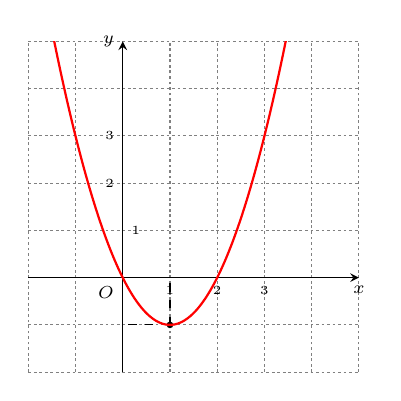
\begin{tikzpicture}[>=stealth,x=1cm,y=1cm,scale=0.6,font=\tiny]
			\def\a{1}
			\def\b{-2}
			\def\c{0}
			\draw[color=gray,dash pattern=on 1pt off 1pt,xstep=1.0cm,ystep=1.0cm] (-2,-2) grid (5,5);
			\draw[->] (-2,0) -- (5,0) node[below] {\scriptsize $x$};
			\draw[->] (0,-2) -- (0,5) node[left] {\scriptsize $y$};
			\draw (0,0)node[below left]{\scriptsize $O$};
			\fill (0,1) node[right]{$1$};
			\fill (0,2) node[left]{$2$};
			\fill (0,3) node[left]{$3$};
			\fill (1,0) node[below]{$1$};
			\fill (2,0) node[below]{$2$};
			\fill (3,0) node[below]{$3$};
			\pgfmathsetmacro\xdinh{-(\b)/2*(\a)}
			\pgfmathsetmacro\ydinh{(4*(\a)*(\c)-(\b)^2)/(4*(\a))}
			\fill[dashed] (\xdinh,\ydinh)circle(2pt) edge (\xdinh,0) edge (0,\ydinh);
			\clip (-2,-2)rectangle(5,5);
			\draw[red,thick,samples=150,smooth,domain=-5:5] plot(\x,{\a*(\x)^2+(\b)*\x+(\c)});
		\end{tikzpicture}	
		&
		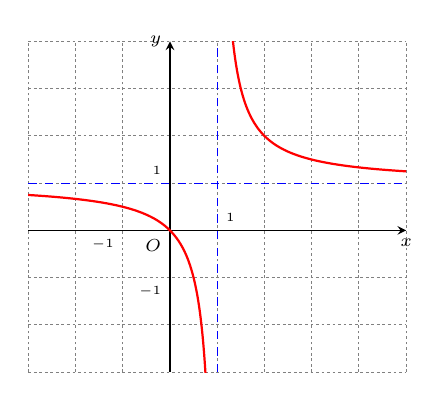
\begin{tikzpicture}[>=stealth,x=1cm,y=1cm,scale=0.6,font=\tiny]
			\def\a{1}
			\def\b{0}
			\def\c{1}
			\def\d{-1}
			\draw[color=gray,dash pattern=on 1pt off 1pt,xstep=1.0cm,ystep=1.0cm] (-3,-3) grid (5,4);
			\draw[->] (-3,0) -- (5,0) node[below] {\scriptsize $x$};
			\draw[->] (0,-3) -- (0,4) node[left] {\scriptsize $y$};
			\draw (0,0)node[below left]{\scriptsize $O$};
			\draw[dashed,blue] (1,-3)--(1,4) (-3,1)--(5,1);
			\fill (-1,0) node[below left]{$-1$};
			\fill (1,0) node[above right]{$1$};
			\fill (0,-1) node[below left]{$-1$};
			\fill (0,1) node[above left]{$1$};
			\clip (-3,-3)rectangle(5,4);
			\pgfmathsetmacro{\can}{-(\d)/(\c)}
			\draw[thick,samples=150,smooth,domain=-5:{\can-.1},red] plot(\x,{(\a*\x+(\b))/(\c*\x+(\d))});
			\draw[thick,samples=150,smooth,domain={\can+.1}:5,red] plot(\x,{(\a*\x+(\b))/(\c*\x+(\d))});
		\end{tikzpicture}
		&
		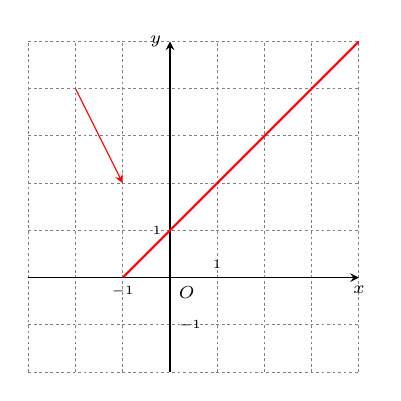
\begin{tikzpicture}[>=stealth,x=1cm,y=1cm,scale=0.6,font=\tiny]
			\def\a{1}
			\def\b{1}
			\draw[color=gray,dash pattern=on 1pt off 1pt,xstep=1.0cm,ystep=1.0cm] (-3,-2) grid (4,5);
			\draw[->] (-3,0) -- (4,0) node[below] {\scriptsize $x$};
			\draw[->] (0,-2) -- (0,5) node[left] {\scriptsize $y$};
			\fill (-1,0) node[below]{$-1$};
			\fill (1,0) node[above]{$1$};
			\fill (0,-1) node[right]{$-1$};
			\fill (0,1) node[left]{$1$};
			\draw (0,0)node[below right]{\scriptsize $O$};
			\draw[red,->] (-2,4)--(-1,2);
			\clip (-1,0)rectangle(4,5);
			\draw[thick,samples=150,smooth,domain=-5:5,red] plot(\x,{\a*\x+(\b)});
		\end{tikzpicture}
		\\
		a) Đồ thị hàm số \break $ f(x)=x^{2}-2x $
		&
		b) Đồ thị hàm số \break $ g(x)=\dfrac{x}{x-1} $
		&
		c) Đồ thị hàm số \break$ h(x)=\heva{&-2x \text{ nếu } x<-1\\&x+1 \text{ nếu }x\geq 1} $
		\\
		&\hspace*{1.5cm}Hình 15& \\
	\end{longtable}
	\loigiai{
		Hàm số liên tục trên tập xác định là $ f(x)=x^{2}-2x $. Vì đồ thị hàm số ở hình \textit{Hình 15a} là một đường liền nét trên mặt phẳng tọa độ. 
	}
\end{bt}

% từ: cau-hoi/lop11/1D3_Gioi_han_Ham_so_lien_tuc/1D3-3-5_Bai_toan_phuong_trinh_co_nghiem.tex
\begin{ex}%[1D3H3-5]%[ma:0dcf0d0c]
	 Phương trình nào dưới đây có nghiệm trong khoảng $\left(0; 1\right)$
	 \choice
		 {$2x^2-3x+4=0$}
		{$\left(x-1\right)^5-x^7-2=0$} 
		 {$3x^4-4x^2+5=0$}
		 {\True $3x^{2017}-8x+4=0$}
	\loigiai{ 
		Xét hàm  số $f(x)=3x^{2017}-8x+4$.
		Hàm số liên tục  trên đoạn $\left[0; 1\right]$ và $f(0)\cdot f(1)=4\cdot (-1)=-4<0$.
		Vậy phương trình $3x^{2017}-8x+4=0$  có nghiệm trong khoảng $\left(0; 1\right)$.
	} 
\end{ex}

% từ: cau-hoi/lop11/1D3_Gioi_han_Ham_so_lien_tuc/1D3-3-5_Bai_toan_phuong_trinh_co_nghiem.tex
\begin{ex}%[1D3H3-5]%[ma:c417dc69]
 Xét tính đúng sai của các khẳng định  sau?
 \choiceTF 
  {\True Phương trình $x^4+mx^2-2mx-2=0$ luôn có nghiệm với mọi giá trị của tham số $m$} 
  {Phương trình $3x^6-3x^3+5x-2=0$ \textbf{không} có nghiệm  thuộc khoảng $(-2;2)$}
  {\True Phương trình $x^3-3x+1=0$ có ba nghiệm  phân biệt}
  {\True Phương  trình $m(x-1)^2(x-2)+2x-3=0$ luôn có nghiệm với mọi giá trị của tham số $m$}
 \loigiai{ 
  \begin{itemchoice}
   \itemch Hàm số $f(x)=x^4+mx^2-2mx-2$ liên tục trên đoạn $[0;2]$, có  $f(0)\cdot f(2) = -2\cdot 14 = -28<0$ nên phương trình $f(x)=0$ có ít nhất một nghiệm thuộc khoảng $(0;2)$ với mọi $m$ hay phương trình $x^4+mx^2-2mx-2=0$ luôn có nghiệm với mọi giá trị của tham số $m$.
   \itemch Hàm số $g(x)=3x^6-3x^3+5x-2$ liên tục  trên đoạn $[0;1]$, có $g(0)\cdot g(1) = -2\cdot 3 =-6<0$ nên phương trình $g(x)=0$ có ít nhất một nghiệm thuộc khoảng $(0;1)$ hay phương trình $g(x)=0$ có nghiệm thuộc khoảng $(-2;2)$.
   \itemch Hàm số $h(x)=x^3-3x+1$ liên tục trên các đoạn $[-2;0]$, $[0;1]$, $[1;2]$ và có  $h(-2)=-1$, $h(0)=1$, $h(1)=-1$, $h(2)=3$.\\
   Do $h(-2)\cdot h(0)<0$, $h(0)\cdot h(1)<0$, $h(1)\cdot h(2)<0$ nên phương trình $h(x)=0$ có ba nghiệm $x_1\in (-2;0)$, $x_2\in (0;1)$, $x_3\in (1;2)$ là  ba nghiệm phân biệt.\\
   Mặt khác phương trình $h(x)=0$ là phương trình bậc  ba nên có không quá ba nghiệm.\\
   Vậy phương trình $h(x)=0$ có ba nghiệm  phân biệt.
   \itemch Hàm số $p(x)=m(x-1)^2(x-2)+2x-3$ liên tục  trên đoạn $[1;2]$, có $p(1)\cdot p(2) = (-1)\cdot 1 = -1<0$ nên phương trình $p(x)=0$ luôn có nghiệm thuộc khoảng $(1;2)$ với mọi $m$ hay phương trình $m(x-1)^2(x-2)+2x-3=0$ luôn có nghiệm với mọi giá trị của tham số $m$.
  \end{itemchoice}
 } 
\end{ex}

% từ: cau-hoi/lop11/1D3_Gioi_han_Ham_so_lien_tuc/1D3-3-6_Toan_thuc_te_ap_dung_ham_so_lien_tuc.tex
\begin{bt}%[1D3H3-6]%[ma:91657403]
% nguon: Archive/2024/TOAN_11_XE/TOAN_11_XE/data4/11C5/KNTT-5.3.tex #718
%[Phạm Hoàng Điệp - Dự Án tex  11 mới]
	\immini{Hình bên cạnh biểu thị độ cao $ h $ (m) của một quả bóng được đá lên thời gian $ t $ (s), trong đó $ h(t)= -2t^{2}+8t $.
		\begin{enumerate}
			\item Chứng tỏ hàm số $ h(t) $ liên tục trên tập xác định.
			\item Dựa và đồ thì hãy xác định $ \displaystyle\lim\limits_{t\to 2}\left(-2t^{2}+8t\right) $.
		\end{enumerate}
	}
	{		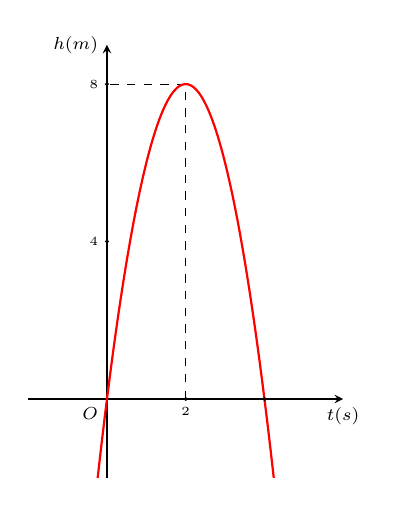
\begin{tikzpicture}[>=stealth,x=1cm,y=1cm,scale=0.5,font=\tiny]
			\def\a{-2}
			\def\b{8}
			\def\c{0}
			\draw[->] (-2,0) -- (6,0) node[below] {\scriptsize $t(s)$};
			\draw[->] (0,-2) -- (0,9) node[left] {\scriptsize $h(m)$};
			\draw (0,0)node[below left]{\scriptsize $O$};
			\fill (0,4) node[left]{$4$};
			\fill (0,8) node[left]{$8$};
			\fill (2,0) node[below]{$2$};
			\draw[dashed] (2,0)--(2,8)--(0,8);
			\pgfmathsetmacro\xdinh{-(\b)/2*(\a)}
			\pgfmathsetmacro\ydinh{(4*(\a)*(\c)-(\b)^2)/(4*(\a))}
			\clip (-2,-2)rectangle(6,9);
			\draw[red,thick,samples=150,smooth,domain=-5:5] plot(\x,{\a*(\x)^2+(\b)*\x+(\c)});
			\foreach \x in {2,4} \draw (\x,0) circle (1pt);
			\foreach \y in {4,8} \draw (0,\y) circle (1pt);
	\end{tikzpicture}}
	\loigiai{
		\begin{enumerate}
			\item Hàm số trên là hàm đa thức nên liên tục trên $ \mathbb{R} $.
			\item Dựa vào đồ thị ta có $  \displaystyle\lim\limits_{t\to 2}\left(-2t^{2}+8t\right) =8 $.
		\end{enumerate}
	}
\end{bt}

% từ: cau-hoi/lop11/1D6_Ham_so_mu_va_ham_so_logarit/1D6-2-3_Rut_gon_chung_minh_bieu_thuc_logarit.tex
\begin{ex}%[1D6H2-3]%[ma:95110287]
	 Cho $a < 0, b > 0$. Mệnh đề nào sau đây \textbf{sai}?
	 \choice
		{$\sqrt[4]{a^4 b^8}=a b^2$} 
		{$\sqrt[4]{a^4 b^8}=\left|a b^2\right|$} 
		{$\sqrt[4]{a^4 b^8}=|a|b^2$} 
		{\True $\sqrt[4]{a^4  b^8}=-a b^2$}
	\loigiai{ 
		Ta có $\sqrt[4]{a^4 b^8}=\left|a b^2\right| = |a|\cdot \left|b^2\right| =  -ab^2$.
	 }
\end{ex}

% từ: cau-hoi/lop11/1D6_Ham_so_mu_va_ham_so_logarit/1D6-3-3_Su_bien_thien_va_do_thi_cua_ham_so_mu_logarit.tex
\begin{ex}%[1D6N3-3]%[ma:21c63876]
	\immini{ 
	Đường cong  trong hình vẽ bên là đồ thị của hàm số nào dưới đây?
	\choice 
		 {$y=-\mathrm{e}^x$}
		{$y=\left|\ln x\right|$} 
		 {\True $y=\ln x$}
		 {$y=\mathrm{e}^x$}
		} 
		{\begin{tikzpicture}[scale=1,line join=round,line cap=round,>=stealth,font=\footnotesize]
		\draw[->] (-0.5,0)--(0,0) node[below  left]{$O$}--(4,0) node[below]{$x$};
		\draw[->] (0,-1.5)  --(0,2) node[right]{$y$};
		\begin{scope}
			\clip (-0.5,-1.5) rectangle (4,2); 
			 \draw[domain=0.25:4,samples=100]plot (\x,{ln(\x)});
		\end{scope}
		\draw[dashed] (2.7,0) node[below]{$\mathrm{e}$}  -- (2.7,1) -- (0,1) node[left]{$1$};
		\draw  (1,0) node[below]{$1$};
		\draw[fill] (0,0)  circle (1pt)
			(0,1) circle  (1pt)
			(1,0)  circle (1pt)
			 (2.7,0) circle (1pt)
			(2.7,1) circle (1pt); 
	\end{tikzpicture}
		} 
	 \loigiai{
		Đồ thị hàm số đi qua điểm $(\mathrm{e};1)$ và nằm cả trên và dưới trục hoành nên chỉ có hàm số $y=\ln  x$ thoả mãn.
	 }
\end{ex}

% từ: cau-hoi/lop11/1D6_Ham_so_mu_va_ham_so_logarit/1D6-3-3_Su_bien_thien_va_do_thi_cua_ham_so_mu_logarit.tex
\begin{ex}%[1D6H3-3]%[ma:781491bc]
	\immini{Đồ thị hình bên là đồ thị  của hàm số nào sau đây?
	 \choice
		{$y=2^x$} 
		 {$y=\left(\dfrac{1}{2}\right)^x$}
		{$y=\left(\dfrac{1}{3}\right)^x$} 
		 {\True $y=3^x$}}
		{\begin{tikzpicture}[>=stealth,scale=0.7,line join=round,line cap=round]
		\def\xp{2} \def\yt{4} \def\yd{-1.2} 
		\draw[->]  (-2,0)--(\xp,0) node [below]{$x$};
		\draw[->]  (0,\yd)--(0,\yt) node [left]{$y$};
		\node at  (0,0) [below left]{$O$};
		\foreach  \p/\r in {1/180}
		 \fill (0,\p) circle (1pt) node[shift={(\r:3mm)}]{$\p$};
		 \draw[dashed] (1,0) node [below]{$1$}--(1,3)--(0,3) node [left]{$3$};
		\begin{scope}
			\clip (-2,-1.2) rectangle  (2.5,4);
			\draw[samples=200,domain=-3:3,smooth,variable=\x] plot (\x,{(3)^(\x)}); 
		\end{scope}
	\end{tikzpicture}
		 }
	 \loigiai{
		 Đồ thị hàm số đi qua điểm $(1;3)$ nên hàm số thỏa mãn là $y=3^x$.
	 }
\end{ex}

% từ: cau-hoi/lop11/1D6_Ham_so_mu_va_ham_so_logarit/1D6-3-3_Su_bien_thien_va_do_thi_cua_ham_so_mu_logarit.tex
\begin{ex}%[1D6V3-3]%[ma:72e32243]
	\immini{Cho ba số thực  dương $a$, $b$, $c$ khác $1$. Đồ thị các hàm số $y=a^x$, $y=b^x$, $y=c^x$ được cho trong hình vẽ bên. Mệnh đề nào dưới đây đúng?
	 \choice
		{$b<c<a$} 
		 {$c<a<b$}
		 {$a<b<c$}
		{\True $a<c<b$}}{\begin{tikzpicture}[scale=1,font=\footnotesize,line join=round,line cap=round,>=stealth,x=0.6cm,y=0.6cm,declare function={f (\x)=2^(\x); g (\x)=3^(\x); h (\x)=0.5^(\x);}]
		\def \xmin{-3.0}; 
		\def \xmax{3.5}; 
		\def \ymin{-1.0}; 
		\def  \ymax{5.5};
		 \draw[->] (\xmin,0.) -- (\xmax,0.) node[anchor=north] {$x$};
		\draw[->] (0.,\ymin) -- (0.,\ymax) node[anchor=west]  {$y$};
		\clip  (\xmin+0.1,\ymin+0.1) rectangle (\xmax-0.1,\ymax-0.1);
		\draw[smooth,samples=100,domain=\xmin:\xmax]  plot (\x,{f (\x)}) plot (\x,{g (\x)}) plot (\x,{h (\x)});
		\draw (-2,\ymax) node[right,rotate=-70]{$y=a^x$} 
			 (1.2,\ymax) node[left,rotate=80]{$y=b^x$}
			(2.3,\ymax-2) node[right,rotate=70]{$y=c^x$}; 
		\foreach  \x/\y/\l/\g in {0/0/O/225,0/1/1/180}{\fill[black] (\x,\y) circle (1pt)+(\g:0.5) node{$\l$};}
	\end{tikzpicture}
		 }
	\loigiai{ 
	\immini{Đường thẳng $x=1$ cắt đồ thị các  hàm số $y=a^x,y=b^x,y=c^x$ tại các điểm có tung độ lần lượt là $y=a$, $y=b$, $y=c$ như hình vẽ bên.\\
		Từ đồ thị kết luận $a<c<b$.}{\begin{tikzpicture}[scale=1,font=\footnotesize,line join=round,line cap=round,>=stealth,x=0.6cm,y=0.6cm,declare function={f (\x)=2^(\x); g (\x)=3^(\x); h (\x)=0.5^(\x);}]
		\def \xmin{-3.0}; 
		\def \xmax{3.5}; 
		\def  \ymin{-1.0};
		 \def \ymax{5.5};
		 \draw[->] (\xmin,0.) -- (\xmax,0.) node[anchor=north] {$x$};
		\draw[->] (0.,\ymin) -- (0.,\ymax) node[anchor=west]  {$y$};
		\clip (\xmin+0.1,\ymin+0.1) rectangle  (\xmax-0.1,\ymax-0.1);
		\draw[smooth,samples=100,domain=\xmin:\xmax]  plot (\x,{f (\x)}) plot (\x,{g (\x)}) plot (\x,{h (\x)});
		 \draw (-2,\ymax) node[right,rotate=-70]{$y=a^x$}
			 (1.2,\ymax) node[left,rotate=80]{$y=b^x$}
			(2.3,\ymax-2)  node[right,rotate=70]{$y=c^x$};
		\draw[dashed](1,0) node[below]{$1$}|-(0,3)  node[left]{$b$}
			 (1,2)--(0,2) node[left]{$c$}
			(1,0.5)--(0,0.5)  node[left]{$a$};
		\foreach \x/\y/\l/\g in {0/0/O/225,0/1/1/180,1/0.5//0,1/2//0,1/3//0,1/0//0,0/0.5//0,0/2//0,0/3//0}{\fill[black] (\x,\y) circle  (1pt)+(\g:0.5) node{$\l$};}
	\end{tikzpicture}
		} 
	 }
\end{ex}

% từ: cau-hoi/lop11/1D6_Ham_so_mu_va_ham_so_logarit/1D6-3-3_Su_bien_thien_va_do_thi_cua_ham_so_mu_logarit.tex
\begin{ex}%[1D6V3-3]%[ma:f8d704c6]
	\immini[thm]{ 
	Cho hai hàm số $y=a^x$, $y=b^x$ với $a$, $b$ là các số dương khác $1$  có đồ thị là $(C_1)$, $(C_2)$ như hình vẽ. Vẽ đường thẳng $y=c$, $(c>1)$ cắt trục tung và $(C_1)$, $(C_2)$ lần lượt tại $M$, $N$, $P$. Biết rằng $S_{OMN}=3S_{ONP}$. Tìm mối liên hệ giữa $a$ và $b$.
	 }{
	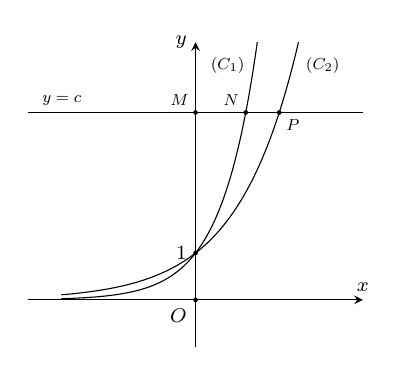
\begin{tikzpicture}[scale=0.85,font=\footnotesize,line join=round,line cap=round,>=stealth,y=0.7cm]
			 \draw[->] (-2.5,0)--(2.5,0) node[above]{$x$};
			 \draw[->] (0,-1)--(0,5.5) node[left]{$y$};
			\begin{scope}
				\clip (-2.5,-1)  rectangle (2.5,5.5);
				\draw (-2.5,4)--(2.5,4); 
				 \draw[samples=200,domain=-2:2.5,smooth,variable=\x] plot (\x,{6.35^(\x)});
				\draw[samples=200,domain=-2:2.5,smooth,variable=\x]  plot (\x,{3.03^(\x)});
			\end{scope}
			\foreach \x/\y  in{0/0,0/1,0/4,0.75/4,1.25/4}{
				 \fill (\x,\y) circle (1pt);
			} 
			\path 
				node at (0,0)[below left]{$O$} 
				node at (0,1)[left]{$1$} 
				node  at (0.75,4)[above left,scale=0.8]{$N$}
				node at  (1.25,4)[below right,scale=0.8]{$P$}
				node at  (0,4)[above left,scale=0.8]{$M$}
				node at (0.48,5)[scale=0.8]{$(C_{1})$} 
				node at (1.9,5)[scale=0.8]{$(C_{2})$} 
				node at (-2,4)[scale=0.8,above]{$y=c$}; 
		\end{tikzpicture}
	 }
	\loigiai{ 
		Đường thẳng $y=c$ cắt $(C_1)$,  $(C_2)$ lần lượt tại hai điểm $N$ và $P$ có hoành độ $x_{N}=\log_{a} c$ và $x_{P}=\log_{b}c$.\\
		 Vì $S_{OMN}=3S_{ONP}$ nên $S_{OMN}=\dfrac{3}{4}S_{OMP}$
		\begin{eqnarray*}
			\Rightarrow \dfrac{1}{2}OM \cdot MN  = \dfrac{3}{4} \cdot \dfrac{1}{2} OM \cdot MP & \Leftrightarrow & MN =\dfrac{3}{4} MP \\
			 & \Leftrightarrow & x_{N}=\dfrac{3}{4}x_{P}\\
			& \Leftrightarrow & \log_{a}c = \dfrac{3}{4} \log_{b}c \\ &  \Leftrightarrow & \dfrac{\log_{b}c}{\log_{b}a}= \dfrac{3}{4} \log_{b}c
			\\ & \Leftrightarrow  & \log_{b}a = \dfrac{4}{3} \Leftrightarrow a^3=b^4.
		\end{eqnarray*}
	 }
\end{ex}

% từ: cau-hoi/lop11/1D6_Ham_so_mu_va_ham_so_logarit/1D6-3-3_Su_bien_thien_va_do_thi_cua_ham_so_mu_logarit.tex
\begin{bt}%[1D6H3-3]%[ma:2e04fb41]
% nguon: Archive/SP-4Phan-Dot3/Data/CD_1_OTGK2_De03.tex #4260
%
Xét tính biến thiên và vẽ đồ thị hàm số $y=\dfrac{1}{3^x}$.
\loigiai{
Ta có $y=\dfrac{1}{3^x}=\left(\dfrac{1}{3}\right)^x$.\\
Tập xác định $\mathscr{D}=\mathbb{R}$.\\
Do cơ số là $\dfrac{1}{3}<1$ nên hàm số nghịch biến trên $\mathbb{R}$.
Với $x=-2 \Rightarrow y=9$ nên đồ thị hàm số đi qua điểm $A(-2;9)$.\\
Bảng biến thiên
\begin{center}
	
\begin{tikzpicture}
		\tkzTabInit[nocadre=false,lgt=1.2,espcl=2.5,deltacl=0.6] 
		{$x$/.6, $f(x)$/2} % cột đầu tiên
		{$-\infty$,$+\infty$} % hàng 1 cột 2
		\tkzTabVar{+/ $+\infty$ , -/ $0$} % hàng 3 cột 2
	\end{tikzpicture}	
\end{center}
Ta có bảng giá trị
			\begin{center}
				\begin{table}[htp]
					\renewcommand{\arraystretch}{2}
					\centering
					\begin{tabular}{|>{$}c<{$}|*{5}{>{$}c<{$}|}}
						\hline
						x & -2 & -1 & 0 & 1 & 2\\
						\hline
						y & 9 & 3 & 1 & \dfrac{1}{3} & \dfrac{1}{9}\\
						\hline
					\end{tabular}
				\end{table}
			\end{center}	
Đồ thị của hàm số $y=\left(\dfrac{1}{3}\right)^x$\\
			\begin{center}
				\begin{tikzpicture}[scale=0.5,>=stealth]
					\def \xmin{-3.1}
					\def \xmax{2.5}
					\def \ymin{-0.7}
					\def \ymax{9.5}
					\draw[->] (\xmin,0) -- (\xmax,0);
					\draw[->,color=black] (0,\ymin) -- (0,\ymax);
					\draw[color=black](\xmax-0.3,.2)node[right] {$x$};
					\draw[color=black] (.1,\ymax) node[right] {\normalsize $y$};
					\begin{scope}
						\clip(\xmin ,\ymin) rectangle (\xmax-.3,\ymax-.3);
						%Vẽ đồ thị
						\draw[color=black,smooth,samples=100,domain=-4.08:4.06] 
						plot(\x,{3^(-\x)});
					\end{scope}
					%vẽ râu ria
					\draw[dashed] (-2,0)node[below]{\tiny $-2$}|-(0,9)node[right]{\tiny $9$} (-1,0)node[below]{\tiny $-1$}|-(0,3)node[right]{\tiny $3$} (1,0)node[below]{\tiny $1$}|-(0,1/3)  (2,0)node[below]{\tiny $2$}|-(0,1/9) (0,0)node[below right]{\tiny $O$}
					(0,1)node[right]{\tiny $1$};
				\end{tikzpicture} 
			\end{center}
			
	} 
\end{bt}

% từ: cau-hoi/lop11/1D6_Ham_so_mu_va_ham_so_logarit/1D6-3-4_So_sanh_cac_luy_thua_va_logarit.tex
\begin{ex}%[1D6N3-4]%[ma:08adbbe6]
 Cho $a^{\frac{3}{4}}>a^{\frac{4}{5}},\log_b\dfrac{1}{2}<\log_b\dfrac{2}{3}$. Khi đó 
  \choiceTF
  {$a>1, 0<b<1$} 
  {$a>1, b>1$} 
   {$0<a<1, 0<b<1$}
  {\True $0<a<1, b>1$} 
 \loigiai{Ta có $\dfrac{3}{4}<\dfrac{4}{5}$, kết hợp  với $a^{\frac{3}{4}}>a^{\frac{4}{5}}$, suy ra $0<a<1$.\\
  Ta có $\dfrac{1}{2}<\dfrac{2}{3}$, kết hợp $\log_b\dfrac{1}{2}<\log_b\dfrac{2}{3}$  suy ra $b>1$.\\
 Vậy  $0<a<1, b>1$.}
\end{ex}

% từ: cau-hoi/lop11/1D6_Ham_so_mu_va_ham_so_logarit/1D6-4-4_Phuong_trinh_mu_logarit_dua_ve_cung_co_so.tex
\begin{ex}%[1D6H4-4]%[ma:5008eed0]
	Có bao nhiêu  số nguyên $x$ thỏa mãn $\log_3(4x-1)-2\log_{\tfrac{1}{9}}(x+2)-2\le0$.
	\loigiai{Điều kiện: $\heva{&4x-1>0\\&x+2>0}\Leftrightarrow\heva{&x>\dfrac{1}{4}\\&x>-2}\Leftrightarrow  x>\dfrac{1}{4}$.\\
		Biến  đổi bất phương trình ta được
		\begin{eqnarray*}
			&&\log_3(4x-1)-2\log_{\tfrac{1}{9}}(x+2)-2\le0\\ 
			&\Leftrightarrow&\log_3(4x-1)+\log_3(x+2)\le2\\ 
			&\Leftrightarrow&\log_3((4x-1)(x+2))\le2\\ 
			 &\Leftrightarrow&4x^2+7x-2\le9\\
			 &\Leftrightarrow&4x^2+7x-11\le0\Leftrightarrow-\dfrac{11}{4}\le x\le1.
		\end{eqnarray*}
	 So điều kiện, nghiệm bất phương trình là $\dfrac{1}{4}<x\le1$, vậy có đúng một giá trị nguyên của $x$ thỏa mãn bài toán.}
\end{ex}

% từ: cau-hoi/lop11/1D6_Ham_so_mu_va_ham_so_logarit/1D6-4-4_Phuong_trinh_mu_logarit_dua_ve_cung_co_so.tex
\begin{bt}%[1D6N4-4]%[ma:8b80327c]
% nguon: Archive/2024/TOAN_11_XE/TOAN_11_XE/data4/11C6/KNTT-6.4.tex #1029
%[TeX hóa SGK 11 - CTST - Đoàn Mạnh Hùng]
	Giải các phương trình sau
	\begin{listEX}[3]
		\item $5^{2 x-1}=25$.
		\item $3^{x+1}=9^{2 x+1}$.
		\item $10^{1-2 x}=100000$.
	\end{listEX}
	\loigiai{
		\begin{listEX}[1]
			\item $5^{2 x-1}=25\Leftrightarrow 5^{2 x-1}=5^2\Leftrightarrow 2x-1=2\Leftrightarrow x=\dfrac{3}{2}$.
			\item $3^{x+1}=9^{2 x+1}\Leftrightarrow 3^{x+1}=3^{4x+2}\Leftrightarrow x+1=4x+2\Leftrightarrow x=-\dfrac{1}{3}$.
			\item $10^{1-2x}=100000\Leftrightarrow 10^{1-2x}=10^5\Leftrightarrow 1-2x=5\Leftrightarrow x=-2$.
		\end{listEX}
	}
\end{bt}

% từ: cau-hoi/lop11/1D6_Ham_so_mu_va_ham_so_logarit/1D6-4-5_Bat_phuong_trinh_mu_logarit_dua_ve_cung_co_so.tex
\begin{bt}%[1D6H4-5]%[ma:8efdaf67]
	\begin{listEX}[2]
		\item $\log  _{3}^{2}x-4\log _{3}x+3>0$.
		\item $\log  _{0,5}^{2}x+2\log _{\sqrt{2}}x<5$.
	\end{listEX}
	 \loigiai{
		\begin{enumerate}
			\item $\log _{3}^{2}x-4\log  _{3}x+3>0$.\\
			Điều kiện:  $x>0$.\\
			Ta  có
			$$\log _{3}^{2} x-4 \log _{3}x+3>0 \xrightarrow{\log _{3}x=t} t^{2}-4 t+3>0 \Leftrightarrow\hoac{&t<1\\&t>3} 
			\Leftrightarrow \hoac{&\log  _3x< 1\\&\log _{3}x>3}\Leftrightarrow \hoac{&x<3\\&x>27.}$$
			Kết hợp với điều kiện, ta được  tập nghiệm $S=(0;3)\cup(27;+\infty)$.
			\item  $\log _{0,5}^{2}x+2\log _{\sqrt{2}}x<5$.\\
			 Điều kiện $x>0$.\\
			$$ 
			\begin{aligned}
				& \log _{\tfrac{1}{2}}^{2} x+2 \log _{\sqrt{2}} x<5  \Leftrightarrow \log _{2}^{2} x+4 \log _{2} x-5<0 \\
				& \xrightarrow{t=\log _{2} x} t^{2}+4 t-5<0 \Leftrightarrow-5<t<1 \Leftrightarrow-5<\log _{2} x<1 \Leftrightarrow  2^{-5}<x<2.
			\end{aligned}
			$$ 
			Kết hợp với điều kiện, ta được tập nghiệm  $S=\left(2^{-5};2\right)$.
		\end{enumerate}
	 }
\end{bt}

% từ: cau-hoi/lop11/1D6_Ham_so_mu_va_ham_so_logarit/1D6-4-5_Bat_phuong_trinh_mu_logarit_dua_ve_cung_co_so.tex
\begin{ex}%[1D6H4-5]%[ma:b86e838f]
	\begin{listEX}[2]
		\item $\log _{3}^{2}x-4\log  _{3}x+3>0$.
		\item  $\log _{0,5}^{2}x+2\log _{\sqrt{2}}x<5$.
	\end{listEX}
	 \loigiai{
		\begin{enumerate}
			\item $\log _{3}^{2}x-4\log  _{3}x+3>0$.\\
			 Điều kiện: $x>0$.\\
			Ta  có
			$$\log  _{3}^{2} x-4 \log _{3}x+3>0 \xrightarrow{\log _{3}x=t} t^{2}-4 t+3>0 \Leftrightarrow\hoac{&t<1\\&t>3}
			\Leftrightarrow \hoac{&\log _3x< 1\\&\log _{3}x>3}\Leftrightarrow \hoac{&x<3\\&x>27.}$$ 
			 Kết hợp với điều kiện, ta được tập nghiệm $S=(0;3)\cup(27;+\infty)$.
			 \item $\log _{0,5}^{2}x+2\log _{\sqrt{2}}x<5$.\\
			 Điều kiện $x>0$.\\
			$$ 
			\begin{aligned}
				& \log _{\tfrac{1}{2}}^{2} x+2 \log _{\sqrt{2}} x<5 \Leftrightarrow \log _{2}^{2}  x+4 \log _{2} x-5<0 \\
				& \xrightarrow{t=\log _{2} x} t^{2}+4 t-5<0 \Leftrightarrow-5<t<1 \Leftrightarrow-5<\log _{2} x<1 \Leftrightarrow  2^{-5}<x<2.
			\end{aligned}
			 $$
			Kết hợp  với điều kiện, ta được tập nghiệm $S=\left(2^{-5};2\right)$.
		\end{enumerate}
	 }
\end{ex}

% từ: cau-hoi/lop11/1D6_Ham_so_mu_va_ham_so_logarit/1D6-4-5_Bat_phuong_trinh_mu_logarit_dua_ve_cung_co_so.tex
\begin{bt}%[1D6V4-5]%[ma:dd7d6687]
	Giải  các bất phương trình sau
	\begin{listEX}[2]
		\item $3^{2x+1} -4\cdot  3^x+1>0$;
		\item $9^x - 5 \cdot 3^x +6  <0$.
	\end{listEX}
	\loigiai{ 
		\begin{listEX}
			\item Ta có  $3^{2x+1}-4\cdot 3^x+1>0 \Leftrightarrow 3\cdot 3^{2x}-4\cdot 3^x+1>0$.\\
			Đặt $t=3^x$, $t>0$, bất phương trình  trên trở thành $$3t^2-4t+1>0 \Leftrightarrow \hoac{&t>1\\&t<\dfrac{1}{3}.}$$
			Với $t>1$, ta có $3^x>1 \Leftrightarrow x  >0$.\\
			Với $t<-1$, ta có  $3^x<\dfrac{1}{3} \Leftrightarrow x<-1$.\\
			Vậy  tập nghiệm của bất phương trình là $S=(-\infty;-1)\cup (1;+\infty)$.
			\item Ta có $9^x-5  \cdot 3^x+6<0 \Leftrightarrow \left(3^2\right)^x-5\cdot 3^x+6<0 \Leftrightarrow \left(3^x\right)^2 -5 \cdot 3^x+6<0. \quad (*)$\\
			Đặt $t=3^x$,  $t>0$, bất phương trình $(*)$ trở thành $$t^2-5t+6<0 \Leftrightarrow 2<t<3.$$
			Với $2<t<3$ ta có $2<3^x<3 \Leftrightarrow \log_3  2 <x<1$.\\
			Vậy  tập nghiệm của bất phương trình là $S=\left(\log_3 2;1\right)$.
		\end{listEX}
	 }
\end{bt}

% từ: cau-hoi/lop11/1D6_Ham_so_mu_va_ham_so_logarit/1D6-5-1_Phuong_phap_dat_an_phu_cho_PT_mu_logarit.tex
\begin{ex}%[1D6C5-1]%[ma:47e4ae9a]
	 \immini
	{ 
	Cho hàm số $y=f(x)$ có đồ thị như hình bên. Có tất cả bao nhiêu giá trị nguyên dương của tham số $m$  nhỏ hơn $2024$ để phương trình $9^{f(x)}+9m=m\cdot3^{f(x)}+3^{f(x)+2}$ có đúng 3 nghiệm thực phân biệt.
	} 
	{ 
	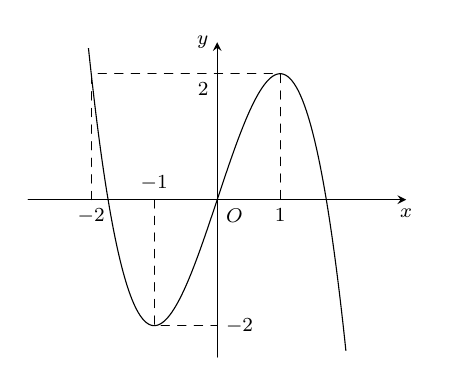
\begin{tikzpicture}[scale=.8,>=stealth,font=\footnotesize,line join=round,line cap=round]
			\def\a{-1} \def\b{0} \def\c{3} \def\d{0} 
			\def\xmin{-3} \def\xmax{3} 
			\def\ymin{-2.5} \def\ymax{2.5} 
			\draw[->]  (\xmin,0)--(\xmax,0) node [below]{$x$};
			\draw[->] (0,\ymin)--(0,\ymax) node [left]{$y$}; 
			\node at (0,0) [below right]{$O$}; 
			\clip (\xmin+0.1,\ymin+0.1) rectangle (\xmax-0.1,\ymax-0.1); 
			\draw[smooth,samples=300] plot (\x,{\a*(\x)^3+\b*(\x)^2+\c*(\x)+\d}); 
			\draw[dashed] (-2,0) node[below]{$-2$}--(-2,2)--(1,2)--(1,0)  node[below]{$1$}
				(-1,0) node[above]{$-1$}--(-1,-2)--(0,-2)  node[right]{$-2$}
				(0,2)  node[below left]{$2$};
		\end{tikzpicture}
	 }
	 \shortans{2014}
	 \loigiai{
		\centerline{ 
		$\begin{aligned}
		 &\ 9^{f(x)}+9m=m\cdot 3^{f(x)}+3^{f(x)+2} \\
		\Leftrightarrow  &\ 3^{2f(x)}-3^{f(x)+2}=m\left(3^{f(x)}-9\right)\\
		\Leftrightarrow &\ 3^{f(x)}\left( 3^{f(x)}-9 \right)=m\left( 3^{f(x)}-9 \right)\\ 
		\Leftrightarrow &\ \left[\begin{aligned}
		& 3^{f(x)}=9 \\ 
		 & 3^{f(x)}=m \\
	\end{aligned} \right.\\
	\Leftrightarrow &\ \left[\begin{aligned}
	& f(x)=2  &(1) \\
	& f(x)=\log_3m &(2) \\ 
	\end{aligned} \right.\\
	(1) \Leftrightarrow f(x)=2 \Leftrightarrow &\ \left[\begin{aligned}
	& x=-2 \\ 
	& x=1.  \\
	\end{aligned} \right.
	\end{aligned}$
	}\\ 
	Để phương trình có  đúng ba nghiệm thực phân biệt
	$\Leftrightarrow (2)$ có đúng 1 nghiệm thực khác $-2$ và  $1$\\
	$$\Leftrightarrow \left[\begin{aligned}
	& 2<\log_3m  \\
	 & \log_3m<-2 \\
	\end{aligned} \right. \Leftrightarrow
	\left[\begin{aligned}
	& m>9  \\
	 & m<\dfrac{1}{9}. \\
	\end{aligned} \right.$$
	Với  $m$ nguyên dương và nhỏ hơn $2024$ nên ta lấy
	$\left\{ \begin{aligned}
	& m\in \mathbb{Z} \\ 
	& 10\le m\le 2023.  \\
	\end{aligned} \right.$\\
	Vậy có $2014$ giá trị của tham  số $m$ thỏa mãn.
	} 
\end{ex}

% từ: cau-hoi/lop11/1D7_Dao_ham/1D7-1-1_Tinh_dao_ham_bang_dinh_nghia.tex
\begin{ex}%[1D7N1-1]%[ma:27a86d1a]
 Cho hàm số $y=f(x)$ có đạo hàm tại $x_0$ là $f'(x_0)$.  Hãy chỉ ra tính đúng, sai của các khẳng định sau?
 \choiceTF 
  {\True  $f'(x_0)=\lim \limits_{x\to x_0} \dfrac{f(x)-f(x_0)}{x-x_0}$}
  {\True  $f'(x_0)=\lim \limits_{\Delta x\to 0} \dfrac{f(x_0+\Delta x)-f(x_0)}{\Delta x}$}
   {\True $f'(x_0)=\lim \limits_{h\to 0} \dfrac{f(x_0+h)-f(x_0)}{h}$}
  {$f'(x_0)=\lim \limits_{x\to x_0} \dfrac{f(x+x_0)-f(x_0)}{x-x_0}$} 
  \loigiai{
  Hàm số $y=f(x)$ có đạo hàm tại $x_0$ là $f'(x_0) \Rightarrow f'(x_0)=\lim \limits_{x\to x_0}  \dfrac{f(x)-f(x_0)}{x-x_0}$.\\
   Đặt $h=\Delta x=x-x_0\Rightarrow f'(x_0)=\lim \limits_{\Delta x\to 0} \dfrac{f(x_0+\Delta x)-f(x_0)}{\Delta x}=\lim \limits_{h\to 0} \dfrac{f(x_0+h)-f(x_0)}{h}$.\\
 Vậy  chỉ có khẳng định $f'(x_0)=\lim \limits_{x\to x_0} \dfrac{f(x+x_0)-f(x_0)}{x-x_0}$ sai, các khẳng định còn lại đúng.}
\end{ex}

% từ: cau-hoi/lop11/1D7_Dao_ham/1D7-2-1_Tinh_dao_ham.tex
\begin{ex}%[1D7H2-1]%[ma:6642d6bb]
	Cho hàm  số $f(x)=\sin^22x$. Tính $f'(x)$.
	\choice 
		 {$f'(x)=2\sin2x$}
		 {$f'(x)=2\cos^22x$}
		{\True  $f'(x)=2\sin4x$}
		 {$f'(x)=-2\sin4x$}
	 \loigiai{Ta có $f'(x)=2\cdot\sin2x\cdot (\sin2x)'=2\cdot\sin2x\cdot 2\cdot\cos2x=2\cdot\sin4x$.
	} 
\end{ex}

% từ: cau-hoi/lop11/1D7_Dao_ham/1D7-2-1_Tinh_dao_ham.tex
\begin{ex}%[1D7Y2-1]%[ma:b1d41e6b]
	Hàm số $y = \sin \left( \dfrac{\pi  }{2} - 2x \right)$ có đạo hàm bằng
	\choice 
		{$y'  = 2\sin 2x$}
		{\True $y' = - 2\sin 2x$} 
		{$y'  = \cos \left( \dfrac{\pi }{2} - 2x \right)$}
		{$y' = 2\cos \left( \dfrac{\pi }{2}  - 2x \right)$}
	 \loigiai{
		Ta có $y=\cos 2x$ nên $y'=-2\sin  2x$.
	 }
\end{ex}

% từ: cau-hoi/lop11/1D7_Dao_ham/1D7-2-1_Tinh_dao_ham.tex
\begin{ex}%[1D7N2-1]%[ma:e2eb2689]
 Cho bốn hàm số $f(x)=\sin x$, $g(x)=\cos  x$, $h(x)=\tan x$ và $k(x)=\cot x$. Xét tính đúng sai của các mệnh đề sau
 \choiceTF 
  {\True $f'(x)=\cos  x, \forall x\in\mathbb{R}$}
  {$g'(x)=\sin  x, \forall x\in\mathbb{R}$}
  {\True $h'(x)=\dfrac{1}{\cos^2x}, \forall x\neq  \dfrac{\pi}{2}+k\pi\left(k\in\mathbb{Z}\right)$}
   {$k'(x)=\dfrac{1}{\sin^2x}, \forall x\neq k\pi, \left(k\in\mathbb{Z}\right)$}
 \loigiai{ 
  \begin{itemchoice}
   \itemch Đúng vì $f'(x)=\cos x, \forall  x\in\mathbb{R}$.
    \itemch Sai vì $g'(x)=-\sin x, \forall x\in\mathbb{R}$.
   \itemch  Đúng vì $h'(x)=\dfrac{1}{\cos^2x}, \forall x\neq\dfrac{\pi}{2}+k\pi, \left(k\in\mathbb{Z}\right)$.
   \itemch Sai vì $k'(x)=-\dfrac{1}{\sin^2x}, \forall x\neq  k\pi, \left(k\in\mathbb{Z}\right)$.
  \end{itemchoice}
 } 
\end{ex}

% từ: cau-hoi/lop11/1D7_Dao_ham/1D7-3-3_Toan_thuc_te_va_Y_nghia_Vat_ly_cua_dao_ham_ca.tex
\begin{ex}%[1D7V3-3]%[ma:ba647522]
	Một vật chuyển động có vận tốc (m/s) được cho bởi hàm số bậc hai có đồ thị như hình vẽ sau 
	\begin{center}
		\begin{tikzpicture}[scale=1,font=\footnotesize,line join=round,line cap=round,>=stealth,declare function = {f (\x) =2*(\x)^2-4*(\x)-1;}]
				 \def \xmin{-1.5};
				 \def \xmax{2.8};
				 \def \ymin{-3.8};
				 \def \ymax{1.5};
				\draw[->] (\xmin,0.) --  (\xmax,0.) node[anchor=north] {$x$};
				\draw[->] (0.,\ymin)  -- (0.,\ymax) node[anchor=west] {$y$};
				\clip (\xmin+0.1,\ymin+0.1) rectangle  (\xmax-0.1,\ymax-0.1);
				\draw[smooth,samples=100,domain=\xmin:\xmax]  plot (\x,{f (\x)});
				\draw[dashed] (1,0) node[above]{$1$} |- (0,-3)  node[left]{$-3$};
				\foreach \x/\y/\l/\g  in {0/0/O/45,1/0//0,0/-3//0,0/-1/-1/180,1/-3//0}{\fill[black] (\x,\y) circle (1pt)+(\g:0.3) node{$\l$};}
			\end{tikzpicture}
	\end{center}
	Biết gia tốc của vật tại thời điểm vận tốc bị triệt tiêu là $a\sqrt{b}$ m/s$^2$, trong đó $a,b\in\mathbb{N}^*$ và  $b\leq 10$. Tính $2a+3b$.
	\shortans{22} 
	\loigiai{ 
		Gọi hàm số bậc  hai cần xác định là $y=ax^2+bx+c$, ($a\neq 0$).\\
		Tọa độ  đỉnh $I(1;-3)\Rightarrow\dfrac{-b}{2a}=1\Leftrightarrow2a+b=0$.\\
		Điểm $I(1;-3)$ thuộc đồ thị hàm số  nên $a+b+c=-3$.\\
		 Đồ thị cắt $Oy$ tại $(0;-1)\Rightarrow c=-1$.\\
		Do đó  ta có hệ phương trình $\heva{&2a+b=0\\&a+b+c=-3\\&c=-1}\Leftrightarrow\heva{&a=2\\&b=-4\\&c=-1.}$\\
		Như thế,  vận tốc của vật là $v(x)=2x^2-4x-1$.\\
		Ta  có
		$v(x)=0\Leftrightarrow 2x^2-4x-1=0\Leftrightarrow\hoac{&x=\dfrac{2+\sqrt{6}}{2}&&\\  &x=\dfrac{2-\sqrt{6}}{2}&& \text{(loại).}}$\\
		Gia tốc của vật  là $a(x)=4x-4$.\\
		Gia tốc của vật  tại thời điểm vận tốc triệt tiêu là $a\left(\dfrac{2+\sqrt{6}}{2}\right)=4\cdot\dfrac{2+\sqrt{6}}{2}-4=2\sqrt{6}$.\\
		Vậy $a=2$, $b=6$  và $2a+3b=4+18=22$.
	} 
\end{ex}

% từ: cau-hoi/lop11/1D9_Xac_suat/1D9-2-4_Quy_tac_cong_cho_hai_bien_co_bat_ki.tex
\begin{bt}%[1D9H2-4]%[ma:811f573e]
% nguon: Archive/SP_DA_SauLuoi/1-TL-TN-THPT-Nhu-Van-Lan-Hai-Phong-HKII-NH23-24.tex #2422
]%[Dự án đề kiểm tra Toán 11 HKII NH23-24- Phạm Quốc Toàn]%[THPT Nhữ Văn Lan- Hải Phòng]
Ba người cùng bắn vào một bia. Xác suất bắn trúng đích của người thứ nhất, thứ hai, thứ ba lần lượt là $0{,}7$; $0{,}6$; $0{,}8$. Xác suất để có đúng hai người bắn trúng đích (làm tròn đến hàng phần trăm)?
\shortans[1]{$0{,}45$}
\loigiai
{
Gọi $A_i$ là biến cố \lq\lq Người thứ $i$ bắn trúng đích\rq\rq\, với $i \in \left\{1;2;3\right\}$.\\
Gọi $B$ là biến cố \lq\lq Có đúng hai người bắn trúng bia\rq\rq.\\
Khi đó $B=A_1A_2\overline{A_3}\cup \overline{A_1}A_2A_3\cup A_1\overline{A_2}A_3$.\\
Ta có 
\begin{eqnarray*}
\mathrm{P} \left(B \right) &=& \mathrm{P} \left(A_1A_2\overline{A_3} \right)+\mathrm{P} \left(\overline{A_1}A_2A_3 \right)+\mathrm{P} \left(A_1\overline{A_2}A_3 \right) \\ 
& = & \mathrm{P} \left(A_1 \right) \cdot \mathrm{P} \left(A_2 \right)\cdot \mathrm{P} \left(\overline{A_3} \right)+\mathrm{P} \left(\overline{A_1} \right)\cdot \mathrm{P} \left(A_2 \right)\cdot \mathrm{P} \left(A_3 \right)+\mathrm{P} \left(A_1 \right)\cdot \mathrm{P} \left(\overline{A_2} \right) \cdot \mathrm{P} \left(A_3 \right) \\ 
& = & 0,7 \cdot 0,6 \cdot 0,2+0,3 \cdot 0,6 \cdot 0,8+0,7 \cdot 0,4 \cdot 0,8 \approx 0,45.
\end{eqnarray*}
}
\end{bt}

% từ: cau-hoi/lop11/1D9_Xac_suat/1D9-2-5_Tinh_xac_suat_bien_co_hop_bang_so_do_hinh_cay.tex
\begin{bt}%[1D9H2-5]%[ma:700a3070]
% nguon: Archive/2024/Update-SP-BG10-11-3/SP-3/BG11-3/data_1C5/DS11-C5-B2-Dang6-SoDoHinhCay-TranTony.tex #1491
%[Bài giảng 11, Trần Tony]
	Gieo ngẫu nhiên một đồng xu và một con xúc xắc. Sử dụng sơ đồ hình cây mô tả số phần tử của không gian mẫu.
	\loigiai{
		\immini{
			Dựa vào sơ đồ hình cây ta thấy không gian mẫu có $12$ phần tử như sau\\
			$\Omega =\{S1; S2;S3;S4;S5;S6;N1;N2;N3;N4;N5;N6\}$.
		}{
			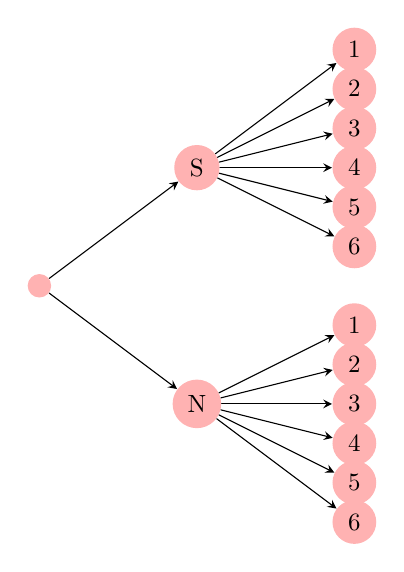
\begin{tikzpicture}[>=stealth,scale=1, line join=round, line cap=round]
				\node[circle, fill=red!30] (a) at (0,0)  {};
				\node[circle, fill=red!30] (b) at (2,1.5)  {\text{S}};
				\node[circle, fill=red!30] (c) at (2,-1.5)  {\text{N}};
				\node[circle, fill=red!30] (d1) at (4,3)  {$1$};
				\node[circle, fill=red!30] (d2) at (4,2.5)  {$2$};
				\node[circle, fill=red!30] (d3) at (4,2)  {$3$};
				\node[circle, fill=red!30] (d4) at (4,1.5)  {$4$};
				\node[circle, fill=red!30] (d5) at (4,1)  {$5$};
				\node[circle, fill=red!30] (d6) at (4,0.5)  {$6$};
				
				\node[circle, fill=red!30] (e1) at (4,-3)  {$6$};
				\node[circle, fill=red!30] (e2) at (4,-2.5)  {$5$};
				\node[circle, fill=red!30] (e3) at (4,-2)  {$4$};
				\node[circle, fill=red!30] (e4) at (4,-1.5)  {$3$};
				\node[circle, fill=red!30] (e5) at (4,-1)  {$2$};
				\node[circle, fill=red!30] (e6) at (4,-0.5)  {$1$};
				\draw[->](a)--(b);\draw[->](a)--(c);
				\draw[->](b)--(d1);\draw[->](b)--(d2);\draw[->](b)--(d3);\draw[->](b)--(d4);\draw[->](b)--(d5);\draw[->](b)--(d6);
				\draw[->](c)--(e1);\draw[->](c)--(e2);\draw[->](c)--(e3);\draw[->](c)--(e4);\draw[->](c)--(e5);\draw[->](c)--(e6);
			\end{tikzpicture}
		}
	}
\end{bt}

% từ: cau-hoi/lop11/1H4_Duong_thang_mat_phang_Quan_he_song_song/1H4-6-3_Xac_dinh_yeu_to_song_song.tex
\begin{ex}%[1H4V6-3]%[ma:3cfcf993]
 Cho hình chóp $ S.ABCD $ có  đáy $ ABCD $ là hình bình hành tâm $O$. Gọi $ M $ là trung điểm $ SB $.
  \choiceTF
  {\True Giao tuyến của đường  thẳng $ (MCD) $ và mp$ (SAB) $ là đường thẳng qua $M$ và song song $AB$}
  {Ba giao tuyến của ba mặt  phẳng $(MAB)$, $(MCD)$, $(ABCD)$ đồng quy}
  {\True Giao điểm  $ H $ của đường thẳng $ MD $ và $ (SAC) $ thuộc cạnh $SO$}
  {\True Gọi $ G $ là trọng tâm tam giác $ ACD $, $ L $ là giao điểm của đường thẳng $ AG $ và $ BC $; $ T $ là giao điểm của $ SC $ và $ (AGM) $. Khi đó ba  điểm $ L, M, T $ thẳng hàng}
 \loigiai{ 
  \begin{center}
   \begin{tikzpicture}[scale=1,font=\footnotesize,line join=round,line cap=round,>=stealth]
     \def\bc{4} 
     \def\ba{2.5} 
      \def\h{5}
     \def\gocB{40} 
     \coordinate[label=below left:$B$] (B)  at (0,0);
     \coordinate[label=above  left:$A$] (A) at (\gocB:\ba);
     \coordinate[label=below:$C$]  (C) at (\bc,0);
     \coordinate[label=right:$D$] (D) at  ($(C)-(B)+(A)$);
     \coordinate[label=above:$S$] (S) at  ($(A)+(0:.5)+(90:\h)$);
     \coordinate[label=below:$O$] (O) at ($(A)!.5!(C)$); 
     \coordinate[label=left:$M$] (M) at  ($(S)!.5!(B)$);
     \coordinate[label=above right:$H$]  (H) at ($(S)!2/3!(O)$);
      \coordinate[label=above:$G$] (G) at ($(D)!2/3!(O)$);
     \coordinate[label=below left:$T$]  (T) at ($(S)!2/3!(C)$);
     \coordinate[label=right:$L$] (L) at ($(C)-(B)+(C)$); 
     \coordinate[label=right:$N$] (N)  at ($(S)!.5!(A)$);
     \draw  (B)--(C)--(D)--(S)--cycle (S)--(C)
       ($(C)!.5!(D)$)--(L);
      \draw[dashed] (C)--(A)--(D)--(B)
      (O)--(S)--(A)--(B) 
       (A)--($(C)!.5!(D)$)
      (D)--(M)--(N); 
      \draw[red](L)--(M);
     \foreach \diem in {A,B,C,D,S,G,M,H,T,L,O,N} \fill (\diem)  circle (1pt);
    \end{tikzpicture}
  \end{center}
  \begin{itemchoice}
   \itemch Đúng. Ta có $ M \in (MCD) $ và $ M \in SB \subset (SAB) $ nên $M$ là điểm chung thứ nhất  của hai mặt phẳng $ (MCD) $ và $ (SAB) $. \\
   Mặt khác, $ DC \subset (MDC) $, $ AB  \subset (SAB) $ và $ AB \parallel CD $. \\
   Nên giao tuyến cần tìm là đường thẳng $ d  $ đi qua $ M $ và song song với $ AB $ và cắt $ SA $ tại trung điểm $ N $.
   \itemch Sai. Ta có $(MAB)\cap(MCD)=d$,  $(MAB)\cap(ABCD)=AB$,\\$(MCD)\cap(ABCD)=CD$ nên $d\parallel AB\parallel CD$.
   \itemch Đúng. Trong mp$ (SBD)  $ gọi $H$ là giao điểm của $ SO $ và $ DM $. \\
   Khi đó $ H \in SO \subset (SAC)$, $H \in DM $ nên  $ H = DM \cap (SAC) $.\\
   Suy ra Giao điểm $ H $ của đường thẳng $ MD $ và  $ (SAC) $ thuộc cạnh $SO$
   \itemch Đúng. Ta  có $ L = AG \cap BC \Rightarrow L \in (AGM) \cap (SBC)$. \\
   Ta có $ M \in SB \subset (SBC) \Rightarrow M \in (AGM) \cap  (SBC)$. \\
   Ta có $ N =  SG \cap (AGM) \Rightarrow N \in (AGM) \cap (SBC)$. \\
   Từ đó $ L, M, N $ cùng thuộc giao tuyến của hai mặt phẳng $ (AGM) $ và $ (SBC)  $ nên $ L, M, N $ thẳng hàng.
  \end{itemchoice}
 } 
\end{ex}

% từ: cau-hoi/lop11/1H8_Quan_he_vuong_goc_trong_khong_gian/1H8-1-3_Tim_goc_giua_hai_duong_thang.tex
\begin{ex}%[1H8H1-3]%[ma:a52f4749]
 Cho hình chóp $ S.ABCD$, có đáy $ ABCD$ là hình vuông, $ SA\perp\left(ABCD\right)$. Gọi  $ H$, $ K$ lần lượt là hình chiếu vuông góc của $ A$ lên $ SB$, $ SD$.
  \choiceTF
   {\True $ SA\perp CD$}
   {$\Delta SAC$ vuông tại $ C$}
  {$\widehat{SBC}=60^\circ  $}
  {\True  $ AH$ và $ AK$ cùng vuông góc với $ SC$}
 \loigiai{\begin{center}
  \begin{tikzpicture}[font=\footnotesize]
     \def\a{3}
    \def\h{3} 
    \path  (0:0) coordinate (A)
      ++(0:\a) coordinate (D)
     ++(-130:\a/2)  coordinate (C)
      ($(A)+(C)-(D)$) coordinate (B)
     ($(A)+(90:\h)$) coordinate (S) 
     (intersection of A--C  and B--D) coordinate (O)
     ($(S)!0.5!(B)$) coordinate  (H)
     ($(S)!0.5!(D)$) coordinate  (K);
     \draw[dashed,thick] (A)--(H)--(K)--(A)
      (B)--(A)--(D)
     (A)--(S); 
    \draw[thick]  (B)-- (C)--(D)
     (B)--(S) 
     (C)--(S) 
     (D)--(S); 
    \foreach \x/\g  in {H/-180,K/0,A/-80,B/-135,C/-45,D/45,S/90}
    \fill[black] (\x)  circle (1pt)
      ($(\g:3mm)+(\x)$) node {$\x$};
    \draw pic[draw,angle  radius=3mm]{right angle=D--A--S};
   \end{tikzpicture}
 \end{center}\begin{itemchoice} \itemch Đúng. Ta có: $\heva{&
 SA\perp\left(ABCD\right)\\& 
  CD\subset\left(ABCD\right)
  }\Rightarrow SA\perp CD$.
 \itemch Sai. Ta có:  $\heva{&
 SA\perp\left(ABCD\right)\\& 
 AC\subset\left(ABCD\right) 
 }\Rightarrow SA\perp AC$. Vậy $\Delta SAC$ vuông tại  $ A$.
 \itemch Sai. Ta có: $\heva{& 
 BC\perp  SA\left(SA\perp\left(ABCD\right)\right)\\&
 BC\perp AB\left(gt\right)\\& 
 SA,AB\subset\left(SAB\right){\rm{,}}SA\cap  AB=A
 }\\\Rightarrow BC\perp\left(SAB\right)\Rightarrow  BC\perp SB\Rightarrow\widehat{SBC}=90^\circ $.
  \itemch Đúng. Ta có: $\heva{&
 AH\perp SB\left(gt\right)\\& 
  AH\perp BC\left(BC\perp\left(SAB\right)\right)\\&
  SB,BC\subset\left(SBC\right){\rm{;}}SB\cap BC=B
 }\\\Rightarrow AH\perp\left(SBC\right)\Rightarrow AH\perp SC$.\\ 
  $\heva{&
 AK\perp  SD\left(gt\right)\\&
  AK\perp CD\left(CD\perp\left(SAD\right)\right)\\&
 SD,CD\subset\left(SCD\right){\rm{,}}SD\cap CD=D}\\\Rightarrow AK\perp\left(SCD\right)\Rightarrow AK\perp SC$.\\ 
 Vậy $AH$ và $ AK$ cùng vuông góc với $SC$. 
\end{itemchoice}}
\end{ex}

% từ: cau-hoi/lop12/2D1_Ung_dung_dao_ham_de_khao_sat_ham_so/2D1-1-3_Tim_tham_so_de_ham_so_don_dieu.tex
\begin{ex}%[2D1H1-3]%[ma:6d07edea]
	Cho hàm số $y=f(x)$ có bảng biến thiên  như sau.
	Mệnh đề nào  dưới đây là \textbf{sai?}
	\begin{center}
		
\begin{tikzpicture}
			 \tkzTabInit[nocadre = false,lgt = 1,espcl = 3]
				{$x$  /1,$y'$ /1,$y$ /2}{$-\infty$,$0$,$2$,$+\infty$}
			\tkzTabLine{,+,$0$,-,$0$,+,} 
			 \tkzTabVar{-/ $-\infty$,+/ $3$,-/ $0$,+/ $+\infty$}
		\end{tikzpicture}
	\end{center}
	\choice 
		{\True Hàm số \textbf{không}  đạt cực tiểu tại điểm $x=2$}
		{Hàm số  đạt cực đại tại điểm $x=0$}
		{Giá trị cực đại của hàm số là $y=3$} 
		{Giá trị cực  tiểu của hàm số là $y=0$}
	\loigiai{Hàm số đạt cực  tiểu tại điểm $x=2$.}
\end{ex}

% từ: cau-hoi/lop12/2D1_Ung_dung_dao_ham_de_khao_sat_ham_so/2D1-1-4_Ung_dung_tinh_don_dieu_de_chung_minh_bat_dang.tex
\begin{bt}%[2D1N1-4]%[ma:7778b300]
% nguon: Archive/2024/TaiLieuGiangDay/1.HamSo/1. K12 - 4in1 - Hamso/ThubaiGoc/Bai1-Dang4.tex #2644
%%[Mức độ 1]%[Dự án bài giảng new 4in1, Trần Quang Thạnh]
	Dùng phương pháp hàm số, giải phương trình $\log_{3} (x^2+1) =\log_3 (3-x)$.
	\loigiai{
	Điều kiện $x<3$.\\
	Vì hàm số $y=f(t)=\log_{3} t$ đồng biến trên tập xác định của nó nên từ phương trình đã cho, ta có 
	$$f(x^2+1)=f(3-x) \Leftrightarrow x^2+1 =3-x \Leftrightarrow x^2+x-2=0 \Leftrightarrow \hoac{&x=1\\ &x=-2.}$$
	Đối chiếu với điều kiện, ta có tập nghiệm phương trình là $S=\{1;-2\}$.
	}
\end{bt}

% từ: cau-hoi/lop12/2D1_Ung_dung_dao_ham_de_khao_sat_ham_so/2D1-1-4_Ung_dung_tinh_don_dieu_de_chung_minh_bat_dang.tex
\begin{bt}%[2D1H1-4]%[ma:6f3724a5]
% nguon: Archive/2024/TaiLieuGiangDay/1.HamSo/1. K12 - 4in1 - Hamso/ThubaiGoc/Bai1-Dang4.tex #2653
[Mức độ 2]%[Dự án bài giảng new 4in1, Trần Quang Thạnh]
	Giải phương trình $5^x-5^{2x+1}=x+1$.
	\loigiai{
	Phương trình đã cho tương đương với $5^x + x =5^{2x+1}+2x+1$.\\
	Vì hàm số $y=f(t)=5^t+t$ có $y'=5^t\ln5 +1>0$, với mọi $t\in \mathbb{R}$ nên hàm số $y=f(t)$ đồng biến trên $\mathbb{R}$, do đó, từ phương trình đã cho ta được $$f(x)=f(2x+1) \Leftrightarrow x=2x+1 \Leftrightarrow x=-1.$$
	Vậy phương trình đã cho có nghiệm duy nhất $x=-1$.
	}
\end{bt}

% từ: cau-hoi/lop12/2D1_Ung_dung_dao_ham_de_khao_sat_ham_so/2D1-1-4_Ung_dung_tinh_don_dieu_de_chung_minh_bat_dang.tex
\begin{bt}%[2D1H1-4]%[ma:49ecfa36]
% nguon: Archive/2024/TaiLieuGiangDay/1.HamSo/1. K12 - 4in1 - Hamso/ThubaiGoc/Bai1-Dang4.tex #2654
[Mức độ 2]%[Dự án bài giảng new 4in1, Trần Quang Thạnh]
	Giải phương trình $3^x - 3^{x^2-2x} >x^2-3x$.
	\loigiai{
		Phương trình được biến đổi trở thành $3^x + x > 3^{x^2-2x}+x^2-2x$.\\
		Vì hàm số $y=f(t)=3^t$ đồng biến trên $\mathbb{R}$ nên từ phương trình trên ta được
		$$f(x)>f(x^2-2x) \Leftrightarrow x> x^2-2x \Leftrightarrow x^2-3x <0 \Leftrightarrow 0<x<3.$$
		Vậy bất phương trình đã cho có tập nghiệm là $S=(0;3)$.
	}
\end{bt}

% từ: cau-hoi/lop12/2D1_Ung_dung_dao_ham_de_khao_sat_ham_so/2D1-1-5_Toan_thuc_te_ung_dung_su_dong_bien_nghich_bie.tex
\begin{bt}%[2D1V1-5]%[ma:4e47f47a]
% nguon: Archive/SP_SauLuoi_2024-2025/SP_HKI/2-TN-DS-TLN-SGD-VinhLong-HKI-NH24-25.tex #27
%[Dự án đề kiểm tra Khối 12 HK1 NH24-25 - Đợt 5 - Nguyễn Trần Anh Tuấn]%[SGD - Tỉnh Vĩnh Long]
	Một chất điểm chuyển động có phương trình $s(t)$ thì có vận tốc $v(t)=s'(t)$. Biết rằng phương trình chuyển động của chất điểm là $s(t)=\dfrac{1}{3}t^3-3t^2+5t$ trong đó $t$ được tính bằng giây và $s$ được tính bằng mét. Kể từ giây thứ bao nhiêu trở đi thì vận tốc của chất điểm bắt đầu tăng?
	\shortans{3}
	\loigiai{
		Ta có $v(t)=s'(t)=t^2-6t+5$, $t \ge 0$, suy ra $v'(t)=2t-6$.\\
		Lại có $v'(t)=0 \Leftrightarrow t=3$.\\
		Bảng biến thiên
		\begin{center}
			
\begin{tikzpicture}[line join=round,font=\footnotesize,>=stealth, scale=1]
				\tkzTabInit[nocadre=false,lgt=1.2,espcl=2.5,deltacl=0.8]
				{$x$ /1,$v'$ /0.6,$v$ /2}
				{$0$, $3$, $+ \infty$}
				\tkzTabLine{,-,0,+,}
				\tkzTabVar{+/$+ \infty$ ,-/$-4$, +/$+ \infty$}
			\end{tikzpicture}
		\end{center}
		Kể từ giây thứ $3$ trở đi thì vận tốc của chất điểm bắt đầu tăng.
	}
\end{bt}

% từ: cau-hoi/lop12/2D1_Ung_dung_dao_ham_de_khao_sat_ham_so/2D1-1-5_Toan_thuc_te_ung_dung_su_dong_bien_nghich_bie.tex
\begin{bt}%[2D1V1-5]%[ma:eed0a430]
% nguon: Archive/2024/San pham - To Latex Strong - Tex hoa Lop 12 moi - Dot 3 (Chuong 1 + 2 +3 + 4)/Data/Chuong 1/Canh dieu/To 1 - Dot 16 - Chuong 1 - Bai 1 - CD - De 3.tex #3574
%[To 16 - Dot 16 - Chuong 1 - Bai 1 - CD - De 3]%[Đình Nguyên]
	Một chất điểm chuyển động theo phương trình $s(t)=-\dfrac{t^3}{3}+18 t^2-35 t+10$, trong đó $t$ tính bằng giây và $s$ tính bằng mét. Trong 40 giây đầu tiên, chất điểm có vận tốc tức thời giảm trong khoảng thời gian $(a ; b)$. Tính giá trị của biểu thức $P=2 b-3 a$.
	\shortans{26}
	\loigiai{
		Vận tốc tức thời của chất điểm là $v(t)=s'(t)=-t^2+36 t-35$.\\
		Gia tốc tức thời của chất điểm là $a(t)=v'(t)=-2 t+36$.\\
		Vì vận tốc tức thời của chất điểm giảm nên $a(t)<0 \Leftrightarrow-2 t+36<0 \Leftrightarrow t>18$.\\
		Do đó, trong $40$ giây đầu tiên, chất điểm có vận tốc tức thời giảm trong khoảng thời gian $(18 ; 40)$. Suy ra $a=18, b=40$.\\
		Vậy $P=2 b-3 a=26$.
	}
\end{bt}

% từ: cau-hoi/lop12/2D1_Ung_dung_dao_ham_de_khao_sat_ham_so/2D1-2-2_Tim_cuc_tri_dua_vao_BBT_do_thi.tex
\begin{ex}%[2D1N2-2]%[ma:36a07538]
	 \immini{
	Cho hàm số $y=ax^3+bx^2+cx+d \,(a,b,c,d\in \mathbb{R})$ có đồ thị là đường cong trong hình bên. Giá trị cực đại của hàm số đã cho  bằng
	 \choice
		{$0$} 
		 {\True $3$}
		{$1$} 
		 {$-1$}
		 }
		 {
		\begin{tikzpicture}[>=stealth,scale=0.8,font=\footnotesize]
			\draw[->] (-2.5,0)--(3,0) node[below]  {$x$};
			\draw[->] (0,-2)--(0,4) node[left] {$y$}; 
			\draw[domain=-2:2,samples=100]  plot (\x,{-(\x)^3+3*\x+1});
			\draw (0,0) node[below right=-0.1]  {$O$} circle (1.2pt);
			\draw (1,0) node[above right]  {$1$} circle (1.2pt);
			 \draw (-1,0) node[above] {$-1$} circle (1.2pt);
			\draw (0,-1) node[right] {$-1$} circle (1.2pt); 
			\draw  (0,1) node[right] {$1$} circle (1.2pt);
			\draw (0,3) node[left] {$3$}  circle (1.2pt);
			\draw[dashed]  (1,0)--(1,3)--(0,3)
				(-1,0)--(-1,-1)--(0,-1); 
		\end{tikzpicture}
		 }
	\loigiai{ 
	Từ đồ thị hàm số, giá  trị cực đại của hàm số đã cho bằng $3$.}
\end{ex}

% từ: cau-hoi/lop12/2D1_Ung_dung_dao_ham_de_khao_sat_ham_so/2D1-2-2_Tim_cuc_tri_dua_vao_BBT_do_thi.tex
\begin{ex}%[2D1N2-2]%[ma:d4f134b2]
	\immini{Cho hàm số $y=f(x)$ liên tục trên $\mathbb{R}$ và có đồ thị như hình bên. Phát  biểu nào sau đây là đúng?
	\choice 
		{$x_{\text{ CT}}=-1$, $x_{\text{  CĐ}}=1$}
		{$x_{\text{ CT}}=-3$, $x_{\text{ CĐ}}=1$} 
		{$x_{\text{ CT}}=1$, $x_{\text{  CĐ}}=-3$}
		{\True $x_{\text{ CT}}=1$, $x_{\text{ CĐ}}=-1$}} 
		{\resizebox{!}{4cm}{\begin{tikzpicture}[line join=round,line cap=round,>=stealth]
		\draw[->] (-3.1,0)--(3.1,0) node[below left]  {$x$};
		\draw[->] (0,-3.6)--(0,2.5) node[below left] {$y$}; 
		\fill (0,0) circle (1pt) node [below  right] {$O$};
		\draw[dashed,thin](-1,0)  node[below]{$-1$}--(-1,1)--(0,1) node[right]{$1$};
		\draw[dashed,thin](1,0) node[above]{$1$}--(1,-3)--(0,-3)  node[left]{$-3$};
		\begin{scope}
			\clip (-3,-3.5)  rectangle (2.5,2);
			\draw[samples=100,domain=-4:4,smooth,variable=\x] plot  (\x,{((\x)^3)+0*((\x)^2)+-3*(\x)-1});
		\end{scope}
		 \fill (-1,1) circle (1pt)
			(0,-1) circle  (1pt)
			(1,-3) circle  (1pt);
	\end{tikzpicture}
		 }
		 }
	\loigiai{ 
		Dựa  vào đồ thị ta thấy hàm số có $x_{\text{ CT}}=1$, $x_{\text{ CĐ}}=-1$.
	} 
\end{ex}

% từ: cau-hoi/lop12/2D1_Ung_dung_dao_ham_de_khao_sat_ham_so/2D1-2-2_Tim_cuc_tri_dua_vao_BBT_do_thi.tex
\begin{ex}%[2D1H2-2]%[ma:af4b716b]
	 Cho hàm số $y=f(x)$ xác định và liên tục trên $\mathbb{R}$ có bảng biến thiên như hình vẽ. Gía trị nhỏ nhất của hàm số trên khoảng $(-2;+\infty)$ bằng?
	\begin{center}
		
\begin{tikzpicture}
			 \tkzTabInit[nocadre,lgt=1,espcl=2.3]
				{$x$ /0.7,$y'$ /0.7,$y$  /2}
				 {$-\infty$,$-2$,$5$,$+\infty$}
			 \tkzTabLine{,+,0,-,0,+,}
			\tkzTabVar{-/$-\infty$,+/ $1$,-/ $0$  /,+/$+\infty$ /}
		\end{tikzpicture}
	\end{center}
	\choice 
		{\True $0$} 
		 {$1$}
		{$-2$} 
		 {$5$}
	 \loigiai{
		Dựa vào  bảng biến thiên trên khoảng $(-2;+\infty)$
		ta  có giá trị nhỏ nhất là $0$ tại $x=5$.
	 }
\end{ex}

% từ: cau-hoi/lop12/2D1_Ung_dung_dao_ham_de_khao_sat_ham_so/2D1-2-2_Tim_cuc_tri_dua_vao_BBT_do_thi.tex
\begin{bt}%[2D1H2-2]%[ma:eab7f5f7]
% nguon: Archive/2024/TaiLieuGiangDay/1.HamSo/1. K12 - 4in1 - Hamso/ThubaiGoc/Bai2-Dang2.tex #2629
%[BG12, Tran Tony]
	\immini{Cho hàm số $y=f(x)$ liên tục trên đoạn $[0 ; 3]$ thoả mãn\\ $f'\left(\dfrac{1}{3}\right)=f'(1)=f'\left(\dfrac{5}{2}\right)=0$ và có đồ thị là đường cong như hình bên. Tìm cực trị của hàm số đã cho trên khoảng $(0;3)$.
	}{
	\begin{tikzpicture}[scale=0.9, font=\footnotesize, line join=round, line cap=round, >=stealth]
	\tikzset{declare function={xmin=-2;xmax=4;ymin=-3;ymax=2; f(\x)=32/45*(\x)^4-32/9*(\x)^3+224/45*(\x)^2-32/15*(\x);},smooth,samples=450}
	\draw[->] (xmin,0)--(xmax,0) node[shift={(-100:7pt)}]{$ x $};
	\draw[->] (0,ymin)--(0,ymax) node[shift={(190:7pt)}]{$ y $};
	\fill (0,0) node[shift={(135:10pt)}]{$ O $};
	\draw[dashed](1/3,0)node[shift={(90:8pt)}]{$\tfrac{1}{3}$}|-(0,-1/3)node[shift={(-150:9pt)}]{$-\tfrac{1}{3}$}
			(2.5,0)node[shift={(90:7pt)}]{$\tfrac{5}{2}$}|-(0,-2)node[shift={(180:9pt)}]{$-2$}	(1,0)node[shift={(90:7pt)}]{$1$};
	\clip (xmin,ymin) rectangle (xmax,ymax);
	\draw  plot[domain=xmin:xmax] (\x, {f(\x)});
	\end{tikzpicture}}
	\loigiai{
		\begin{itemize}
			\item Hàm số đạt cực tiểu tại $x=\dfrac{1}{3}$, $y_{\text{CT}}=-\dfrac{1}{3}$.
			\item Hàm số đạt cực tiểu tại $x=\dfrac{5}{2}$, $y_{\text{CT}}=-2$.
			\item Hàm số đạt cực đại tại $x=1$, $y_{\text{CĐ}}=0$.
	\end{itemize}
	}
\end{bt}

% từ: cau-hoi/lop12/2D1_Ung_dung_dao_ham_de_khao_sat_ham_so/2D1-2-7_Toan_thuc_te_ung_dung_cuc_tri_cua_ham_so.tex
\begin{bt}%[2D1H2-7]%[ma:b5b08b78]
% nguon: Archive/2024/TaiLieuGiangDay/1.HamSo/1. K12 - 4in1 - Hamso/ThubaiGoc/Bai2-Dang8.tex #2725
%[Bài giảng 12-4in1, Nhật Thiện]
	\immini{Một phần đường ray tàu lượn siêu tốc có dạng đồ thị hàm số bậc ba $y=f(x)=-\dfrac{1}{2\,000}x^3+\dfrac{17}{200}x^2-4x+50$. Trục $Ox$ mô tả quãng đường tàu di chuyển theo chiều ngang (tính bằng centimét), trục $Oy$ mô tả chiều cao của đường ray (tính bằng centimét) tại mỗi vị trí $x$.Tìm tọa độ các cực trị của đường ray trên đoạn $[0;100]$.
}{
	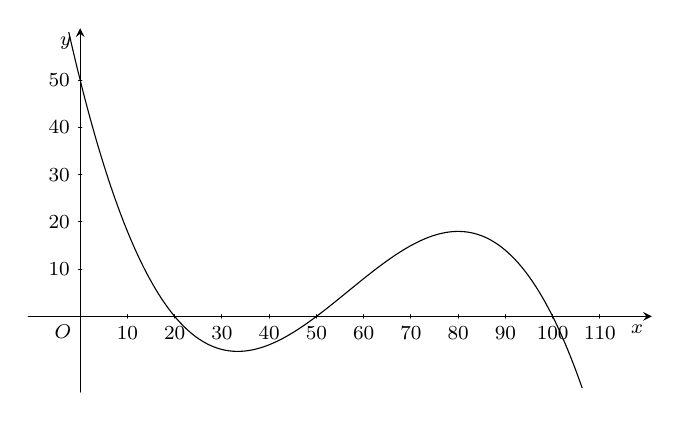
\begin{tikzpicture}[scale=1, font=\footnotesize, line join=round, line cap=round, >=stealth]
		\begin{scope}[scale=.6]
			\draw[->] (-1.1,0)--(12.1,0) node[below left] {$x$};
			\draw[->] (0,-1.6)--(0,6.1) node[below left] {$y$};
			\draw (0,0) node [below left] {$O$};
			\foreach \x/\nx in {1/10,2/20,3/30,4/40,5/50,6/60,7/70,8/80,9/90,10/100,11/110}
			\draw[thin] (\x,1pt)--(\x,-1pt) node [below] {$\nx$};
			\foreach \y/\ny in {1/10,2/20,3/30,4/40,5/50}
			\draw[thin] (1pt,\y)--(-1pt,\y) node [left] {$\ny$};
			\begin{scope}
				\clip (-1,-1.5) rectangle (12,6);
				\draw[samples=200,domain=-1:12,smooth,variable=\x] plot (\x,{(-1/20)*((\x)-2)*((\x)-5)*((\x)-10)});
			\end{scope}
		\end{scope}
	\end{tikzpicture}}
\loigiai{
	Ta có $y'=-\dfrac{3}{2\,000}x^2+\dfrac{17}{100}x-4$.\\
	Xét $y'=0\Leftrightarrow \hoac{&x=\dfrac{100}{3}\\&x=80.}$\\
	Bảng biến thiên
	\begin{center}
		
\begin{tikzpicture}
\tkzTabInit[nocadre=false,lgt=1.2,espcl=2.5,deltacl=0.6]
{$x$ /0.6,$y’$ /0.6,$y$ /2}
{$0$,$\tfrac{100}{3}$,$80$,$100$}
\tkzTabLine{,-,0,+,0,-}
\tkzTabVar{+/$50$,-/$-\tfrac{200}{27}$,+/$18$,-/$0$}
\end{tikzpicture}
	\end{center}
Ta có tọa độ các điểm cực trị của đồ thị hàm số $f(x)$ là $A\left(\dfrac{100}{3};-\dfrac{200}{27}\right)$ và $B(80;18)$.
}
\end{bt}

% từ: cau-hoi/lop12/2D1_Ung_dung_dao_ham_de_khao_sat_ham_so/2D1-3-1_GTLN_GTNN_tren_doan.tex
\begin{ex}%[2D1H3-1]%[ma:f02d1e5d]
	\immini 
	{Bảng biến thiên sau là của đồ thị hàm số  nào sau đây?
	} 
	{
\begin{tikzpicture}
		\tkzTabInit[nocadre,lgt=1.5,espcl=3,deltacl=.5] 
			{$x$/0.7,$f’(x)$/0.7,$f  (x)$/2}
			{$-\infty$,$1$,$+\infty$} 
		 \tkzTabLine{,-,d,-,}
		\tkzTabVar{+/$+\infty$,-D+/  $-\infty$/$+\infty$,-/$-\infty$}
	\end{tikzpicture}
	} 
	 \choice
		 {$y = \dfrac{x+1}{x-1}$}
		{\True $y  = \dfrac{-x^2+2x}{x-1}$}
		{$y = \dfrac{-x^2+x}{x-1}$} 
		{$y =  \dfrac{x+2}{2x-2}$}
	\loigiai{Do $\lim\limits_{x \to 1^+} y = +\infty$  nên đồ thị có tiệm cận đứng là đường thẳng $x=1$.\\
		 Mặt khác $\lim\limits_{x \to +\infty} f(x) = -\infty$ và $\lim\limits_{x \to -\infty} f(x) = +\infty$ nên đồ thị hàm số không có tiệm cận ngang.\\
		Mặt khác  $y = \dfrac{-x^2+x}{x-1} = \dfrac{-1}{x-1}$ nên $\lim\limits_{x \to +\infty} \dfrac{-1}{x-1} = 0$.\\
		Vậy bảng  biến thiên của hàm số $y = \dfrac{-x^2+2x}{x-1}$.
	 }
\end{ex}

% từ: cau-hoi/lop12/2D1_Ung_dung_dao_ham_de_khao_sat_ham_so/2D1-3-1_GTLN_GTNN_tren_doan.tex
\begin{ex}%[2D1H3-1]%[ma:28a3bf6f]
	Giá trị lớn nhất của hàm số $y=x+\cos  ^2x$ trên $\left[0;\dfrac{\pi}{2} \right]$ là
	 \choice
		 {\True $\dfrac{\pi}{2}$}
		 {$\dfrac{\pi}{2}+1$}
		{$1$} 
		{$\dfrac{\pi}{4}+\dfrac{1}{2}$} 
	 \loigiai{
		Ta có: $y=f(x)=x+\cos  ^2x$ trên $\left[0;\dfrac{\pi}{2} \right]$.\\
		$y'=f'(x)=1-2\sin x\cdot \cos x=1-\sin 2x\ge 0$ với mọi $x \in \left[0;\dfrac{\pi}{2} \right]$.\\ 
		Suy ra $\displaystyle \max \limits_{\left[0;\tfrac{\pi}{2} \right]}  f(x) = f \left( \dfrac{\pi }{2}\right)=\dfrac{\pi}{2}$.
	} 
\end{ex}

% từ: cau-hoi/lop12/2D1_Ung_dung_dao_ham_de_khao_sat_ham_so/2D1-3-1_GTLN_GTNN_tren_doan.tex
\begin{bt}%[2D1C3-1]%[ma:4c943e74]
	Cho hàm  đa thức bậc ba $y=f(x)$ có đồ thị như hình vẽ
	\begin{center}
		\begin{tikzpicture}[>=stealth,scale=0.8]
			\draw[->] (-4,0)  --(4,0);
			 \draw[->](0,-4)--(0,4);
			\draw (0,0.7) node[below  left]{$O$};
			 \draw (4,0) node[below]{$x$};
			\draw (0,4) node[left]{$y$}; 
			 \draw (2,0) node[above left]{$2$};
			\draw  (-1,0) node[above left]{$-1$};
			 \draw (0,-1) node[left]{$-1$};
			\draw[dashed] (0,-2) 
				node[left]{$-2$} -- (1,-2) -- 
				(1,0)  node[above]{$1$};
			\clip  (-4,-4) rectangle (4,4);
			 \draw[samples=100] plot[domain=-4:4]
				(\x,{(1/2)*(\x)^3-(3/2)*\x-1}); 
		\end{tikzpicture}
	\end{center}
	Tổng số đường tiệm cận ngang và tiệm cận đứng của đồ thị  $y= \dfrac{(x+1)(x^2-1)}{f(x)}$ là
	\shortans{3} 
	\loigiai{Hàm số  có dạng $f(x)=ax^3+bx^2+cx-1$.
		Đồ thị hàm số đã cho đi qua các điểm $(-1;0)$, $(1;-2)$, $(2;0)$ nên ta  có
		$$\heva{&8a+4b+2c=1\\& -a+b-c=1 \\&a+b+c=-1} \Leftrightarrow  \heva{&a=\dfrac{1}{2}\\&b=0 \\&c=\dfrac{-3}{2}.}$$
		Suy  ra hàm số $f(x)=\dfrac{1}{2}x^3-\dfrac{3}{2}x-1 = \dfrac{1}{2}(x-1)^2(x-2)$.\\
		Khi đó  $y=\dfrac{(x+1)(x^2-1)}{f(x)}=\dfrac{(x+1)(x^2-1)}{\dfrac{1}{2}(x-1)^2(x-2)}=\dfrac{2(x+1)^2}{(x-1)(x-2)}$.\\
		Đồ thị hàm số trên có tiệm cận ngang là đường thẳng $y=2$ và tiệm  cận đứng là các đường thẳng $x=1$, $x=2$.\\
		Vậy đồ thị hàm số  $y = \dfrac{(x+1)(x^2-1)}{f(x)}$ có $3$ đường tiệm cận.
	 }
\end{bt}

% từ: cau-hoi/lop12/2D1_Ung_dung_dao_ham_de_khao_sat_ham_so/2D1-3-2_GTLN_GTNN_tren_khoang.tex
\begin{ex}%[2D1H3-2]%[ma:b8b838ac]
	\immini{Cho hàm số $y=f(x)$ liên tục trên $\mathbb{R}$ và có đồ thị  như hình bên.
	 \choiceTF
		{\True Hàm số nghịch biến trên khoảng  $(0;1)$}
		{Hàm số đồng biến trên khoảng $(-1;2)$} 
		{\True Hàm số có  ba điểm cực trị}
		{Hàm số có giá trị lớn  nhất bằng $2$}
		}{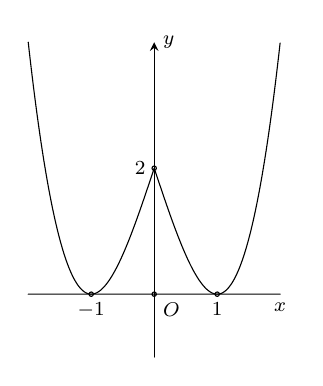
\begin{tikzpicture}[scale=0.8,font=\footnotesize,line join=round,line join=round,line cap = round,>=stealth]
		\draw[->] (-2,0)--(0,0) node[below right]{$O$} circle (1pt)--(2,0)  node[below]{$x$};
		 \draw[->] (0,-1) --(0,4) node[right]{$y$};
		\foreach  \x in {-1,1}{
			\draw  (\x,0) node[below]{$\x$} circle (1pt);}
		\foreach \y in {2}{ 
			\draw (0,\y) node[left]{$\y$} circle (1pt);} 
		 \draw [domain=0:2,samples=100]
			plot  (\x,{(\x)^3-3*(\x)+2});
		 \draw [domain=-2:0,samples=100]
			plot (\x,{-(\x)^3+3*(\x)+2}); 
	\end{tikzpicture}
		 }
	 \loigiai{
		Dựa vào đồ thị hàm số,  ta thấy
		\begin{itemchoice}
			\itemch Hàm số nghịch biến trên khoảng  $(0;1)$ là khẳng định đúng.
			\itemch Hàm số đồng biến trên khoảng $(-1;2)$ là khẳng định sai,  vì trên khoảng $(0;1)$ hàm số nghịch biến.
			\itemch Hàm số  có ba điểm cực trị là khẳng định đúng, hàm số có $3$ điểm cực trị tại $x=-1$, $x=0$, $x=1$.
			\itemch Hàm số có giá trị lớn nhất bằng  $2$ là khẳng định sai, hàm số có giá trị cực đại bằng $2$, không tồn tại giá trị lớn nhất.
		\end{itemchoice}
	} 
\end{ex}

% từ: cau-hoi/lop12/2D1_Ung_dung_dao_ham_de_khao_sat_ham_so/2D1-3-4_Ung_dung_GTNN_GTLN_trong_bai_toan_phuong_trin.tex
\begin{bt}%[2D1N3-4]%[ma:9560f7ae]
% nguon: Archive/2024/TaiLieuGiangDay/1.HamSo/1. K12 - 4in1 - Hamso/ThubaiGoc/Bai3-Dang6.tex #2020
[Mức độ 1]%[BG12-4IN1, Nguyễn Khánh Trọng]
	Cho hàm số $y=f(x)$ có bảng biến thiên như hình vẽ.
	\begin{center}
		
\begin{tikzpicture}
			\tkzTabInit[lgt=1.2,espcl=2]
			{$x$ /.7, $f’(x)$ /.7, $f(x)$ /2}
			{$-\infty$,$-3$,$4$,$+\infty$}
			\tkzTabLine{ ,+,z,-,z,+, }
			\tkzTabVar{-/$-\infty$,+/$2$,-/$-2$,+/$+\infty$}
		\end{tikzpicture}
	\end{center}
	Tìm tất cả giá trị của tham số $m$ để bất phương trình $f(x)\le m$ có nghiệm $x\in(-3;+\infty)$.
	\loigiai{
		Ta có $f(x)\le m$ có nghiệm $x\in(-3;+\infty)$ khi và chỉ khi
		$\min\limits_{(-3;+\infty)}f(x)\le m\Leftrightarrow m\ge -2$.
	}	
\end{bt}

% từ: cau-hoi/lop12/2D1_Ung_dung_dao_ham_de_khao_sat_ham_so/2D1-3-4_Ung_dung_GTNN_GTLN_trong_bai_toan_phuong_trin.tex
\begin{bt}%[2D1V3-4]%[ma:c3918870]
% nguon: Archive/2024/TaiLieuGiangDay/1.HamSo/1. K12 - 4in1 - Hamso/ThubaiGoc/Bai3-Dang6.tex #2034
[Mức độ 3]%[BG12-4IN1, Nguyễn Khánh Trọng]
	Tìm tất cả các giá trị của tham số $m$ để bất phương trình $m\left( x-1 \right)-\sqrt{x-4}\le m+1$ có nghiệm.
	\dapso{$m\in \left( -\infty ;\dfrac{1+\sqrt{3}}{4} \right]$}
	\loigiai{
		Xét bất phương trình $m\left( x-1 \right)-\sqrt{x-4}\le m+1$\quad (1).\\
		Điều kiện xác định của bất phương trình là $x\ge 4$.\\
		Đặt $t=\sqrt{x-4}\Rightarrow t\ge 0$ và $x=t^2+4$, khi đó (1) trở thành
		$m\left(t^2+3 \right)-t\le m+1\Leftrightarrow m\le \dfrac{t+1}{t^2+2}$\quad (2).\\
		Xét hàm số $f(t)=\dfrac{t+1}{t^2+2}$ với $t\ge 0$. Ta có
		$f'(t)=\dfrac{-t^2-2t+2}{(t^2+2)^2}$.\\
		Cho $f'(t)=0\Leftrightarrow -t^2-2t+2=0\Leftrightarrow \hoac{& t=-1+\sqrt{3} \\ & t=-1-\sqrt{3}\,\,(\text{loại}).}$\\
		Bảng biến thiên của hàm số $f(t)$ trên nửa khoảng $[0;+\infty)$.
		\begin{center}
			
\begin{tikzpicture}
				\tkzTabInit[lgt=1.2,espcl=3]
				{$t$ /.7, $f’(t)$ /.7, $f(t)$ /2.5}
				{$0$,$-1+\sqrt{3}$,$+\infty$}
				\tkzTabLine{ ,+,z,- }
				\tkzTabVar{-/$\dfrac{1}{2}$,+/$\dfrac{1+\sqrt{3}}{4}$,-/$0$}
			\end{tikzpicture}
		\end{center}
		Bất phương trình (1) có nghiệm $\Leftrightarrow $ (2) có nghiệm $t\in [0;+\infty)\Leftrightarrow m\le \dfrac{1+\sqrt{3}}{4}$.
	}
\end{bt}

% từ: cau-hoi/lop12/2D1_Ung_dung_dao_ham_de_khao_sat_ham_so/2D1-3-6_Toan_thuc_te_ung_dung_GTLN_GTNN_cua_ham_so.tex
\begin{bt}%[2D1V3-6]%[ma:00caf0ae]
	\immini{Một vật chuyển động với vận tốc $v$ (km/h) phụ thuộc vào thời gian $t$ (h) có đồ thị của hàm số  dạng hàm bậc ba như hình bên. Biết rằng tại thời điểm $t_1=1$ h vật có vận tốc $v_1=4$ km/h và tại thời điểm $t_2=2$ h vật có vận tốc $v_2=1$ km/h. Hỏi vận tốc của vật tại thời điểm $t=3$ h bằng bao nhiêu km/h?}{
	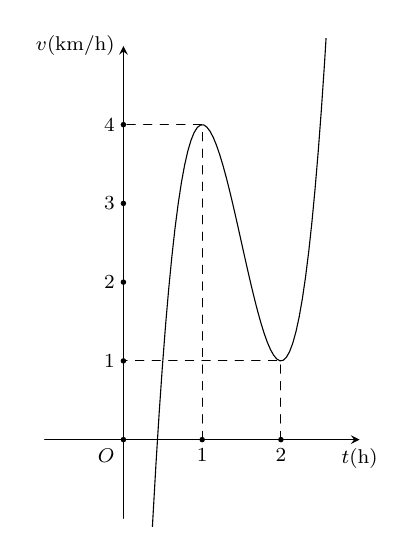
\begin{tikzpicture}[scale=1,font=\footnotesize,line join=round,line cap=round,>=stealth]
		\def\xmin{-1}; \def\ymin{-1}; \def\xmax{3};  \def\ymax{5};
		\coordinate (O) at  (0,0);
		\draw[->]  (\xmin,0)--(\xmax,0) node[below]{$t$(h)};
		 \draw[->] (0,\ymin)--(0,\ymax) node[left]{$v$(km/h)};
		\fill  (O) node[below left]{$O$} circle (1pt);
		 \clip ({\xmin-0.1},{\ymin-0.1}) rectangle ({\xmax+0.1},{\ymax+0.1});
		 \foreach \x in {1,2}{
			\fill (\x,0) node[below]{$\x$}  circle (1pt);
		} 
		\foreach \y in  {1,2,3,4}{
			 \fill (0,\y) node[left]{$\y$} circle (1pt);
		 }
		 \draw[samples=100] plot[domain=-1:3](\x,{6*(\x)^3-27*(\x)^2+36*\x-11});
		\draw[dashed]  (2,0)|-(0,1)
			(1,0)|-(0,4); 
	\end{tikzpicture}
	} 
	 \shortans{16}
	 \loigiai{
		Giả sử hàm số vận tốc có dạng $v(t)=a t^3+b  t^2+c t+d$ (với $a\ne 0$ và $t\ge 0$).\\
		Ta có  $v'(t)=3a t^2+2b t+c$.\\
		Dựa vào đồ thị hàm số, tại các thời điểm $t_1$, $t_2$ đồ thị hàm vận  tốc đi qua các điểm cực trị $A(1;4)$, $B(2;1)$.\\
		Khi đó $\heva{&v(1)=4\\&v'(1)=0\\&v(2)=1\\&v'(2)=0}\Leftrightarrow\heva{&a+b+c+d=4\\&3a+2b+c=0\\&8a+4b+2c+d=1\\&12a+4b+c=0}\Leftrightarrow\heva{&a=6\\&b=-27\\&c=36\\&d=-11.}$\\ 
		Suy  ra $v(t)=6t^3-27t^2+36t-11$ (km/h).\\
		Vậy vận tốc của vật tại thời  điểm $t=3$ h là $v(3)=6\cdot 3^3-27\cdot 3^2+36\cdot 3-11=16$ (km/h).
	 }
\end{bt}

% từ: cau-hoi/lop12/2D1_Ung_dung_dao_ham_de_khao_sat_ham_so/2D1-3-6_Toan_thuc_te_ung_dung_GTLN_GTNN_cua_ham_so.tex
\begin{ex}%[2D1H3-6]%[ma:2a52e637]
% nguon: Archive/SP_SauLuoi_2024-2025/SP_HKI/2-TN-DS-TLN-THPT-DinhTienHoang-NinhBinh-HKI-NH24-25.tex #92
%[Dự án đề kiểm tra Khối 12 HK1 NH24-25 - Đợt 4 - Quang Vinh NT]%[THPT Đinh Tiên Hoàng - Tỉnh Ninh Bình]
	Một vật chuyển động theo quy luật $s(t) = t^3 - 3t^2 + 9t + 36$, với $t$ (giây) là khoảng thời gian tính từ lúc chất điểm bắt đầu chuyển động và $s$ là quãng đường vật đi được trong khoảng thời gian đó, tính bằng mét $(m)$.  
	\choiceTF
	{Quãng đường vật đi được sau $4$ giây kể từ lúc bắt đầu chuyển động là $82$ m}
	{\True Vận tốc của vật tại giây thứ $t$ là $v(t) = 3t^2 - 6t + 9$}
	{Gia tốc của vật tại thời điểm $2$ giây là $4$ $(m/s^2)$}
	{\True Trong khoảng thời gian $10$ (s) đầu tiên, vận tốc của vật nhỏ nhất là $6$ $(m/s)$}
	\loigiai{
		\begin{itemchoice}
			\itemch \textbf{Quãng đường sau $4$ giây:}  
			$$
			s(4) = 4^3 - 3 \cdot 4^2 + 9 \cdot 4 + 36 = 88 \, \text{m}.
			$$
			\itemch \textbf{Vận tốc tại giây thứ $t$:}  
			$$
			v(t) = s'(t) = 3t^2 - 6t + 9.
			$$			
			\itemch \textbf{Gia tốc tại thời điểm $t = 2$:}  
			Gia tốc là đạo hàm bậc hai của $s(t)$, tức là:
			$$
			a(t) = v'(t) =  6t - 6.
			$$
			Tại $t = 2$:
			$$
			a(2) = 6 \cdot 2 - 6 = 12 - 6 = 6 \, \text{m/s}^2.
			$$
			
			\itemch \textbf{Vận tốc nhỏ nhất trong $10$ giây đầu tiên:}  
			Xét hàm vận tốc $v(t) = 3t^2 - 6t + 9$.  
			Đạo hàm của $v(t)$:
			$$
			v'(t) = 6t - 6.
			$$
			Phương trình $v'(t) = 0\Leftrightarrow 			6t - 6 = 0  \Leftrightarrow  t = 1.
			$\\
			Bảng biến thiên 
			\begin{center}
				\begin{tikzpicture}
					\tkzTabInit[lgt=1.5,espcl=2]
					{$t$/1, $v'(t)$/1, $v(t)$/2}
					{$0$, $1$, $10$}
					\tkzTabLine{,+,0,-,}
					\tkzTabVar{+/ $9$, -/ $6$, +/ $249$}
				\end{tikzpicture}
			\end{center}	
			Giá trị nhỏ nhất của $v(t)$ trên $[0; 10]$ là $v(1) = 6 \, \text{m/s}$.
		\end{itemchoice}
	}
\end{ex}

% từ: cau-hoi/lop12/2D1_Ung_dung_dao_ham_de_khao_sat_ham_so/2D1-3-6_Toan_thuc_te_ung_dung_GTLN_GTNN_cua_ham_so.tex
\begin{bt}%[2D1V3-6]%[ma:d59a8e2b]
% nguon: Archive/2024/San pham - To Latex Strong - Tex hoa Lop 12 moi - Dot 2 (Chuong 1 + 2 + 3)/San pham - To Latex Strong - Tex hoa Lop 12 moi - Dot 2 (Chuong 1 + 2 + 3)/Data/Chuong 1/Chan troi sang tao/To 25 - Dot 16 - Chuong 1 - Bai 2 - CTST - De 2.tex #853
%[Tổ 25 - Đợt 16 - Chương 1 - Bài 1 - CTST]%[Nguyen Ngoc Quoc]
Ông $A$ muốn mua một mảnh đất hình chữ nhật có diện tích bằng $100~m^2$ để làm khu vườn. Để chi phí xây dựng bờ rào xung quanh khu vườn là ít tốn kém nhất thì ông $A$ đã mua mảnh đất có kích thước $a(m)\times b(m)$ (với $a$ là chiều dài, $b$ là chiều rộng của khu vườn). Khi đó kết quả của $a+2b$ bằng bao nhiêu?
\shortans{$30$}
\loigiai
{
	Để chi phí xây dựng bờ rào là ít tốn kém nhất thì chu vi mảnh đất phải bé nhất.\\
	Gọi $x$ là chiều dài của mảnh đất hình chữ nhật $(x>0)$. Suy ra chiều rộng là $\dfrac{100}{x}$.\\
	Chu vi của mảnh đất hình chữ nhật là $C(x)=2x+\dfrac{200}{x}$.\\
	Ta có $C'(x)=2-\dfrac{200}{x^2}=\dfrac{2x^2-200}{x^2}$; $C'(x)=0 \Leftrightarrow 2x^2-200=0 \Leftrightarrow x=10~(\text{vì}~x>0)$.
	Bảng biến thiên
	\begin{center}
	\begin{tikzpicture}[thick,scale=1,nodes={scale=1}]
		\tkzTabInit[espcl=4]
		{$x$/0.8,$C'(x)$/.8,$C(x)$/2}
		{$0$,$10$,$+\infty$}
		\tkzTabLine{,-,0,+,}
		\tkzTabVar{+/$+\infty$,-/$40$,+/$+\infty$}
	\end{tikzpicture}
	\end{center}	
	Từ bảng biến thiên ta thấy $\min\limits_{(0;+\infty)} C(x)=C(10)=40$.\\
	Suy ra chu vi mảnh đất hình chữ nhật bé nhất khi chiều dài bằng $10~m$, chiều rộng bằng $10~m$. Vậy $a+2b=30$.
	
}
\end{bt}

% từ: cau-hoi/lop12/2D1_Ung_dung_dao_ham_de_khao_sat_ham_so/2D1-4-1_Bai_toan_xac_dinh_cac_duong_tiem_can_cua_ham.tex
\begin{ex}%[2D1N4-1]%[ma:454844fe]
	\immini{Cho hàm số $f(x)$ có đồ thị như hình bên. Biết rằng một trong bốn đường thẳng sau đây là đường tiệm cận  xiên của đồ thị hàm số, đường đó là đường nào?
	\choice 
		 {$y=2x$}
		{$y=\dfrac{-x}{2}$} 
		{\True  $y=-2x$}
		{$y=\dfrac{x}{2}$} 
		}{\resizebox{!}{5cm}{\begin{tikzpicture}
		 \draw[->] (-3.1,0)--(3.1,0) node[below left] {$x$};
		\draw[->] (0,-3.1)--(0,4.1) node[below  left] {$y$};
		\draw (0,0) node [below left] {$O$}; 
		\foreach \x  in {-2,-1,1,2}
		\draw (\x,1pt)--(\x,-1pt) node  [below] {$\x$};
		\foreach \y  in {-2,-1,1,2}
		\draw (1pt,\y)--(-1pt,\y)  node [left] {$\y$};
		\begin{scope}
			\clip (-3,-3) rectangle (3,4); 
			\draw[samples=100,domain=-3:-0.01,smooth,variable=\x] plot  (\x,{(-2*((\x)^2)+0*(\x)+1)/((\x)+0)});
			 \draw[samples=100,domain=0.01:3,smooth,variable=\x] plot (\x,{(-2*((\x)^2)+0*(\x)+1)/((\x)+0)});
			 \draw (-3.1,6.2)--(3.1,-6.2);
		\end{scope}
	\end{tikzpicture}
		 }}
	\loigiai{ 
		Gọi tiệm cận xiên của đồ thị có dạng  $d \colon y=ax+b$ ($a\ne 0$).\\
		Mà $\heva{&O(0;0) \in  d\\& A(-1;2)\in d} \Rightarrow \heva{&0=b\\&2=-a+b} \Rightarrow \heva{&a=-2\\&b=0}$.\\
	Nên tiệm cận xiên của đồ thị hàm  số là $d\colon y=-2x$.}
\end{ex}

% từ: cau-hoi/lop12/2D1_Ung_dung_dao_ham_de_khao_sat_ham_so/2D1-4-1_Bai_toan_xac_dinh_cac_duong_tiem_can_cua_ham.tex
\begin{ex}%[2D1H4-1]%[ma:b5c045b7]
	 \immini{
	Cho hàm số $y=\dfrac{ax^2+bx+c}{x},(ac  \ne 0)$ có đồ thị như hình bên. Đường tiệm cận xiên của đồ thị hàm số đã cho là đường thẳng
	\choice 
		{Đường thẳng $y=x$} 
		 {\True Đường thẳng $y=-x$}
		{Đường  thẳng $x=0$}
		{Đường thẳng  $y=2x$}
		}{\resizebox{!}{5cm}{\begin{tikzpicture}[scale=0.4,>=stealth,line join=round,line cap=round]
		\draw[->] (-6,0)--(6,0)  node[below]{$x$};
		\draw[->] (0,-7.5)--(0,8) node[left]{$y$}; 
		\draw[samples=100,domain=-6:-0.6] plot  (\x,{-(\x)-4/(\x)});
		 \draw[samples=100,domain=0.6:6] plot (\x,{-(\x)-4/(\x)});
		\draw[samples=100,domain=-6:6] plot  (\x,{(-\x)});
		\draw (0,0) node[below left]{$O$}; 
		\draw[dashed] 
			(0,-4) node[left]{$-4$} 
			 (2,0) node[above left]{$2$}
			(0,4) node[right]{$4$} 
			 (-2,0) node[above left]{$-2$}
			 (-2,0)--(-2,4)--(0,4)
			(2,0)--(2,-4)--(0,-4); 
		\fill (0,0) circle (1pt) 
			(-2,4) circle  (1pt)
			(2,-4) circle (1pt); 
	\end{tikzpicture}
		 }
		 }
	\loigiai{ 
		Dựa vào đồ thị ta thấy hàm số có đường tiệm cận xiên đi qua $O(0;0)$ và là đường đi xuống từ trái sang phải nên $y=-x$ là tiệm  cận xiên của đồ thị hàm số.
	} 
\end{ex}

% từ: cau-hoi/lop12/2D1_Ung_dung_dao_ham_de_khao_sat_ham_so/2D1-4-1_Bai_toan_xac_dinh_cac_duong_tiem_can_cua_ham.tex
\begin{bt}%[2D1H4-1]%[ma:d42c3bf7]
% nguon: Archive/2024/TaiLieuGiangDay/1.HamSo/1. K12 - 4in1 - Hamso/ThubaiGoc/Bai4-Dang3.tex #2455
%CD%[Dự án TL12New-4in1-NCT]
	Đồ thị hàm số ở \texttt{Hình 18a, Hình 18b} đều có đường tiệm cận ngang là đường thẳng màu đỏ. Hỏi đó là đồ thị của hàm số nào trong các hàm số sau?
	
	\begin{tikzpicture}[scale=.7, font=\footnotesize, line join=round, line cap=round, >=stealth]
		\draw[->] (-4,0)--(0,0) node[above right]{$O$}--(5,0) node[below]{$x$};
		\draw[->] (0,-2) --(0,3) node[right]{$y$};
		\draw [domain=-4:5, samples=100] %
		plot (\x, {(2*(\x)^2-2)/((\x)^2+2)});
		\foreach \x/\g in {-1/-100,1/-90} 
		\draw[fill] (\x,0) circle(.5pt)node [shift={(\g:.3)}] {$\x$};
		\foreach \y/\g in {-1/-140,2/135} 
		\draw[fill] (0,\y) circle(.5pt)node [shift={(\g:.3)}] {$\y$};
		%\draw[blue] (1,-4)--(1,5);
		\draw[red!80] (-4,2)--(5,2);
		\draw (2,-2) node{Hình 18a};
	\end{tikzpicture}\hspace{2cm}
	\begin{tikzpicture}[scale=.7, font=\footnotesize, line join=round, line cap=round, >=stealth]
		\draw[->] (-4,0)--(0,0) node[above left]{$O$}--(5,0) node[below]{$x$};
		\draw[->] (0,-2) --(0,2) node[right]{$y$};
		\draw [domain=-4:5, samples=100] %
		plot (\x, {(2*(\x)^2+2*(\x)-1)/(2*(\x)^2+1)});
		\foreach \x/\g in {-2/-90,1/-90} 
		\draw[fill] (\x,0) circle(.5pt)node [shift={(\g:.3)}] {$\x$};
		\foreach \y/\g in {-1/-10,1/135} 
		\draw[fill] (0,\y) circle(.5pt)node [shift={(\g:.3)}] {$\y$};
		%\draw[blue] (1,-4)--(1,5);
		\draw[red!80] (-4,1)--(5,1);
		\draw (2,-2) node{Hình 18b};
	\end{tikzpicture}
	\begin{enumerate}[a)]
		\item$y=\dfrac{x^2+2x-1}{x^2+1}$;
		\item $y=\dfrac{2x^2+x+1}{x-1}$;
		\item $y=\dfrac{2x^2-2}{x^2+2}$.
	\end{enumerate}
	\loigiai{
		\begin{enumerate}[a)]
			\item Ở hình 18a ta thấy đồ thị cắt trục hoành tại $\pm 1$, cắt trục tung tại $-1$ và nhận đường thẳng $y=2$ là tiệm cận ngang và không có tiệm cận đứng. \\
			Vậy trong $3$ hàm số chỉ có hàm $y=\dfrac{2x^2-2}{x^2+1}$ thoả mãn.
			\item Ở hình 18b ta thấy đồ thị có tiệm cận ngang $y=1$ và không có tiệm cận đứng.\\
			Vậy trong $3$ hàm số trên chỉ có hàm số $y=\dfrac{x^2+2x-1}{x^2+1}$ thoả mãn.
		\end{enumerate}
	}
\end{bt}

% từ: cau-hoi/lop12/2D1_Ung_dung_dao_ham_de_khao_sat_ham_so/2D1-4-3_Bai_toan_lien_quan_den_do_thi_ham_so_va_cac_d.tex
\begin{bt}%[2D1C4-3]%[ma:fcc83f8d]
% nguon: Archive/2024/San pham - To Latex Strong - Tex hoa Lop 12 moi - Dot 3 (Chuong 1 + 2 +3 + 4)/Data/Chuong 1/Canh dieu/To 3 - Dot 16 - Chuong 1 - Bai 3 - CD - De 2.tex #3581
%[Tổ 3 - Đợt 16 - Chương 1 - Bài 3 - Cánh Diều - Đề 2]%[Đình Nguyên]
	Cho hàm số $y=f(x)=a x^3+b x^2+c x+d\quad (a \neq 0)$ có đồ thị như hình vẽ bên dưới\\
	\begin{center}
		
		\begin{tikzpicture}[line join=round, line cap=round,>=stealth,thick]
			\tikzset{every node/.style={scale=0.9}}
			\draw[->] (-3.1,0)--(3.1,0) node[above left] {$x$};
			\draw[->] (0,-3.1)--(0,5.1) node[below left] {$y$};
			\draw (0,0) node [below left] {$O$};
			\foreach \x/\nx in {-3/-3,-2/-2,-1/-1,1/1,2/2,3/3}
			\draw[thin] (\x,1pt)--(\x,-1pt) node [below] {$\nx$};
			\foreach \y/\ny in {-3/-3,-2/-2,-1/-1,1/1,2/2,3/3}
			\draw[thin] (1pt,\y)--(-1pt,\y) node [left] {$\ny$};
			\draw[dashed] (-1,0)--(-1,4)--(0,4);
			\begin{scope}
				\clip (-3,-3) rectangle (4,4);
				\draw[samples=200,domain=-3:3,smooth,variable=\x] plot (\x,{1*((\x)^3)+0*((\x)^2)+-3*(\x)+2});
			\end{scope}
		\end{tikzpicture}
		
	\end{center}
	Tìm số đường tiệm cận đứng của đồ thị hàm số $g(x)=\dfrac{\sqrt{x}}{f\left(x^2-1\right)-4}$.
	\loigiai{
		Điều kiện $x \geq 0$. Từ đồ thị, ta có $a > 0$.\\
		Ta có $f(x)-4=0\Leftrightarrow f(x)=4\Leftrightarrow\hoac{&x=-1\\
			&x=\alpha \quad (\alpha > 1)
			&}$ trong đó $x=-1$ là nghiệm kép.\\
		Suy ra $f(x)-4=a(x+1)^2(x-\alpha)$.\\
		Do đó $f\left(x^2-1\right)-4=a x^4\left(x^2-1-\alpha\right)$. \\
		Suy ra $ g(x)=\dfrac{\sqrt{x}}{f\left(x^2-1\right)-4}=\dfrac{\sqrt{x}}{a x^4\left(x^2-1-\alpha\right)}=\dfrac{1}{a x^3 \sqrt{x}(x-\sqrt{1+\alpha})(x+\sqrt{1+\alpha})}$.\\
		Ta có $\lim\limits_{x \to 0^{+}} g(x)=\lim\limits_{x \to 0^{+}} \dfrac{1}{a x^3\sqrt{x}(x-\sqrt{1+\alpha})(x+\sqrt{1+\alpha})}=-\infty$ nên $x=0$ là một đường tiệm cận đứng của đồ thị $y=g(x)$.\\
		Đường thẳng $x=\sqrt{1+\alpha}$ cũng là một đường tiệm cận đứng của đồ thị $y=g(x)$.\\
		Vậy đồ thị hàm số $g(x)$ có hai đường tiệm cận đứng.
	}
\end{bt}

% từ: cau-hoi/lop12/2D1_Ung_dung_dao_ham_de_khao_sat_ham_so/2D1-5-1_Nhan_dang_do_thi.tex
\begin{bt}%[2D1V5-1]%[ma:f1d52316]
% nguon: Archive/2024/0. [LVH] BG - 12 New - 4in1-20240625T224301Z-001/0. [LVH] BG - 12 New - 4in1/2. [LVH] TEX SGK 12 NEW-20240418T074833Z-001/2. [LVH] TEX SGK 12 NEW/[LVH] SGK-12-KNTT/data/C1/12-SGK-KNTT-1-4.tex #1077

	Khảo sát sự biến thiên và vẽ đồ thị của hàm số $y=\dfrac{x+1}{x-2}$.
	\loigiai{
		\begin{enumerate}
			\item Tập xác định của hàm số: $\mathbb{R} \setminus\{2\}$.
			
			\item Sự biến thiên
			\begin{itemize}
				\item Ta có: $y^{\prime}=-\dfrac{3}{(x-2)^{2}}<0$ với mọi $x \neq 2$.
				\item Hàm số nghịch biến trên từng khoảng $(-\infty ; 2)$ và $(2 ;+\infty)$.
				\item Hàm số không có cực trị.
				\item Tiệm cận
				$\begin{aligned}[t]
					&\lim _{x \rightarrow 2^{-}} y=\lim _{x \rightarrow 2^{-}} \dfrac{x+1}{x-2}=-\infty ; \lim _{x \rightarrow 2^{+}} y=\lim _{x \rightarrow 2^{+}} \dfrac{x+1}{x-2}=+\infty;\\
					&\lim _{x \rightarrow+\infty} y=\lim _{x \rightarrow+\infty} \dfrac{x+1}{x-2}=1 ; \lim _{x \rightarrow-\infty} y=\lim _{x \rightarrow-\infty} \dfrac{x+1}{x-2}=1.
				\end{aligned}
				$
				Do đó, đồ thị của hàm số có tiệm cận đứng là đường thẳng $x=2$, tiệm cận ngang là đường thẳng $y=1$.
				\item  Bảng biến thiên:
				\begin{center}
					\begin{tikzpicture}[line join=round,font=\footnotesize,>=stealth, scale=1]
						\tkzTabInit[nocadre=false,lgt=1.2,espcl=2.5,deltacl=0.6]
						{$x$ /0.6,$y'$ /0.6,$y$ /2}
						{$-\infty$, $2$, $+\infty$}
						\tkzTabLine{,-,d,-}
						\tkzTabVar{+/$1$, -D+/$-\infty$/$+\infty$, -/$1$}
					\end{tikzpicture}
				\end{center}
			\end{itemize}
			\item Đồ thị
			\immini{
				\begin{itemize}
					\item Giao điểm của đồ thị hàm số với trục tung là điểm $\left(0 ;-\dfrac{1}{2}\right)$.
					\item Giao điểm của đồ thị hàm số với trục hoành là điểm $(-1 ; 0)$.
					\item Đồ thị hàm số nhận giao điểm $(2 ; 1)$ của hai đường tiệm cận làm tâm đối xứng và nhận hai đường phân giác của các góc tạo bởi hai đường tiệm cận này làm trục đối xứng.
				\end{itemize}
			}{
				\begin{tikzpicture}[line cap=round, line join=round,font=\footnotesize,>=stealth, scale=1,x=0.4cm, y=0.4cm]
					\tikzset{label style/.style={font=\footnotesize}}
					\draw[->] (-6.5,0)--(9,0) node[below]{$x$};
					\draw[->](0,-5)--(0,7) node[left]{$y$};
					\foreach\x in {-6,-4,-2,-1,4,6,8} \draw[fill=black] (\x,0) circle (1pt) node[below]{$\x$};
					\foreach\y in {-4,-2,2,4,6}  \draw[fill=black] (0,\y) circle (1pt) node[left]{$\y$};
					\draw[smooth, samples=100] plot[domain=-6:1.5] (\x, { ((\x)+1)/((\x)-2) });
					\draw[smooth, samples=100] plot[domain=2.5:8] (\x, { ((\x)+1)/((\x)-2) });
					\draw (2,-5)--(2,7) node[pos=0.25,rotate=90, below left]{$x=2$}
					(-6.5,1) node[above right]{$y=1$}--(9,1) 
					(2,1) node[above right]{$I$}
					(0,0)+(0.5,0.4) node{$\tiny O$};
					\draw[fill=black] (2,0) circle (1pt) node[below right]{$2$}
					(0,1) circle (1pt) node[above right]{$1$};
					\draw (1,-6) node{\textit{\textbf{Hình 1.30}}};
				\end{tikzpicture}
			}
		\end{enumerate}
	}
	\begin{note}
		Đồ thị của hàm số phân thức $y=\dfrac{a x+b}{c x+d}(c \neq 0, a d-b c \neq 0)$ :
		\begin{itemize}
			\item Nhận giao điểm của tiệm cận đứng và tiệm cận ngang làm tâm đối xứng;
			\item Nhận hai đường phân giác của các góc tạo bởi hai đường tiệm cận này làm các trục đối xứng.
		\end{itemize}
	\end{note}
\end{bt}

% từ: cau-hoi/lop12/2D1_Ung_dung_dao_ham_de_khao_sat_ham_so/2D1-5-1_Nhan_dang_do_thi.tex
\begin{bt}%[2D1V5-1]%[ma:ef255c61]
% nguon: Archive/SP_KhoLatex/ID6_old/DeThamKhao-04.tex #3713
%[ĐGNL-ĐGTD-2022, nguyễn hoàng thanh]
Cho hàm số $ y=f(x) =x^3+mx^2+nx-1 $, với $ m, n$  là các tham số thực thỏa mãn
$ \heva{&m+n>0\\&7+2(2m+n) <0} $. Hãy cho biết số cực trị của hàm số $ y=\left| f(|x|)\right |$.\\
\textit{Kết quả:} \tikz\draw (0,0) rectangle (3,0.6);
\loigiai{
Ta có $ f(x) $ là hàm đa thức liên tục trên $ \mathbb{R} $ và
\begin{itemize}
\item $ f(0)=-1 $ và $f(1)=m+n>0$. Do đó $ f(x) =0$ có ít nhất một nghiệm thuộc khoảng $ (0;1) $.
\item $ f(1)=m+n>0 $ và $ f(2)=7+2(2m+n)<0 $, suy ra $ f(x)=0 $ có ít nhất một nghiệm thuộc khoảng $ (1;2) $.
\item Ta có $ f(2)=7+2(2m+n)<0 $ và	$ \lim\limits_{x \rightarrow +\infty} f(x) =+\infty $ nên tồn tại số $  \alpha $ đủ lớn sao cho $ f(\alpha)>0 $ suy ra $ f(x)=0 $ có ít nhất một nghiệm thuộc khoảng $ (2; \alpha) $.
\end{itemize}
Mặt khác $ f(x) $ là hàm bậc ba nên $ f(x) =0$  có tối đa ba nghiệm. Do đó phương trình $ f(x)=0 $ có 3 nghiệm dương phân biệt với $ m,n $ thỏa mãn giả thiết.\\
Vậy
\begin{itemize}
\item  Hàm số $ y=f(x) $ có hai điểm cực trị dương
\item Suy ra hàm số $ y=f\left (|x|\right ) $ có $ 5 $ điểm cực trị.
\item Hàm số $ y=\left|f\left(|x|\right)\right |   $ có $ 11 $ điểm cực trị.
\end{itemize}
}
\end{bt}

% từ: cau-hoi/lop12/2D1_Ung_dung_dao_ham_de_khao_sat_ham_so/2D1-5-3_Bien_luan_so_giao_diem_dua_vao_do_thi_bang_bi.tex
\begin{bt}%[2D1V5-3]%[ma:7fa4e5f9]
% nguon: Archive/2024/TaiLieuGiangDay/1.HamSo/1. K12 - 4in1 - Hamso/ThubaiGoc/Bai5-Dang3.tex #2148
%[Bài giảng 12 mới, Lê Hồng Phi]
Tìm $m$ để phương trình $x^2+2x+5=\left(m^2+2m+5\right)(x+1)$ có hai nghiệm dương phân biệt.
\loigiai
{Nhận thấy $x=-1$ không phải là nghiệm của phương trình đã cho. Do đó
\[x^2+2x+5=\left(m^2+2m+5\right)(x+1)\Leftrightarrow\dfrac{x^2+2x+5}{x+1}=m^2+2m+5.\quad (*)\]
Ta có $(*)$ là phương trình hoành độ giao điểm giữa đồ thị $(C)$ của hàm số $y=\dfrac{x^2+2x+5}{x+1}$ và đường thẳng $d\colon y=m^2+2m+5$.\\
Hàm số $y=\dfrac{x^2+2x+5}{x+1}$ có tập xác định $\mathscr{D}=\mathbb{R}\setminus\{-1\}$ và $y'=\dfrac{x^2+2x-3}{(x+1)^2}$.\\
Phương trình $y'=0\Leftrightarrow x^2+2x-3=0\Leftrightarrow\hoac{& x=1 \\ & x=-3.}$\\
Bảng biến thiên
\begin{center}
\begin{tikzpicture}
\tkzTabInit[nocadre=false, lgt=1.2, espcl=2.5, deltacl=0.6]{$x$/0.6,$y'$/0.6,$y$/2}
{$-\infty$, $-3$, $-1$, $0$, $1$, $+\infty$}
\tkzTabLine {,+,0,-,d,,-,,0,+,}
\tkzTabVar{-/$-\infty$, +/$-4$, -D/$-\infty$ }
\path (N32)node(C)[below right]{$+\infty$} (N53)node(E)[above]{$4$}($(N32)!0.5!(N53)$)node(D)[]{$5$} (N62)node(F)[below]{$+\infty$};
\draw[-stealth] (C)--(D);
\draw[-stealth] (D)--(E);
\draw[-stealth] (E)--(F);
\end{tikzpicture}
\end{center}
Dựa vào bảng biến thiên, đường thẳng $d$ cắt đồ thị $(C)$ tại hai điểm phân biệt có hoành độ dương khi và chỉ khi \begin{eqnarray*}
4<m^2+2m+5<5 &\Leftrightarrow &\heva{& m^2+2m+5>4 \\ & m^2+2m+5<5}\\
&\Leftrightarrow & \heva{& m^2+2m+1>0 \\ & m^2+2m<0}\\
&\Leftrightarrow & \heva{& m\neq -1 \\ & -2<m<0.}
\end{eqnarray*}
Vậy tập hợp các giá trị $m$ cần tìm là $m\in (-2;0)\setminus\{-1\}$.
}
\end{bt}

% từ: cau-hoi/lop12/2D1_Ung_dung_dao_ham_de_khao_sat_ham_so/2D1-5-3_Bien_luan_so_giao_diem_dua_vao_do_thi_bang_bi.tex
\begin{bt}%[2D1H5-3]%[ma:85b4d3b9]
% nguon: Archive/2024/TaiLieuGiangDay/1.HamSo/1. K12 - 4in1 - Hamso/ThubaiGoc/Bai5-Dang6.tex #2215

	Tìm tất cả các giá trị thực của $m$ để phương trình $x+1=m\sqrt{2x^2+1}$ có hai nghiệm phân biệt.
	\loigiai{
		Phương trình $x+1=m\sqrt{2x^2+1}\Leftrightarrow m=\dfrac{x+1}{\sqrt{2x^2+1}}$.\\
		Xét hàm số $y=\dfrac{x+1}{\sqrt{2x^2+1}}\Rightarrow y'=\dfrac{1-2x}{\sqrt{2x^2+1}}\Rightarrow y'=0\Leftrightarrow x=\dfrac{1}{2}$.\\
		Bảng biến thiên
		\begin{center}
			\begin{tikzpicture}
				\tkzTabInit[nocadre,lgt=2,espcl=4]{$x$/0.7, $y'$/0.7, $y$/2.3}{$-\infty$,$\tfrac{1}{2}$,$+\infty$}
				\tkzTabLine{,+,0,-,}
				\tkzTabVar{-/$-\tfrac{\sqrt{2}}{2}$,+/$\tfrac{\sqrt{6}}{2}$,-/$\tfrac{\sqrt{2}}{2}$}
			\end{tikzpicture}
		\end{center}
		Dựa vào bảng biến thiên ta thấy phương trình có hai nghiệm phân biệt $\Leftrightarrow \dfrac{\sqrt{2}}{2}<m<\dfrac{\sqrt{6}}{2}$.
	}
\end{bt}

% từ: cau-hoi/lop12/2D1_Ung_dung_dao_ham_de_khao_sat_ham_so/2D1-5-6_Phuong_trinh_tiep_tuyen_cua_do_thi_ham_so.tex
\begin{bt}%[2D1H5-6]%[ma:97def912]
% nguon: Archive/2024/TaiLieuGiangDay/1.HamSo/1. K12 - 4in1 - Hamso/ThubaiGoc/Bai5-Dang9.tex #2816
%[GHK2-KSCL-Lan1-SGD-BacNinh-2022-2023]
		Viết phương trình tiếp tuyến của đồ thị hàm số $y=x^3-2x+5$ tại điểm có hoành độ $x_0=1$ có phương trình là
	\loigiai{
		Ta có $y'=3x^2-2\Rightarrow{y}'(1)=3-2=1$, và $ y(1)=1^3-2\cdot 1+5=4$.\\
		Phương trình tiếp tuyến với đồ thị hàm số $y=x^3-2x+5$ tại điểm có hoành độ $x_0=1$ là $$ y=y'(1)\left(x-1\right)+y(1)\Leftrightarrow y=1\cdot\left(x-1\right)+4\Leftrightarrow y=x+3.$$
	}
\end{bt}

% từ: cau-hoi/lop12/2D1_Ung_dung_dao_ham_de_khao_sat_ham_so/2D1-5-8_Toan_thuc_te_ung_dung_khao_sat_ham_so.tex
\begin{ex}%[2D1V5-8]%[ma:cda33643]
	Một chất điểm chuyển động theo quy luật $s(t)=t^2-\dfrac{1}{6}t^3$. Tìm thời điểm $t$ (giây) mà tại đó vận tốc  $v$ (m/s) của chuyển động đạt giá trị lớn nhất.
	 \choice
		{\True  $t=2$}
		{$t=0{,}5$} 
		{$t=2{,}5$} 
		{$t=1$} 
	 \loigiai{
		Ta có $v(t)=s'(t)=2t-\dfrac{1}{2}t^2$. Suy ra  $v'(t)=2-t$ và $v'(t)=0 \Leftrightarrow t=2$.\\
		Bảng  biến thiên
		\begin{center}
			\begin{tikzpicture}
				\tkzTabInit[nocadre,espcl=4]{$t$/1,$v'(t)$/1,$v (t)$/2}{$0$,$2$,$+\infty$} 
				 \tkzTabLine{,+,0,-,}
				 \tkzTabVar{-/,+/ $2$,-/}
			\end{tikzpicture}
		\end{center}
		Vậy chất điểm đạt vận tốc lớn nhất tại  thời điểm $t=2$ (giây).
	} 
\end{ex}

% từ: cau-hoi/lop12/2D1_Ung_dung_dao_ham_de_khao_sat_ham_so/2D1-5-8_Toan_thuc_te_ung_dung_khao_sat_ham_so.tex
\begin{ex}%[2D1V5-8]%[ma:d4090f10]
	Xét một chất điểm chuyển động dọc theo trục \( Ox \). Tọa độ của chất điểm tại thời điểm \( t \) được xác định bởi hàm số $x(t) = t^3 - 6t^2 + 9t$, với $ t \geq 0.$ Khi đó \( x'(t) \) là vận tốc của chất điểm tại  thời điểm \( t \)${,}$ kí hiệu \( v(t) \); \( v'(t) \) là gia tốc chuyển động của chất điểm tại thời điểm \( t \)${,}$ kí hiệu \( a(t) \).
	 \choiceTF
		{\True Hàm vận tốc là \(  v(t) = 3t^2 - 12t + 9 \)}
		{\True Hàm gia  tốc là \( a(t) = 6t - 12 \)}
		{Trong  khoảng từ \( t = 0 \) đến \( t = 2 \) thì vận tốc của chất điểm tăng}
		{Từ \( t = 2 \) trở đi thì vận tốc của chất điểm  giảm}
	\loigiai{ 
		\begin{itemchoice}
			\itemch Hàm \( v(t) = x'(t) = 3t^2 - 12t + 9  \).
			\itemch Hàm \( a(t) = v'(t) =  6t - 12 \).
			\itemch Tập xác định $\mathscr D=[0;+\infty)$ và $a(t)=0 \Leftrightarrow t=2$.\\ 
			Bảng biến  thiên
			\begin{center}
				\begin{tikzpicture}
					\tkzTabInit[nocadre,espcl=4]{$t$/1,$a (t)$/1,$v (t)$/2}{$0$,$2$,$+\infty$} 
					\tkzTabLine{,-,0,+,} 
					\tkzTabVar{+/ $9$,-/ $-3$,+/$5$} 
				\end{tikzpicture}
			\end{center}
			Vậy trong khoảng  từ $t=0$ đến $t=2$ thì vận tốc của chất điểm giảm.
			 \itemch Từ \( t = 2 \) trở đi${,}$ vận tốc bắt đầu tăng.
		\end{itemchoice}
	} 
\end{ex}

% từ: cau-hoi/lop12/2D1_Ung_dung_dao_ham_de_khao_sat_ham_so/2D1-5-8_Toan_thuc_te_ung_dung_khao_sat_ham_so.tex
\begin{bt}%[2D1N5-8]%[ma:9b0f3409]
	Trong $5$ giây đầu tiên, một chất điểm chuyển động theo phương trình $s(t)=-t^3+6t^2+t+5$ trong đó $t$ tính bằng giây và $s$ tính bằng  mét. Chất điểm có vận tốc tức thời lớn nhất bằng bao nhiêu trong $5$ giây đầu tiên đó?
	 \shortans{2}
	 \loigiai{
		Ta có $v(t)=s'(t)=-3t^2+12t+1$ .\\ 
	Nhận xét $v(t)$ có đồ thị  là một parabol nên trong $5s$ đầu tiên vận tốc tức thời của chất điểm đạt giá trị lớn nhất bằng $13$ tại $t=2$s.}
\end{bt}

% từ: cau-hoi/lop12/2D1_Ung_dung_dao_ham_de_khao_sat_ham_so/2D1-5-8_Toan_thuc_te_ung_dung_khao_sat_ham_so.tex
\begin{bt}%[2D1H5-8]%[ma:2b5550b5]
	Một chất điểm chuyển động có phương trình chuyển động là $s=-t^3+6t^2+17t$, với $t$ (s) là khoảng thời gian tính từ lúc vật bắt đầu chuyển động và $s$ (m) là quãng đường vật đi được trong khoảng thời gian đó. Trong khoảng thời gian $8$ giây đầu tiên, vận tốc $v\left(m/s\right)$ của chất điểm  đạt giá trị lớn nhất bằng bao nhiêu?
	 \shortans{29}
	 \loigiai{
		 Ta có $v=s'=-3t^2+12t+17$.\\
		Ta đi tìm giá trị lớn nhất  của $v=-3t^2+12t+17$ trên khoảng $\left(0;8\right)$.\\
		Mặt khác $v'=-6t^2+12$  $=0\Rightarrow t=2$.\\
		 Bảng biến thiên\\
		\begin{center}
			\begin{tikzpicture}
				 \tkzTabInit[nocadre=false,espcl=2.5,lgt=1.2,deltacl=0.6]
					{$t$/0.6,$V'(t)$/0.6,$V (t)$/2} 
					 {$0$,$2$,$8$}
				 \tkzTabLine{,+,0,-,}
				\tkzTabVar{-/,+/$29$,-/} 
			\end{tikzpicture}
		\end{center}
	Vậy vận tốc lớn nhất trong khoảng $8$ giây đầu tiên  là $29$ (m/s).}
\end{bt}

% từ: cau-hoi/lop12/2D1_Ung_dung_dao_ham_de_khao_sat_ham_so/2D1-5-8_Toan_thuc_te_ung_dung_khao_sat_ham_so.tex
\begin{bt}%[2D1H5-8]%[ma:915719ec]
% nguon: Archive/2024/San pham - To Latex Strong - Tex hoa Lop 12 moi - Dot 2 (Chuong 1 + 2 + 3)/San pham - To Latex Strong - Tex hoa Lop 12 moi - Dot 2 (Chuong 1 + 2 + 3)/Data/Chuong 1/Chan troi sang tao/To 27 - Dot 16 - Chuong 1 - Bai 4 - CTST - De 2.tex #843
%[Tổ 27 - Đợt 16 - Chương 1 - Bài 4 - CTST - Đề 2]%[Trần Thiên Đức]
Một vật chuyển động theo quy luật $s(t)=t^3-3t^2-9t+2$. Hỏi tại thời điểm nào thì vận tốc của vật đạt giá trị nhỏ nhất?
\loigiai{
\textbf{Cách 1:} Lấy đạo hàm $s'(t)$ ta có phương trình $v(t)=3t^2-6t-9$ có đồ thị là Parabol có đỉnh thấp nhất $I\heva{
&x_I=\dfrac{-b}{2a}=1\\
&y_I=v(1)=-12.\\}$\\
Vậy vận tốc đạt giá trị nhỏ nhất khi $t_{\min}=x_I=1$.\\
\textbf{Cách 2:} Nhập phương trình bậc hai vào máy tính 580VNX, ta được
$\heva{
&v(t)=y_{\min}=-12\\
&t_{\min}=x_{\min}=1.\\}$
}
\end{bt}

% từ: cau-hoi/lop12/2D1_Ung_dung_dao_ham_de_khao_sat_ham_so/2D1-5-8_Toan_thuc_te_ung_dung_khao_sat_ham_so.tex
\begin{bt}%[2D1V5-8]%[ma:1d2f45fa]
% nguon: Archive/SP_SauLuoi_2024-2025/SP_GHKI/2-TL-TN-DS-THPT-Ly-Thuong-Kiet-GHKI-NH24-25.tex #251
%[Dự án đề kiểm tra Toán khối 12 GHKI NH24-25- Đợt 3 - Nhật Thiện]%[Trường THPT LÝ THƯỜNG KIỆT - HCM]
	Nhà máy A chuyên sản xuất một loại sản phẩm cho nhà máy B. Hay nhà máy thỏa thuận rằng, hàng tháng A cung cấp cho B số lượng sản phẩm theo đơn đặt hàng của B (tối đa $100$ tấn sản phẩm). Nếu số lượng đặt hàng là $x$ tấn sản phẩm thì giá bán cho mỗi sản phẩm là $G(x)=45-0{,}001x^2$ (triệu đồng). Chi phí để A sản xuất $x$ tấn sản phẩm trong một tháng là $C(x)=100+30x$ (triệu đồng) (gồm $100$ triệu đồng chi phí cố định và $30$ triệu đồng cho mỗi tấn sản phẩm). Hỏi A bán cho B khoảng bao nhiêu tấn sản phẩm mỗi tháng thì A thu được lợi nhuận lớn nhất? (làm tròn kết quả đến hàng phần mười)
	\shortans{70,7}
	\loigiai{
		Lợi nhuận thu được mỗi tháng của nhà máy $A$ là
		$$x\cdot G(x)-C(x)=-0{,}001x^3+15x-100.$$
		Xét hàm số $f(x)=-0{,}001x^3+15x-100$ với $0\le x\le 100$.\\
		Ta có $f'(x)=-0{,}003x^2+15$.\\
		Cho $f'(x)=0\Leftrightarrow \hoac{&x=50\sqrt{2}\\&x=-50\sqrt{2}.}$\\
		Ta có $f(0)=-100$, $f(50\sqrt{2})=500\sqrt{2}$, $f(100)=400$.\\
		Vậy lợi nhuận lớn nhất khi A bán cho B khoảng $70{,}7$ tấn sản phẩm.
}
\end{bt}

% từ: cau-hoi/lop12/2D1_Ung_dung_dao_ham_de_khao_sat_ham_so/2D1-5-8_Toan_thuc_te_ung_dung_khao_sat_ham_so.tex
\begin{bt}%[2D1V5-8]%[ma:b14478f0]
% nguon: Archive/2025-Sangtac/Khoi12/Data/2-KNTT/KNTT_2-OTGK1_De04.tex #4726

	Một vật chuyển động theo quy luật $s(t)=t^3-3t^2-9t+2$. Hỏi tại thời điểm nào thì vận tốc của vật đạt giá trị nhỏ nhất?
	
	\shortans{1}
	\loigiai{
		Ta có $v(t)=s'(t)=3t^2-6t-9$.\\
		Hàm số $v(t)=3t^2-6t-9$ là một Parabol có đỉnh thấp nhất.\\
		Tọa độ đỉnh $I$ của Parabol là $\heva{&x_I=-\dfrac{b}{2a}=1\\&y_I=v(1)=-12.}$\\
		Vậy vận tốc đạt giá trị nhỏ nhất khi $t_{\min}=x_I=1$.
	}
\end{bt}

% từ: cau-hoi/lop12/2D4_Cac_so_dac_trung_ghep_nhom/2D4-1-1_Cong_thuc_ly_thuyet.tex
\begin{ex}%[2D4N1-1]%[ma:cf4571f6]
	 Cho hàm số $f(x)$ liên tục trên $\mathbb{R}$. Khẳng định nào dưới đây đúng?
	\choice 
		{$\displaystyle\int  2 f(x)\mathrm{\,d}x=\dfrac{1}{2} \displaystyle\int f(x)\mathrm{\,d}x$}
		 {$\displaystyle\int 2 f(x)\mathrm{\,d}x=\displaystyle\int 2 \mathrm{~d} x. \displaystyle\int f(x)\mathrm{\,d}x$}
		{$\displaystyle\int 2 f(x)\mathrm{\,d}x=\displaystyle\int  f(2 x)\mathrm{\,d}x$}
		{\True $\displaystyle\int 2 f(x)\mathrm{\,d}x=2 \displaystyle\int f(x)\mathrm{\,d}x$} 
	 \loigiai{
		Ta có  $\displaystyle\int k f(x)\mathrm{\,d}x=k \displaystyle\int f(x)\mathrm{\,d}x$ với $ k\ne 0 $.
	 }
\end{ex}

% từ: cau-hoi/lop12/2D4_Cac_so_dac_trung_ghep_nhom/2D4-1-1_Cong_thuc_ly_thuyet.tex
\begin{ex}%[2D4N1-1]%[ma:02038089]
	Phát biểu  nào sau đây \textbf{sai}?
	 \choice
		{$\displaystyle\int\big(f(x)+g(x)\big) \mathrm{\,d}x=\displaystyle\int f(x) \mathrm{\,d} x+\displaystyle\int  g(x) \mathrm{\,d} x$}
		{$2 \displaystyle\int f(x)  \mathrm{\,d}x=\displaystyle\int 2 f(x) \mathrm{\,d} x$}
		{\True $\displaystyle\int x f(x) \mathrm{\,d}x=x \displaystyle\int f(x) \mathrm{\,d}  x$}
		{$\displaystyle\int\big(f(x)-g(x)\big)  \mathrm{\,d}x=\displaystyle\int f(x) \mathrm{\,d} x-\displaystyle\int g(x) \mathrm{\,d} x$}
	 \loigiai{
		Phát biểu \lq\lq$\displaystyle\int x f(x) \mathrm{\,d}x=x \displaystyle\int f(x)  \mathrm{\,d}x$\rq\rq\ là phát biểu sai.
	 }
\end{ex}

% từ: cau-hoi/lop12/2D4_Nguyen_ham_tich_phan/2D4-1-2_Nguyen_ham_co_ban_da_thuc_phan_thuc.tex
\begin{ex}%[2D4N1-2]%[ma:36ae3331]
	Khẳng định nào  sau đây {\bf sai}?
	\choice 
		{$\displaystyle\int\left[f(x)+x\right]  \mathrm{\,d}x=\displaystyle\int f(x) \mathrm{\,d}x+\displaystyle\int x \mathrm{\,d} x$}
		{$\displaystyle\int\left[f(x)-1\right] \mathrm{\,d}x=\displaystyle\int f(x) \mathrm{\,d}x-\displaystyle\int  1\mathrm{\,d} x$}
		{\True $\displaystyle\int k f(x) \mathrm{\,d}x=k \displaystyle\int f(x) \mathrm{\,d}x,  \forall k \in \mathbb{R}$}
		{$\displaystyle\int k f(x) \mathrm{\,d}x=k \displaystyle\int f(x) \mathrm{\,d}x, \forall k \in \mathbb{R}, k  \neq 0$}
	 \loigiai{
		$\displaystyle\int k f(x) \mathrm{\,d}x=k \displaystyle\int f(x) \mathrm{\,d}x, \forall k \in \mathbb{R}$ là khẳng định sai vì $k\neq 0$. 
	 }
\end{ex}

% từ: cau-hoi/lop12/2D4_Nguyen_ham_tich_phan/2D4-1-6_Toan_thuc_te_ap_dung_nguyen_ham.tex
\begin{ex}%[2D4H1-6]%[ma:b11309f4]
	Giả sử một chất điểm chuyển động với gia tốc  tại thời điểm $t$ (giây) được xác định bởi công thức $a(t)=2t-1$ (m/s$^2$). Biết rằng vận tốc của chất điểm tại thời điểm ban đầu là $v_0=2$ (m/s$^2$). Vận tốc của chất điểm đó tại thời điểm $t$ (giây) là
	 \choice
		{$v(t)=2t^2-t+2$ (m/s$^2$)} 
		{\True $v(t)=t^2-t+2$ (m/s$^2$)} 
		 {$v(t)=2t^2-t$ (m/s$^2$)}
		{$v(t)=t^2-t$ (m/s$^2$)} 
	\loigiai{ 
		Ta có $v(t)=\displaystyle\int  (2t-1) \mathrm{\,d}t=t^2-t+C$.\\
		Ứng  với $v_0=2$ thi $t=0$ khi đó ta có $C=2$. Vậy $v(t)=t^2-t+2$ (m/s$^2$).
	} 
\end{ex}

% từ: cau-hoi/lop12/2D4_Nguyen_ham_tich_phan/2D4-1-6_Toan_thuc_te_ap_dung_nguyen_ham.tex
\begin{bt}%[2D4V1-6]%[ma:c56304d6]
	Một vật chuyển động với hàm số gia tốc là $a(t)$. Biết rằng đồ thị hàm số $a(t)$ trên đoạn $[0;6]$ được cho như hình dưới đây và vận tốc  tại thời điểm $t=0$ là $v(0)=1\ ~\mathrm{m/s}$.
	\begin{center}
		\begin{tikzpicture}[scale=1.2]
				\draw[->] (0,0) -- (7,0) node[below right]  {$t$};
				\draw[->] (0,0) -- (0,3.2) node[left]  {$a$};
				\coordinate (O) at  (0,0);
				\coordinate  (A) at (2,2);
				 \coordinate (B) at (6,2.73);
				\draw  (O) -- (A) -- (B);
				\draw[dashed] (A) -- ++(0,-2) node[below]  {$2$};
				\draw[dashed] (B) --  ++(0,-2.73) node[below] {$6$};
				\draw[dashed]  (A) -- ++(-2,0) node[left] {$\sqrt{2}$};
				\draw[dashed] (B) --  ++(-6,0) node[left] {$\sqrt{3}$};
				\filldraw  (O) circle (1pt) node[below left] {$O$};
				\filldraw (A) circle (1pt); 
				\filldraw (B) circle (1pt) node[above  right] {$a (t)$};
			\end{tikzpicture}
	\end{center}
	Tại thời điểm $t=6$ giây, vận tốc của vật là bao nhiêu (làm tròn kết quả đến hàng  phần nghìn) ?
	 \shortans{8,71}
	 \loigiai{
		Từ  đồ thị ta có
		\[a(t)=\heva{&\dfrac{\sqrt{2}}{2}t &&\text{ nếu}\,0\leq t \leq 2 \\ 
		&\dfrac{\sqrt{3}-\sqrt{2}}{4}t+\dfrac{3\sqrt{2}-\sqrt{3}}{2}&&\text{ nếu  }\,2\leq t\leq 6.}\]
		Mà  $v(0)= 1~\mathrm{m/s}$ nên
		\[v(t)=\displaystyle\int a(t)\mathrm{\,d}t=\heva{&\dfrac{\sqrt{2}}{4} t^2+1&&\text{ với}\,0\leq t\leq 2\\ &\dfrac{\sqrt{3}-\sqrt{2}}{8}t^2+\dfrac{3\sqrt{2}-\sqrt{3}}{2} t+C&&\text{ với}\,2\leq  t\leq 6.}\]
		Vì vận  tốc là hàm số liên tục nên
		\[\lim\limits_{t\to2^{-}} v(t)=\lim\limits_{x\to  2^{+}} v(t) \Leftrightarrow \sqrt{2}+1=\dfrac{\sqrt{3}-\sqrt{2}}{2}+3 \sqrt{2}-\sqrt{3}+C\Leftrightarrow C=\frac{\sqrt{3}-3\sqrt{2}+2}{2}.\]
		Do  đó $v(6)=1+3\sqrt{2}+2\sqrt{3}\approx 8,707~\mathrm{m/s}$.
	 }
\end{bt}

% từ: cau-hoi/lop12/2D4_Nguyen_ham_tich_phan/2D4-2-1_Cong_thuc_ly_thuyet.tex
\begin{ex}%[2D4H2-1]%[ma:ca607102]
	\immini{Cho hàm số $y=f(x)$ có đồ thị như hình bên dưới và đạo hàm $f'(x)$ liên tục trên $\mathrm{R}$. Giá trị của biểu thức $\displaystyle\int_1^2  f'(x)dx$ bằng
	 \choice
		 {$2$}
		 {$4$}
		 {$1$}
		 {\True $0$}
		}{ 
		\begin{tikzpicture}[scale=0.8,>=stealth,line join=round,line cap=round]
				\draw[->] (-2.0,0)--(3,0) node[below]{$x$}; 
				\draw[->] (0,-3.5)--(0,1.5) node[left]{$y$}; 
				\node  at (0,0) [above left]{$O$};
				\begin{scope}
					\clip (-3.5,-3) rectangle (2.5,2.5); 
					 \draw[smooth,domain=-3:3,samples=100]
						 plot (\x,{(\x)^3-2*(\x)^2-1*(\x)});
				\end{scope}
				 \draw[dashed,thin] (1,0)--(1,-2)--(0,-2);
				 \draw[dashed,thin] (2,0)--(2,-2)--(1,-2);
				\foreach \x/\g  in {-1/-90,1/90,2/90}
				\draw[thin]  (\x,2pt)--(\x,-2pt) + (\g:4mm) node {\scriptsize$\x$};
				\foreach \y/\g in  {-2/180,-1/180,1/0}
				\draw[thin] (2pt,\y)--(-2pt,\y) + (\g:4mm) node {\scriptsize$\y$}; 
			\end{tikzpicture}}
	 \loigiai{
		$\displaystyle \int_{1}^{2}  f^{\prime}(x) \mathrm{\,d}x=f(2)-f(1)=-2-(-2)=0$.
	} 
\end{ex}

% từ: cau-hoi/lop12/2D4_Nguyen_ham_tich_phan/2D4-2-3_Tich_phan_co_ban_ham_luong_giac.tex
\begin{ex}%[2D4C2-3]%[ma:79da5039]
	Cho hàm số $f(x)=\heva{&\sin x+2&&\text{ khi }x\geq 0\\&2\cos^2x&&\text{ khi }x<0}$. Giả sử $F$ là nguyên hàm của $f$ trên $\mathbb{R}$ thỏa  mãn $F\left(\dfrac{\pi}{3}\right)=\pi$. Giá trị của $F\left(-\dfrac{\pi}{6}\right)+2F\left(\dfrac{\pi}{6}\right)-F\left(\dfrac{\pi}{4}\right)$ bằng
	\choice 
		{$\dfrac{1+\sqrt{3}+3\pi}{2}$} 
		 {\True $\dfrac{1}{2}-\dfrac{\sqrt{3}}{2}+\dfrac{13\pi}{12}$}
		{$\dfrac{13\pi+6-6\sqrt{3}}{12}$} 
		 {$\dfrac{1}{2}-\dfrac{\sqrt{3}}{2}+\dfrac{\pi}{12}$}
	 \loigiai{
		Ta có \allowdisplaybreaks\begin{eqnarray*}
		 &&F\left(-\dfrac{\pi}{6}\right)+2F\left(\dfrac{\pi}{6}\right)-F\left(\dfrac{\pi}{4}\right)\\
		 &=&F\left(-\dfrac{\pi}{6}\right)-F(0)+F(0)-F\left(\dfrac{\pi}{6}\right)+3F\left(\dfrac{\pi}{6}\right)-3F\left(\dfrac{\pi}{4}\right)+2F\left(\dfrac{\pi}{4}\right)-2F\left(\dfrac{\pi}{3}\right)+2F\left(\dfrac{\pi}{3}\right)\\
		&=&-\int_{-\tfrac{\pi}{6}}^0f(x)\mathrm{\,d}x-\int_0^{\tfrac{\pi}{6}}f(x)\mathrm{\,d}x-3\int_{\tfrac{\pi}{6}}^{\tfrac{\pi}{4}}f(x)\mathrm{\,d}x-2\int_{\tfrac{\pi}{4}}^{\tfrac{\pi}{3}}f(x)\mathrm{\,d}x+2F\left(\dfrac{\pi}{3}\right)\\ 
		 &=&-\int_{-\tfrac{\pi}{6}}^0(\sin x+2)\mathrm{\,d}x-\int_0^{\tfrac{\pi}{6}}2\cos^2x\mathrm{\,d}x-3\int_{\tfrac{\pi}{6}}^{\tfrac{\pi}{4}}2\cos^2x\mathrm{\,d}x-2\int_{\tfrac{\pi}{4}}^{\tfrac{\pi}{3}}2\cos^2x\mathrm{\,d}x+2F\left(\dfrac{\pi}{3}\right)\\
		&=&\int_{-\tfrac{\pi}{6}}^0(-\sin x-2)\mathrm{\,d}x-\int_0^{\tfrac{\pi}{6}}(\cos 2x+1)\mathrm{\,d}x-3\int_{\tfrac{\pi}{6}}^{\tfrac{\pi}{4}}(\cos  2x+1)\mathrm{\,d}x-2\int_{\tfrac{\pi}{4}}^{\tfrac{\pi}{3}}(\cos 2x+1)\mathrm{\,d}x+2F\left(\dfrac{\pi}{3}\right)\\
		&=&(\cos x-2x)\bigg|_{-\tfrac{\pi}{6}}^0-\left(\dfrac{1}{2}\sin 2x+x\right)\bigg|_0^{\tfrac{\pi}{6}}-3\left(\dfrac{1}{2}\sin  2x+x\right)\bigg|_{\tfrac{\pi}{6}}^{\tfrac{\pi}{4}}-2\left(\dfrac{1}{2}\sin 2x+x\right)\bigg|_{\tfrac{\pi}{4}}^{\tfrac{\pi}{3}}+2F\left(\dfrac{\pi}{3}\right)\\
		 &=&1-\dfrac{\sqrt{3}}{2}-\dfrac{\pi}{3}-\left(\dfrac{\sqrt{3}}{4}+\dfrac{\pi}{6}\right)-3\left(\dfrac{1}{2}-\dfrac{\sqrt{3}}{4}+\dfrac{\pi}{12}\right)-2\left(\dfrac{\sqrt{3}}{4}-\dfrac{1}{2}+\dfrac{\pi}{12}\right)+2\pi\\
		&=&\dfrac{1}{2}-\dfrac{\sqrt{3}}{2}+\dfrac{13\pi}{12}. 
	\end{eqnarray*}
} 
\end{ex}

% từ: cau-hoi/lop12/2D4_Nguyen_ham_tich_phan/2D4-2-6_Toan_thuc_te_ap_dung_nguyen_ham.tex
\begin{bt}%[2D4H2-6]%[ma:d14462a8]
	Cho đồ thị biểu diễn vận tốc của hai xe A và B khởi hành cùng một lúc và cùng vạch xuất phát, đi cùng chiều  trên một con đường. Biết đồ thị biểu diễn vận tốc của xe A là một đường parabol và đồ thị biểu diễn vận tốc của xe B là một đường thẳng như hình vẽ bên. Hỏi sau $5$ giây kể từ lúc xuất phát thì khoảng cách giữa hai xe là bao nhiêu mét, biết rằng xe $A$ sẽ dừng lại khi vận tốc bằng $0$ (kết quả làm tròn đến hàng phần chục)?
	\begin{center}
		\begin{tikzpicture}[line cap=round,line join=round,>=stealth,x=1.0cm,y=1.0cm]
				\draw[->,color=black] (-1,0.) -- (5,0.) node[below] {\footnotesize  $x$};
				\foreach  \x in {3,4}
				\draw[shift={(\x,0)},color=black] (0pt,2pt) -- (0pt,-2pt)  node[below] {\footnotesize $\x$};
				\draw[->,color=black] (0,-0.5) --  (0,5) node[left] {\footnotesize $y$};
				\draw (0,0) node[below left] {\footnotesize  $O$}
					(0,3)  node[left] {\footnotesize $60$};
				\draw[line width=1pt,smooth,samples=100,domain=0:4] plot (\x,{(\x)*(4-(\x))}); 
				\draw[color=red,line width=1pt,smooth,samples=100,domain=0:4.5] plot (\x,{(\x)})  node[above]{$v_B$};
				\draw (2,4)  node[above]{$v_A$};
				\draw[dashed] (3,0)--(3,3)--(0,3); 
				\fill  (0cm,0cm) circle (1.5pt);
			\end{tikzpicture}
	\end{center}
	 \shortans{36,7}
	\loigiai{ 
		Đồ thị biểu diễn vận tốc của xe A là $(P)$ có phương  trình $v_A=at^2+bt+c~(a\ne 0)$ đi qua điểm $(0;0);\,(3;60);\,(4;0)\Rightarrow v_A=-20t^2+80t$.\\
		Đồ thị biểu diễn vận tốc của xe  B là đường thẳng $\Delta$ có phương trình $v_B=mt+n~(m\ne 0)$ đi qua điểm $(0;0);\,(3;60)\Rightarrow v_B=20t$.\\
		 Ta có $v_A=-20t^2+80t=0 \Rightarrow t=4$ nên xe A dừng lại sau giây thứ $4$.\\
		Do  đó quãng đường xe A đi được sau $4$ giây là
		\[S_A=\displaystyle\int_0^4 \left(-20t^2+80t  \right)\mathrm{\,d}t=\dfrac{640}{3}~(\text{m}).\]
		Quãng đường xe B đi được sau $5$  giây đầu là
		 \[S_B=\displaystyle\int_0^5 20t\mathrm{\,d}t=250~( \text{ m}).\]
		Khoảng cách giữa hai xe sau $5$ giây kể từ  lúc xuất phát là
		\[\Delta  S=\left|S_A-S_B\right|=\dfrac{110}{3}=36{,}7~(\text{m}).\]
	 }
\end{bt}

% từ: cau-hoi/lop12/2D4_Nguyen_ham_tich_phan/2D4-2-6_Toan_thuc_te_ap_dung_nguyen_ham.tex
\begin{bt}%[2D4V2-6]%[ma:7359a405]
	\immini[thm]{Một khinh khí cầu thay đổi vận tốc lên cao $v(t)$ theo biểu đồ bên. Nó khởi hành ở độ cao $350$ (mét) so với mực nước biển. Hỏi sau  $200$ (giây), khinh khí cầu ở độ cao bao nhiêu mét so với mực nước biển?}{
	\begin{tikzpicture}[line join=round,line cap=round,>=stealth,font=\footnotesize,scale=1]
			 \tikzset{
				khicau/.pic={ 
			 \fill[yellow!15] (4.391,10.304)
				..  controls (-0.128,10.257) and (-0.011,6.648).. (2.353,3.877)
				.. controls (2.676,3.495)  and (3.045,3.121).. (3.46,2.759)
				.. controls (4.391,2.761) and (4.391,2.76)..  (5.321,2.76)
				.. controls  (5.732,3.119) and (6.101,3.493).. (6.424,3.871)
				.. controls (8.788,6.646) and (8.92,10.252).. (4.39,10.304); 
			\fill[cyan!40] (0.906,8.517) 
				.. controls (0.96,8.565) and (1.119,8.601)..  (1.174,8.576)
				 .. controls (1.365,8.696) and (1.55,8.74).. (1.797,8.68)
				.. controls (1.909,8.794) and (2.294,8.834)..  (2.67,8.774)
				.. controls (3.093,8.962) and  (3.52,8.962).. (3.888,8.88)
				.. controls (4.047,8.943) and (4.586,8.968)..  (4.905,8.844)
				.. controls (5.306,8.986) and (5.747,8.932)..  (6.102,8.801)
				 .. controls (6.537,8.877) and (6.773,8.875).. (6.969,8.728)
				 .. controls (7.24,8.82) and (7.457,8.754).. (7.585,8.63)
				 .. controls (7.631,8.655) and (7.758,8.661).. (7.823,8.639)
				.. controls  (7.729,8.856) and (7.617,9.015).. (7.483,9.179)
				.. controls (7.418,9.21) and  (7.344,9.222).. (7.254,9.177)
				.. controls (7.086,9.306) and (6.908,9.336)..  (6.669,9.272)
				.. controls (6.378,9.434)  and (6.1,9.431).. (5.823,9.333)
				.. controls (5.468,9.482)  and (5.094,9.549).. (4.756,9.421)
				 .. controls (4.565,9.524) and (4.215,9.52).. (4.031,9.427)
				.. controls (3.734,9.544) and  (3.272,9.526).. (2.995,9.384)
				.. controls (2.681,9.437) and  (2.331,9.374).. (2.096,9.25)
				.. controls (1.879,9.294) and  (1.664,9.253).. (1.494,9.138)
				.. controls (1.433,9.159) and (1.298,9.146)..  (1.228,9.092)
				.. controls  (1.087,8.902) and (0.98,8.716).. (0.906,8.516);
			 \fill[orange!40] (0.906,8.517)
				 .. controls (0.96,8.565) and (1.119,8.601).. (1.174,8.576)
				..  controls (1.365,8.696) and (1.55,8.74).. (1.797,8.68)
				.. controls (1.909,8.794)  and (2.294,8.834).. (2.67,8.774)
				.. controls (3.093,8.962)  and (3.52,8.962).. (3.888,8.88)
				..  controls (4.047,8.943) and (4.586,8.968).. (4.905,8.844)
				 .. controls (5.306,8.986) and (5.747,8.932).. (6.102,8.801)
				.. controls (6.537,8.877)  and (6.773,8.875).. (6.969,8.728)
				.. controls (7.24,8.82) and (7.457,8.754)..  (7.585,8.63)
				.. controls (7.631,8.655) and (7.758,8.661).. (7.823,8.639) 
				.. controls  (7.908,8.467) and (7.989,8.169).. (8.014,7.99)
				..  controls (7.946,8.016) and (7.846,8.044).. (7.751,8.003)
				.. controls (7.635,8.127) and  (7.344,8.171).. (7.121,8.109)
				.. controls (6.88,8.224) and (6.56,8.26)..  (6.247,8.187)
				.. controls (5.92,8.313) and (5.402,8.325).. (5.002,8.209) 
				.. controls (4.741,8.33) and (4.084,8.322)..  (3.779,8.202)
				 .. controls (3.358,8.276) and (2.869,8.262).. (2.526,8.12)
				.. controls (2.158,8.183) and (1.886,8.142).. (1.653,8.021) 
				.. controls (1.408,8.061) and (1.184,8.016)..  (1.016,7.902)
				.. controls (0.924,7.92) and (0.819,7.903)..  (0.75,7.869)
				..  controls (0.778,8.128) and (0.817,8.282).. (0.906,8.516);
			 \fill[cyan!30] (1.977,4.347)
				.. controls (2.04,4.311) and  (2.183,4.304).. (2.262,4.342)
				.. controls (2.411,4.302) and  (2.64,4.261).. (2.778,4.344)
				.. controls  (2.952,4.242) and (3.158,4.275).. (3.421,4.361)
				.. controls (3.648,4.275) and (3.766,4.309)..  (4.02,4.417)
				.. controls  (4.304,4.278) and (4.52,4.306).. (4.762,4.437)
				..  controls (5.018,4.302) and (5.162,4.274).. (5.387,4.422)
				.. controls (5.63,4.305) and (5.894,4.302).. (6.045,4.406) 
				.. controls (6.23,4.283)  and (6.384,4.292).. (6.519,4.343)
				..  controls (6.565,4.286) and (6.718,4.29).. (6.777,4.312)
				.. controls (6.919,4.502) and  (6.988,4.612).. (7.118,4.801)
				.. controls (7.033,4.789) and (6.922,4.804).. (6.856,4.855) 
				 .. controls (6.717,4.803) and (6.535,4.819).. (6.342,4.932)
				.. controls (6.103,4.822)  and (5.856,4.848).. (5.619,4.965)
				 .. controls (5.342,4.848) and (5.164,4.839).. (4.852,4.963)
				 .. controls (4.557,4.851) and (4.246,4.868).. (3.922,4.974)
				.. controls (3.593,4.84) and (3.404,4.862)..  (3.17,4.946)
				.. controls (2.932,4.847)  and (2.679,4.805).. (2.455,4.907)
				.. controls (2.261,4.811) and (2.079,4.775).. (1.929,4.844) 
				.. controls (1.853,4.779)  and (1.723,4.792).. (1.653,4.816)
				.. controls  (1.758,4.659) and (1.794,4.603).. (1.976,4.347);
			\fill[orange!40] (1.977,4.347) 
				.. controls  (2.04,4.311) and (2.183,4.304).. (2.262,4.342)
				..  controls (2.411,4.302) and (2.64,4.261).. (2.778,4.344)
				.. controls (2.952,4.242) and (3.158,4.275)..  (3.421,4.361)
				.. controls (3.648,4.275) and  (3.766,4.309).. (4.02,4.417)
				.. controls (4.304,4.278) and  (4.52,4.306).. (4.762,4.437)
				.. controls (5.018,4.302) and  (5.162,4.274).. (5.387,4.422)
				.. controls (5.63,4.305) and (5.894,4.302)..  (6.045,4.406)
				.. controls (6.23,4.283) and  (6.384,4.292).. (6.519,4.343)
				.. controls (6.565,4.286) and  (6.718,4.29).. (6.777,4.312)
				 .. controls (6.644,4.14) and (6.581,4.039).. (6.425,3.872)
				.. controls  (6.355,3.827) and (6.228,3.833).. (6.158,3.865)
				.. controls (6.05,3.808) and (5.862,3.809)..  (5.711,3.877)
				.. controls (5.54,3.811) and  (5.296,3.822).. (5.146,3.905)
				.. controls (4.967,3.833) and (4.826,3.815).. (4.653,3.889) 
				..  controls (4.511,3.808) and (4.277,3.814).. (4.125,3.887)
				.. controls (3.989,3.796) and (3.8,3.804)..  (3.648,3.875)
				.. controls  (3.494,3.799) and (3.238,3.804).. (3.077,3.874)
				.. controls (2.965,3.82) and  (2.742,3.824).. (2.622,3.866)
				.. controls (2.551,3.831)  and (2.456,3.823).. (2.352,3.877)
				.. controls (2.154,4.1) and (2.113,4.156)..  (1.977,4.347);
			\fill[blue!50!black] (5.32,2.76) 
				 .. controls (5.389,2.821) and (5.457,2.881).. (5.525,2.942)
				 .. controls (4.754,2.928) and (4.024,2.929).. (3.256,2.942)
				.. controls (3.324,2.881) and (3.392,2.821)..  (3.46,2.76)--cycle;
			\draw[fill=red!70!cyan]  (5.048,2.237)
				.. controls (5.1,2.413) and (5.213,2.636)..  (5.321,2.76)
				.. controls  (4.734,2.76) and (4.043,2.76).. (3.46,2.76)
				.. controls (3.563,2.646) and (3.702,2.404)..  (3.748,2.225)--cycle
				(4.084,1.094)  rectangle (4.692,1.589)
				(4.636,1.587)--(5.048,2.237) 
				 (4.152,1.588)--(3.748,2.225)
				 (4.234,1.588)--(3.917,2.227)
				(4.29,1.588)--(4.078,2.229) 
				(4.348,1.588)--(4.248,2.229) 
				(4.391,1.588)--(4.391,2.234) 
				(4.441,1.588)--(4.541,2.232) 
				 (4.497,1.588)--(4.71,2.234)
				(4.554,1.588)--(4.873,2.234); 
			 \draw (4.394,10.304).. controls (-0.129,10.254) and (-0.008,6.65).. (2.352,3.879)
				.. controls (2.676,3.496) and (3.046,3.121)..  (3.46,2.76)
				(4.394,10.305).. controls (-0.468,10.037) and  (0.465,5.778).. (3.64,2.761)
				(4.392,10.304)..  controls (1.06,10.115) and (0.571,6.86).. (3.903,2.758)
				(4.392,10.305).. controls (1.977,9.533) and  (1.84,7.077).. (4.23,2.759)
				(4.392,10.305).. controls (3.482,8.56) and (3.529,6.178).. (4.386,2.759) 
				(4.387,10.303)..  controls (5.218,8.746) and (5.331,6.532).. (4.394,2.758)
				(4.388,10.306)..  controls (6.802,9.528) and (6.933,7.075).. (4.552,2.76)
				 (4.387,10.304).. controls (7.721,10.115) and (8.214,6.861).. (4.882,2.759)
				 (4.386,10.303).. controls (9.248,10.036) and (8.311,5.779).. (5.14,2.76)
				 (4.388,10.306).. controls (8.917,10.251) and (8.79,6.647).. (6.424,3.872)
				.. controls (6.101,3.493) and (5.732,3.12).. (5.32,2.759);}} 
			\draw[step=1,gray!50,opacity=0.5] (0,-1)  grid (5,2);
			\draw[line width=1.2pt,color=red] (0,1)--(1,1)--(3,-1)--(4,0); 
			 \draw [->] (-0.5,0)--(5,0) node[below]{$t$};
			\draw  [->] (0,-1.2)--(0,2.5) node[left]{$v$};
			\pic[scale=0.3]  at (3.5,0) {khicau};
			\foreach \i/\g in {1/50,2/100,3/150,4/200}{\draw(\i,0) circle (1pt) 
				 ($(\i,0)+(-90:3mm)$) node[scale=1]{$\g$};}
			\foreach  \i/\g in {-1/-2,1/2,2/4}{\draw(0,\i) circle (1pt)
				($(0,\i)+(180:3mm)$)  node[scale=1]{$\g$};}
			\fill  (0,0) circle (1pt) node[shift=(-135:0.25)]{$O$};
		\end{tikzpicture}
	} 
	\shortans{400} 
	 \loigiai{
		Từ đồ thị, ta có ba đoạn thẳng và các tập  xác định. Do đó ta có hàm số
		 $$v(t)=\heva{
		 &2 &&\text{ khi } 0\le t \le50\\
		&-0,04t+4 &&\text{  khi } 50<t\le150\\
		 &0,04t-8 &&\text{ khi } 150 \le t \le200
		} \text{  ($v$ tính bằng m/s, $t$ tính bằng s).}$$
		Độ cao tăng thêm là tích phân xác định của  $v(t)$ trên $[0;200]$
		\begin{itemize}
			\item  $\displaystyle\int_0^{50} 2\mathrm{\,d}t=2t \bigg|_0^{50}=100 $ m.
			\item  $\displaystyle\int_{50}^{150} (-0,04t+4)\mathrm{\,d}t=\left[-0,02t^2+4t\right] \bigg|_{50}^{150}=0 $ m.
			\item $\displaystyle\int_{150}^{200} (0,04t-8)\mathrm{\,d}t=\left[0,02t^2-8t\right] \bigg|_{150}^{200}=-50 $ m. 
		\end{itemize}
		Vậy tổng mức tăng độ cao là $100+0-50=50$ m.\\ 
		Sau $200$ giây, khinh khí cầu ở độ cao  $350+50=400$ m so với mực nước biển.
	} 
\end{bt}

% từ: cau-hoi/lop12/2D4_Nguyen_ham_tich_phan/2D4-2-6_Toan_thuc_te_ap_dung_nguyen_ham.tex
\begin{bt}%[2D4V2-6]%[ma:7ca3202a]
	Khi gắn hệ trục toạ độ $Oxyz$ (đơn vị trên mỗi trục tính theo mét) vào một căn nhà sao cho nền nhà thuộc  mặt phẳng $(Oxy)$, người ta coi mỗi mái nhà là một phần của mặt phẳng và thấy ba vị trí $A, B, C$ ở mái nhà bên trái lần lượt có toạ độ $(2;0;4),(4;0;3)$ và $ (4;9;3)$. Góc giữa mái nhà bên trái và nền nhà bằng bao nhiêu độ (làm tròn kết quả đến hàng đơn vị)?
	\begin{center}
		\begin{tikzpicture}[scale=0.8,>=stealth,x=1cm,y=1cm,font=\footnotesize,line join=round,line cap=round]

				 \draw[-](0.5,0.5)--(1,0.5);
				\draw[dashed,->](1,0.5)--(2,0.5); 
				\draw[->](0.5,0.5)--(-1,-1); 
				\draw[->](0.5,0.5)--(0.5,3); 
				\draw  (2,0.5) node[above]{$x$}
					(-1,-1)  node[left]{$y$}
					 (0.5,0.5) node[left]{$O$}
					(0.5,3) node[left]{$z$}; 

				\draw[dashed] (1,0.5)--(7,0.5); 
				\draw[dashed,fill=pink,opacity=0.8] (0.5,0.5)--(8,0.5)--(6.5,-2)--(-2,-2)--(0,0)-- cycle; 
				 \draw (0.5,0.5)--(-2,-2)--(6.5,-2)--(8,0.5)--(7,0.5);
				 \path
					(1,2)  coordinate (A)
					(2,4) coordinate (B) 
					(5,1)  coordinate (C)
					 (1,-1) coordinate (M)
					(5,-2)  coordinate (Q)
					(7,-1)  coordinate (P)
					(3,0) coordinate  (N)
					 (7,2) coordinate (E)
					 (3,3) coordinate (D)
					 (6,3) coordinate (F);
				 \draw (B)--(A)--(M)--(Q)--(P)--(E)--(F)--(C)--(E)
					 (A)--(C)--(Q)
					 (B)--(F);
				\draw[dashed]  (M)--(N)--(P)
					(B)--(D)--(E) 
					(A)--(D)--(N); 
				\foreach  \x/\g in {A/120,B/150,C/100}
				\fill[blue](\x)  circle (1pt)
					($(\x)+(\g:3mm)$) node{\x}; 
			\end{tikzpicture}
	\end{center}
	\shortans{27} 
	 \loigiai{
		Ta gọi  $\alpha$ là góc giữa mái nhà bên trái và nền nhà. Khi đó $\alpha=((A B C);(O x y))$.\\
		$\Rightarrow \overline{A  B}=(2; 0;-1)$ và $\overline{A C}=(2; 9;-1)$.\\
		$\Rightarrow $ mặt phẳng $(A B C)$ có vectơ pháp tuyến  $n=[\overline{A B}; \overline{A C}]=(9; 0; 18)$.\\
		Mặt phẳng $(O x y)$ có vec tơ pháp  tuyên $\overrightarrow{k}=(0; 0; 1)$\\
		Vậy $\cos \alpha=\dfrac{|\overrightarrow{n} \cdot  \overrightarrow{k}|}{|\overrightarrow{n}| \cdot|\overrightarrow{k}|}=\dfrac{2 \sqrt{5}}{5} \Rightarrow \alpha \approx 27^{\circ}$.
	 }
\end{bt}

% từ: cau-hoi/lop12/2D4_Nguyen_ham_tich_phan/2D4-2-6_Toan_thuc_te_ap_dung_nguyen_ham.tex
\begin{bt}%[2D4V2-6]%[ma:8db59083]
	 \immini
	{Một công ty đã đặt hàng việc xây dựng logo doanh nghiệp của mình bằng gỗ và đồng thiết kế theo mẫu bên cạnh. Hình tròn sẽ làm bằng gỗ có tâm tại điểm $O(0; 0)$. Phần làm bằng đồng (là phần tô đậm) được giới hạn bởi đồ thị hàm số $y = x^3 - x$ và đường thẳng có phương trình $y = x$ ($1$ đơn vị $= 1 \, \mathrm{m}$). Biết rằng $1$ mét vuông tấm đồng có giá $600 \,000$ đồng và không bị hao phí; chi phí nhân công làm phần đồng là $30\%$ so với giá tiền tấm đồng, và chi phí cho hình tròn bằng gỗ, vận chuyển và lắp đặt tại chỗ là một khoản cố định là  $2 \, 700 \, 000$ đồng. Hỏi công ty phải trả bao nhiêu triệu đồng cho việc chế tạo và lắp đặt logo doanh nghiệp của mình?
	 }
	{\begin{tikzpicture}[>=stealth,line join=round,line cap=round,color=blue,font=\footnotesize,scale=0.8]
		\fill[pattern = north east lines,pattern color=cyan,smooth] plot[domain=-1.4:0]  (\x,{(\x)^3-(\x)})--(0,0)--cycle;
		\fill[pattern = north east lines,pattern color=cyan,smooth] plot[domain=-1.4:0] (\x,{(\x)^3-(\x)})--(0,0)--cycle; 
		\fill[pattern = north east lines,pattern color=cyan,smooth] (0,0)-- plot[domain=1.4:0]  (\x,{(\x)^3-(\x)})--cycle;
		\draw[violet,samples=150,smooth,domain=-1.4:1.4]  plot (\x,{(\x)^3-(\x)});
		 \draw[violet,samples=150,smooth,domain=-1.4:1.4] plot (\x,{(\x)});
		\draw (0,0)  circle[radius=2];
	\end{tikzpicture}
	 }
	 \shortans{4,26}
	 \loigiai{
		Ta có $x^3 - x = x \Leftrightarrow x^3 - 2x = 0 \Leftrightarrow \hoac{&x =  0 \\&x = \pm \sqrt{2}.}$\\
		Diện tích phần đồng là  $S = 2 \displaystyle\int_0^{\sqrt{2}} \left(2 x - x^3\right) \mathrm{d}x = 2 \left(x^2 - \dfrac{x^4}{4}\right) \Big|_0^{\sqrt{2}} = 2$.\\
		Số tiền phần đồng là  $600\,000 \cdot 2 = 1\,200\,000$ đồng.\\
		Số tiền nhân công làm phần đồng là $1\,200\,000 \cdot 30 \% = 360\,000$  đồng.\\
		Tổng số tiền công ty phải trả là 
		$1\,200\,000 + 360\,000 +  2\,700\,000 = 4\,260\,000$ đồng $= 4{,}26$ triệu đồng.
	} 
\end{bt}

% từ: cau-hoi/lop12/2D4_Nguyen_ham_tich_phan/2D4-2-6_Toan_thuc_te_ap_dung_nguyen_ham.tex
\begin{bt}%[2D4V2-6]%[ma:8f23eace]
	\immini{Sân trường có một bồn hoa hình tròn có tâm $O$. Một nhóm học sinh lớp $12$ được giao thiết kế bồn hoa, nhóm này định chia bồn hoa thành bốn  phần, bởi hai đường parabol có cùng đỉnh $O$ và đối xứng nhau qua $O$. Hai đường parabol này cắt đường tròn tại bốn điểm $A$, $B$, $C$, $D$ tạo thành một hình vuông có cạnh bằng $4$ m (như hình vẽ). Phần diện tích $S_1$, $S_2$ dùng để trồng hoa, phần diện tích $S_3$, $S_4$ dùng để trồng cỏ (Diện tích làm tròn đến chữ số thập phân thứ hai). Biết kinh phí để trồng hoa là $150\,000$ đồng/m$^2$, kinh phí để trồng cỏ là $100\,000$ đồng/m$^2$. Để trồng bồn hoa đó nhà trường cần số tiền là bao nhiêu nghìn đồng? (Số tiền làm tròn đến hàng chục nghìn).}
	{\begin{tikzpicture}[>=stealth,x=1cm,y=1cm,scale=1]

		\draw[fill]  (-2,2) circle (1pt) node[above]{$A$}
			(2,2) circle  (1pt) node[above]{$B$}
			(2,-2)  circle (1pt) node[below]{$C$}
			 (-2,-2) circle (1pt) node[below]{$D$}
			(0,1.5)  node[above]{$S_1$}
			(0,-1.5)  node[below]{$S_2$}
			(-1.5,0)  node[left]{$S_3$}
			(1.5,0)  node[right]{$S_4$};
		 \clip (-3.5,-3.5) rectangle (4.5,4.5);
		\draw[samples=150,smooth,domain=-2:2] plot (\x,{0.5*(\x)^2}); 
		 \draw[samples=150,smooth,domain=-2:2] plot (\x,{-0.5*(\x)^2}); \draw[samples=150,smooth,domain=-2.8284:2.8284] plot (\x,{(8-(\x)^2)^0.5});
		\draw[samples=150,smooth,domain=-2.8284:2.8284]  plot (\x,{-(8-(\x)^2)^0.5});
	\end{tikzpicture}}
	 \shortans{3,27}
	 \loigiai{
	\immini{Chọn hệ trục tọa độ như hình vẽ, $O(0;0)$; $A(-2;2)$;  $B(2;2)$.\\
		Khi đó phương trình parabol phía trên có  dạng là
		$(P)\colon y=ax^2$ trong đó $B(2;2)\in (P)\Rightarrow  a=\dfrac{1}{2}$.\\
		Suy  ra $(P)\colon y=\dfrac{x^2}{2}$.\\
		 Phương trình cung tròn nằm phía trên trục $Ox$ là
		 $y=\sqrt{R^2-x^2}=\sqrt{OA^2-x^2}=\sqrt{8-x^2}$.\\
		Khi đó $S_1=\displaystyle\int_{-2}^2\left(\sqrt{8-x^2}-\dfrac{x^2}{2}\right)\mathrm{\,d}x$. (Tính toán $S_1$ là phần khó  của bài này và thường cần kiến thức tích phân).\\
		Diện tích hình tròn là  $S=\pi R^2=\pi OA^2=8\pi$.\\
		Ta có $T=150\cdot 2S_1+100\cdot  (S-2S_1)$ (Tổng chi phí).\\
		Bấm máy ta được $T=150\cdot  2S_1+100\cdot (S-2S_1) \approx 3{,}27$ nghìn đồng. }
		{\begin{tikzpicture}[>=stealth,x=1cm,y=1cm,scale=1]
		\draw[->] (-3.5,0)  -- (4,0) node[below] {$x$};
		\draw[->] (0,-3.5) -- (0,4) node[left]  {$y$};
		 \draw[fill] (0,0) circle (1pt) node[below left]{$O$}
			(-2,2) circle (1pt)  node[above]{$A$}
			(2,2)  circle (1pt) node[above]{$B$}
			(2,-2)  circle (1pt) node[below]{$C$}
			(-2,-2) circle  (1pt) node[below]{$D$}
			 (0,1.5) node[left]{$S_1$}
			(0,-1.5) node[right]{$S_2$} 
			(-1.5,0)  node[below]{$S_3$}
			(1.5,0)  node[above]{$S_4$};
		 \clip (-3.5,-3.5) rectangle (4.5,4.5);
		\draw[samples=150,smooth,domain=-2:2]  plot (\x,{0.5*(\x)^2});
		\draw[samples=150,smooth,domain=-2:2] plot (\x,{-0.5*(\x)^2}); \draw[samples=150,smooth,domain=-2.8284:2.8284] plot  (\x,{(8-(\x)^2)^0.5});
		\draw[samples=150,smooth,domain=-2.8284:2.8284] plot  (\x,{-(8-(\x)^2)^0.5});
	\end{tikzpicture}}
	} 
\end{bt}

% từ: cau-hoi/lop12/2D4_Nguyen_ham_tich_phan/2D4-3-1_Dien_tich_hinh_phang_duoc_gioi_han_boi_cac_do.tex
\begin{ex}%[2D4H3-1]%[ma:9c3dd1df]
	Diện tích hình phẳng $S$ giới hạn bởi các đường thẳng $ y=x^2-x$, $y=0$, $x=0$, $x=2$ được  tính bởi công thức nào sau đây?
	\choice 
		{$ S=\displaystyle\int_0^2\left(x-x^2\right)\mathrm{\,d}x$} 
		{\True  $S=\displaystyle\int_1^2\left(x^2-x\right)-\displaystyle\int_0^1\left(x^2-x\right)\mathrm{\,d}x$}
		{$ S=\displaystyle\int_0^1\left(x^2-x\right)+\displaystyle\int_1^2\left(x^2-x\right)\mathrm{\,d}x$} 
		{$  S=\displaystyle\int_0^2\left(x^2-x\right)\mathrm{\,d}x$}
	\loigiai{ 
	Ta có $  S=\displaystyle\int_0^2\left|x^2-x\right|\mathrm{\,d}x=\displaystyle\int_0^1\left|x^2-x\right|\mathrm{\,d}x+\displaystyle\int_1^2\left|x^2-x\right|\mathrm{\,d}x=-\displaystyle\int_0^1\left(x^2-x\right)\mathrm{\,d}x+\displaystyle\int_1^2\left(x^2-x\right)\mathrm{\,d}x$.}
\end{ex}

% từ: cau-hoi/lop12/2H2_Toa_do_cua_vec_to_trong_khong_gian/2H2-1-3_Tich_vo_huong_va_ung_dung.tex
\begin{ex}%[2H2H1-3]%[ma:aea92b8e]
	Cho tam  giác $ABC$, thì công thức tính diện tích nào sau đây là đúng nhất?
	\choice 
		 {$S = \dfrac{1}{2}\sqrt{AB^2\cdot AC^2 - BC^2}$}
		{$S =  \dfrac{1}{2}\sqrt{AB^2\cdot AC^2 + \dfrac{1}{2}\left(\overrightarrow{AB}\cdot \overrightarrow{AC}\right)^2}$}
		{$S = \dfrac{1}{2}\sqrt{AB^2\cdot AC^2 -  \dfrac{1}{2}\left(\overrightarrow{AB}\cdot \overrightarrow{AC}\right)^2}$}
		{\True $S = \dfrac{1}{2}\sqrt{AB^2\cdot AC^2 -  \left(\overrightarrow{AB}\cdot \overrightarrow{AC}\right)^2}$}
	\loigiai{ 
		 Ta có
		\begin{eqnarray*}
			 S_{ABC} &=& \dfrac{1}{2}AB\cdot AC\sin A\\
			&=& \dfrac{1}{2}\sqrt{AB^2\cdot  AC^2 \sin^2 A}\\
			&=&\dfrac{1}{2}\sqrt{AB^2\cdot AC^2  (1-\cos^2 A)}\\
			&=&\dfrac{1}{2}\sqrt{AB^2\cdot AC^2 -  \left(\overrightarrow{AB}\cdot \overrightarrow{AC}\right)^2}.
		\end{eqnarray*}
	 }
\end{ex}

% từ: cau-hoi/lop12/2H2_Toa_do_cua_vec_to_trong_khong_gian/2H2-1-3_Tich_vo_huong_va_ung_dung.tex
\begin{ex}%[2H2V1-3]%[ma:e660a1ee]
	Cho hình lăng trụ $ABC.A'B'C'$ có đáy $ABC$ là tam giác đều cạnh $a$, tam giác $A'BC$ đều nằm trong mặt phẳng vuông góc  với $(ABC)$. $M$ là trung điểm $CC'$. Tính cosin góc $\alpha$ giữa hai đường thẳng $AA'$ và $BM$.
	\choice 
		{$\cos\alpha =  \dfrac{2\sqrt{22}}{11}$}
		{\True $\cos\alpha = \dfrac{\sqrt{33}}{11}$} 
		{$\cos\alpha  = \dfrac{\sqrt{11}}{11}$}
		{$\cos\alpha =  \dfrac{\sqrt{22}}{11}$}
	 \loigiai{
		\begin{center}
			\begin{tikzpicture}[>=stealth,line join=round,line cap=round,font=\footnotesize,scale=1,declare function={goc=-45; a=5; b=0.45*a; h=4.5;}]
					 \path
						(0,0) coordinate  (A)
						(a,0) coordinate (C) 
						(goc:b)  coordinate (B)
						(3.5,h)  coordinate (A')
						 (a+3.5,h) coordinate (C')
						($(B)+(3.5,h)$) coordinate  (B')
						($(C)!0.5!(C')$) coordinate  (M)
						($(C)!0.5!(B)$)  coordinate (H);
					 \draw[dashed] (A)--(C)--(A')--(H)--(A);
					\draw  (A)--(B)--(C)--(C')--(A')--(B')--(B)
						 (A)--(A')
						 (B')--(C')
						 (A')--(B)
						 (B')--(C)
						 (B)--(M);
					\foreach \x/\goc  in {A/-180,B/-90,C/0,A'/-180,B'/90,C'/0,M/0,H/-90}
					\draw (\x)  node[shift={(\goc:7pt)},font=\scriptsize]{$\x$} circle (1pt);
				\end{tikzpicture}
		\end{center}
		 Gọi $H$ là trung điểm của $BC$.\\
		Suy  ra $AH = A'H = \dfrac{a\sqrt{3}}{2}$ và $\heva{&AH \perp BC\\&A'H \perp BC}$ $\Rightarrow BC \perp (AA'H) \Rightarrow BC \perp AA'$ hay $BC \perp BB'$.\\
		Do đó $BCC'B'$  là hình chữ nhật.\\
		Khi đó $CC' = AA' = \dfrac{a\sqrt{3}}{2}\cdot \sqrt{2} = \dfrac{a\sqrt{6}}{2}$.\\ Suy ra $BM = \sqrt{a^2 + \dfrac{a^2\cdot 6}{16}} = \dfrac{a\sqrt{22}}{4}$.\\ 
		Xét $\overrightarrow{AA'}\cdot \overrightarrow{BM} = \overrightarrow{AA'}\cdot \left(\overrightarrow{BC} + \overrightarrow{CM}\right)  = 0 + \overrightarrow{AA'}\cdot \overrightarrow{CM} = \dfrac{3a^2}{4}$.\\
		Suy ra  $\cos(AA', BM) = \dfrac{\dfrac{3a^2}{4}}{\dfrac{a\sqrt{6}}{2}\cdot \dfrac{a\sqrt{22}}{4}}= \dfrac{\sqrt{33}}{11}$.
	} 
\end{ex}

% từ: cau-hoi/lop12/2H2_Toa_do_cua_vec_to_trong_khong_gian/2H2-2-3_Tim_toa_do_vec_to.tex
\begin{ex}%[2H2V2-3]%[ma:e67f545f]
	Cho  tứ diện $ABCD$ với $A\left(2;1;0\right)$, $B\left(1;1;3\right)$, $C\left(2;-1;3\right)$, $D\left(1;-1;0\right)$.
	 \choiceTF
		{\True Tứ diện $ABCD$ có  các cạnh đối đôi một bằng nhau}
		{Góc giữa $2$ đường thẳng $AB$  và $CD$ là $\varphi=\arccos (0{,}3)$}
		{Khoảng cách giữa $2$ đường thẳng $AB$ và $CD$ bằng  $3$}
		{\True Bán kính của mặt cầu ngoại tiếp tứ diện $ABCD$ bằng  $\dfrac{\sqrt{14}}{2}$}
	\loigiai{ 
		\begin{itemchoice}
			\itemch Ta  có $AB=CD=\sqrt{10}$; $AC=BD=\sqrt{13}$; $AD=BC=\sqrt{5}$.\\
			Vậy tứ diện $ABCD$ có  các cạnh đối đôi một bằng nhau.
			\itemch Ta có $\overrightarrow{AB}=\left(-1;0;3\right)$, $\overrightarrow{CD}=\left(-1;0;-3\right)$.  Gọi $\varphi$ là góc giữa $AB$ và $CD$.
			\[\cos  \varphi=\cos \left(\overrightarrow{AB},\overrightarrow{CD}\right)=\dfrac{\left|-8\right|}{\sqrt{10}\cdot\sqrt{10}}=\dfrac{4}{5}.
			\] 
			Vậy  góc giữa $AB$ và $CD$ là $\varphi=\arccos 0{,}8$.
			\itemch Lấy $I$ trung điểm của $AB$, $J$  là trung điểm của $CD$.\\
			Ta có $\triangle ACD=\triangle BCD$ (c-c-c)  nên $2$ đường trung tuyến tương ứng $AJ=BJ$.\\
			 Vậy $\triangle AJB$ cân đỉnh $J$ nên $IJ$ vuông góc với $AB$ tại $I$.\\
			 Tương tự $\triangle ICD$ cân đỉnh $I$ nên $IJ$ vuông góc với $CD$ tại $J$.\\
			Vậy $IJ$ là đường  vuông góc chung của $AB$ và $CD$ ta được $I\left(\dfrac{3}{2};1;\dfrac{3}{2} \right)$ và $J\left(\dfrac{3}{2};-1;\dfrac{3}{2} \right)$.\\
			Vậy khoảng cách giữa $AB$ và $CD$  chính là độ dài đoạn vuông góc chung $IJ$.
			\[d\left(AB;CD\right)=IJ=\sqrt{\left(\dfrac{3}{2}-\dfrac{3}{2}  \right)^2+\left[1-\left(-1\right)\right]^2+\left(\dfrac{3}{2}-\dfrac{3}{2} \right)^2}=2.\]
			\itemch Theo kết  quả câu c). Lấy $G$ là trung điểm của $IJ$ ta được\\
			$GA=GB$ vì $\triangle GAB$ cân đỉnh $G$; $GC=GD$  vì $\triangle GCD$ cân đỉnh $G$.\\
			Mà  $GA=\sqrt{GI^2+IA^2}$ mà $GI=GJ,IA=ID$ và $GC=\sqrt{GJ^2+ID^2}$.\\
			Do  đó $GA=GB=GC=GD=R$.\\
			 Do đó $G$ tâm mặt cầu ngoại tiếp khối tứ diện $ABCD$ và $G\left(\dfrac{3}{2};0;\dfrac{3}{2} \right)$ và bán kính của mặt cầu là $R=GA=\dfrac{\sqrt{14}}{2}$ ($G$ cũng chính là trọng tâm của khối tứ diện gần đều $ABCD$).
		\end{itemchoice}
	} 
\end{ex}

% từ: cau-hoi/lop12/2H5_Phuong_trinh_mat_phang_duong_thang_mat_c/2H5-1-3_Viet_phuong_trinh_tong_quat_mat_phang.tex
\begin{ex}%[2H5V1-3]%[ma:cd4f06a6]
	Trong không gian với hệ tọa độ $Oxyz$, cho $A(0; 1; 1), B(1; 0;-3), C(-1;-2;-3)$ và mặt cầu $(S)$ có phương trình  $x^2+y^2+z^2-2x+2z-2=0$. Xét tính đúng sai của các khẳng định sau
	 \choiceTF
		{\True Mặt cầu $(S)$ có bán kính  $R=2$}
		{Mặt phẳng  $(ABC)$ có phương trình $2x-2y+z-1=0$}
		{\True Mặt  phẳng $(ABC)$ cắt mặt cầu $(S)$ theo một đường tròn có bán kính bằng $\dfrac{4\sqrt{2}}{3}$}
		{\True Điểm  $D\ (a; b; c)$ thuộc mặt cầu $(S)$ sao cho thể tích tứ diện $ABCD$ lớn nhất. Khi đó, $a+b+c=\dfrac{2}{3}$}
	 \loigiai{
		\begin{itemchoice}
			\itemch Mặt cầu $(S)$ có  tâm $I(1; 0;-1)$, bán kính $R=2$.
			\itemch $\overrightarrow{AB}=(1;-1;-4), \overrightarrow{AC}=(-1;-3;-4)$ nên mặt phẳng ($ABC$) có một vectơ  pháp tuyến là $\overrightarrow{n}=\left[\overrightarrow{AB}, \overrightarrow{AC}\right]=(-8; 8;-4)$.\\
			Suy ra mặt phẳng  ($ABC$) có phương trình $2x-2y+z+1=0$.
			\itemch Ta có  $\mathrm{d}(I,(ABC.)=\dfrac{|2\cdot 1-2\cdot 0-1+1|}{\sqrt{2^2+(-2)^2+1}}=\dfrac{2}{3}$.\\
			Vậy bán kính đường tròn giao tuyến của mặt phẳng $(ABC)$ và mặt cầu $(S)$ là  $r=\sqrt{R^2-\left[\mathrm{d}(I,(ABC))\right]^2}=\sqrt{2^2-\left(\dfrac{2}{3}\right)^2}=\dfrac{4\sqrt{2}}{3}$.
			\itemch Ta có $V_{ABCD}=\dfrac{1}{3} \mathrm{d}(D,(ABC)) \cdot S_{ABC}$ nên $V_{ABCD}$ lớn nhất khi và chỉ  khi $\mathrm{d}(D,(ABC))$ lớn nhất.\\ Gọi $\Delta$ là đường thẳng qua điểm $I$ và vuông góc với mặt phẳng ($ABC$).\\
			Suy ra $\Delta\colon\heva{&x=1+2t \\&y=-2t  \\ &z=-1+t}$.\\
			Gọi $D_1; D_2$ là các giao điểm của  $\Delta$ và mặt cầu $(S)$. Tọa độ điểm $D_1; D_2$ thỏa mãn hệ phương trình: \allowdisplaybreaks
			\begin{eqnarray*}
				&&\heva{&x=1+2t \\&y=-2t \\&z=-1+t  \\&x^2+y^2+z^2-2x+2z-2=0}\\ &\Rightarrow&\hoac{&t=\dfrac{2}{3} \\&t=\dfrac{-2}{3}}\\
				&\Rightarrow& D_1\left(\dfrac{7}{3}; \dfrac{-4}{3}; \dfrac{-1}{3}\right); D_2\left(\dfrac{-1}{3};  \dfrac{4}{3}; \dfrac{-5}{3}\right)
			\end{eqnarray*}
			Ta  thấy: $\mathrm{d}\left(D_1,(ABC)\right) > d\left(D_2,(ABC)\right)$.\\ Vậy điểm $D\left(\dfrac{7}{3};-\dfrac{4}{3};-\dfrac{1}{3}\right) \Rightarrow a+b+c=\dfrac{2}{3}$.
		\end{itemchoice}
	} 
\end{ex}

% từ: cau-hoi/lop12/2H5_Phuong_trinh_mat_phang_duong_thang_mat_c/2H5-1-5_Khoang_cach_diem_toi_mat_phang.tex
\begin{bt}%[2H5N1-5]%[ma:54480702]
	Cho mặt  cầu $(S)$ có phương trình $(x+1)^2+(y-2)^2+z^2=16$. Tính khoảng cách từ tâm mặt cầu $(S)$ đến mặt phẳng $(P)\colon 2 x+y-2 z-6=0$.
	 \shortans{2}
	\loigiai{ 
		Mặt cầu  $(S)$ có tâm $I(-1;2;0)$.\\
		Khoảng cách  từ tâm $I$ đến mặt phẳng $(P)$ là $$\mathrm{\,d}(I,(P))=\dfrac{|2\cdot (-1)+2-2\cdot 0-6|}{\sqrt{2^2+1^2+(-2)^2}}=2.$$
	 }
\end{bt}

% từ: cau-hoi/lop12/2H5_Phuong_trinh_mat_phang_duong_thang_mat_c/2H5-1-6_Goc_giua_hai_mat_phang.tex
\begin{ex}%[2H5V1-6]%[ma:e551ac20]
	Cho hình  lăng trụ tam giác đều $ABC.A'B'C'$ có tất cả các cạnh bằng nhau. Gọi $\alpha$ là góc tạo bởi hai mặt phẳng $(C'AB)$ và $(BCC'B')$. Giá trị $\tan\alpha$ bằng
	 \choice
		 {\True $\sqrt{6}$}
		{$\sqrt{2}$} 
		 {$\dfrac{\sqrt{6}}{2}$}
		 {$\dfrac{2\sqrt{3}}{3}$}
	 \loigiai{
		\begin{center}
			\begin{tikzpicture}[line join = round,line cap=round,>=stealth,font=\footnotesize,scale=1]
					 \path
						(0,2) coordinate  (A)
						(4,2) coordinate  (C)
						(1,0)  coordinate (B)
						($(A)!  1/2 !(C)$) coordinate (O);
					\draw  (A)--(B)--(C)
						(A)--++(0,3.5)  coordinate (A')
						 (B)--++(0,3.5) coordinate (B')
						(C)--++(0,3.5) coordinate (C') 
						 (A')--(B')--(C')--cycle;
					\draw[dashed]  (B)--(O)--++(0,3.5) coordinate (D)
						 (A)--(C);
					 \draw[->] (D)--++(0,1) node[above]{$z$}; \draw[->] (C)--++(1,0) node[above]{$y$}; \draw[->] (B)--++(-0.5,-0.8) node[left]{$x$};
					\foreach \p/\r in {A/180,B/-60,C/-50,O/-50,A'/180,B'/-40,C'/0} 
					\fill  (\p) circle (1.2pt) node[shift={(\r:3mm)}]{$\p$};
				\end{tikzpicture}
		\end{center}
		Giả sử lăng trụ tam giác đều $ABC.A'B'C'$ có tất cả các cạnh bằng  $1$.\\
		Chọn  hệ trục $Oxyz$, với $O$ là trung điểm $AC$, $B \in Ox$, $C \in Oy$.\\
		Ta có $A\left(0;-\dfrac{1}{2};0\right)$,  $B\left(\dfrac{\sqrt{3}}{2};0;0\right)$, $C\left(0;\dfrac{1}{2};0\right)$, $B'\left(\dfrac{\sqrt{3}}{2};0;1\right)$, $C'\left(0;\dfrac{1}{2};1\right)$.\\
		$\overrightarrow{AB} = \left(\dfrac{\sqrt{3}}{2};\dfrac{1}{2};0\right)$, $\overrightarrow{BC'} = \left(-\dfrac{\sqrt{3}}{2};\dfrac{1}{2};1\right)$, $\overrightarrow{CC'} =  (0;0;1)$.\\
		 Mặt phẳng $\left( C'AB\right) $ có vectơ pháp tuyến $\overrightarrow{n}_1 = \left[\overrightarrow{AB}, \overrightarrow{BC'}\right] = \left(\dfrac{1}{2};-\dfrac{\sqrt{3}}{2};\dfrac{\sqrt{3}}{2}\right)$.\\
		Mặt phẳng $\left( BCC'B'\right) $ có vectơ pháp tuyến $\overrightarrow{n}_2 = \left[\overrightarrow{BC'}, \overrightarrow{CC'}\right]  = \left(\dfrac{1}{2};\dfrac{\sqrt{3}}{2};0\right)$.\\
		Ta có $\cos\alpha = \dfrac{\left|\overrightarrow{n}_1.\overrightarrow{n}_2\right|}{\left|\overrightarrow{n}_1\right|.\left|\overrightarrow{n}_2\right|} = \dfrac{\left|\dfrac{1}{2}\cdot\dfrac{1}{2} + \left(-\dfrac{\sqrt{3}}{2}\right)\cdot\dfrac{\sqrt{3}}{2} +  \dfrac{\sqrt{3}}{2}\cdot0\right|}{\sqrt{\dfrac{1}{4}+\dfrac{3}{4}+\dfrac{3}{4}}\cdot\sqrt{\dfrac{1}{4}+\dfrac{3}{4}+0}} = \dfrac{\sqrt{7}}{7}$.\\
		Ta lại có $1+\tan^2\alpha = \dfrac{1}{\cos^2\alpha} \Rightarrow \tan\alpha =  \sqrt{\dfrac{1}{\cos^2\alpha}-1} = \sqrt{\dfrac{1}{\left(\dfrac{\sqrt{7}}{7} \right)^2 }-1}=\sqrt{6}$.
	 }
\end{ex}

% từ: cau-hoi/lop12/2H5_Phuong_trinh_mat_phang_duong_thang_mat_c/2H5-2-3_Viet_phuong_trinh_tong_quat_chinh_tac_tham_so.tex
\begin{ex}%[2H5N2-3]%[ma:e144b9ca]
	Trong không gian $Oxyz$, phương trình của mặt phẳng đi qua điểm $K(1;0;-2)$ và có một véc-tơ pháp tuyến $\overrightarrow{n}=(1;3;-5)$  là
	\choice 
		{$x-2z+9=0$} 
		{$x+3y-5z+9=0$} 
		 {$x-2z-11=0$}
		{\True $x+3y-5z-11=0$} 
	\loigiai{ 
		Phương trình của mặt  phẳng đi qua điểm $K(1;0;-2)$ và có một véc-tơ pháp tuyến $\overrightarrow{n}=(1;3;-5)$ là
		 \[1(x-1)+3(y-0)+(-5)(z+2)=0\Leftrightarrow x+3y-5z-11=0.\]
		Phương trình mặt phẳng cần tìm  là $x+3y-5z-11=0$.
	 }
\end{ex}

% từ: cau-hoi/lop12/2H5_Phuong_trinh_mat_phang_duong_thang_mat_c/2H5-2-8_Toan_thuc_te_ap_dung_phuong_trinh_duong_thang.tex
\begin{bt}%[2H5V2-8]%[ma:a92b9b22]
% nguon: Archive/2024/San pham - Tex hoa Lop 12 Chuong trinh moi - Dot 5 (Chuong 5)/Data/Chuong 5/Canh dieu/CD-Chuong5-Ontapchuong-De1.tex #1876
%[CD - Chương 5 - Ôn tập chương - Đề 1]%[Lâm Tú]
	Trên mặt đất phẳng, người ta dựng một cây cột thẳng cao $6$ m vuông góc với mặt đất, có chân cột đặt tại ví trí $\mathrm{O}$ trên mặt đất. Tại một thời điểm, dưới ánh nắng mặt trời, bóng của đỉnh cột dưới mặt đất cách chân cột $3$ m về hướng $S60^\circ$E (hướng tạo với hướng nam góc $60^\circ$ tạo với hướng đông góc $30^\circ$) (như hình vẽ). Chọn hệ trục $\mathrm{Ox}yz$ có gốc tọa độ là $O$, tia $Ox$ chỉ hướng nam, tia $Oy$ chỉ hướng đông, tia $Oz$ chứa cây cột, đơn vị đo là mét. Tính góc tạo bởi đường thẳng chứa tia nắng mặt trời đi qua đỉnh cột tại thời điểm đang xét với mặt đất (kết quả lấy phần nguyên của độ).
	\begin{center}
		\begin{tikzpicture}[scale=1, font=\footnotesize, line join=round, line cap=round, >=stealth]
			\path 
			(0:0) coordinate (O)
			($(O)+(0:3)$) coordinate (y)
			($(O)+(90:3)$) coordinate (z)
			($(O)+(-145:2.5)$) coordinate (x)
			($(O)!1/3!(y)$) coordinate (Y)
			($(O)!1/3!(x)$) coordinate (X)
			($(O)!1/3!(z)$) coordinate (Z)
			($(O)!4/5!(y)$) coordinate (C)
			($(O)!3/5!(x)$) coordinate (B)
			($(O)!3/5!(z)$) coordinate (A)
			($(C)+(B)-(O)$) coordinate (A')
			($(A)+(A')-(O)$) coordinate (M)
			;
			%\draw[dashed] (A)--(a)--(B) (C)--(M)--(a);
			\draw (A')--(O);
			\draw[->] (O)--(y) node[below]{$y$} node[above]{$E$};
			\draw[->] (O)--(z) node[left]{$z$};
			\draw[->] (O)--(x) node[below right]{$x$} node[above left]{$S$};
			\foreach \x/\g in {O/160,A/180,A'/-60}
			\draw[fill=black] 	(\x) circle (.5pt)
			($(\g:.3)+(\x)$) node {$\x$};	
			\shadedraw[inner color=red,outer color=yellow, draw=red] (-2,4) circle(0.4cm);
			\draw pic["$60^\circ$",draw,double,angle eccentricity=1.8,angle radius=3mm]{angle=B--O--A'} pic["$30^\circ$",draw,angle eccentricity=1.8,angle radius=4mm]{angle=A'--O--C};
		\end{tikzpicture}
	\end{center}
	\shortans[oly]{63}
	\loigiai{
		Gọi $A$ (đỉnh cột) và $A'$ (bóng của đỉnh cột).\\
		Ta có $A(0;0;6)$.\\
		Hoành độ của điểm $A'$ là $x=3 \cdot \cos 60^\circ=\dfrac{3}{2}$.\\
		Tung độ của điểm $A'$ là $y=3 \cdot \cos 30^\circ=\dfrac{3\sqrt{3}}{2}$.\\
		Do đó $A'\left(\dfrac{3}{2};\dfrac{3\sqrt{3}}{2};0\right)$.\\
		Đường thẳng chứa tia nắng mặt trời đi qua $A(0;0;6)$ và có vectơ chỉ phương \\ $\overrightarrow{AA'}=\left(\dfrac{3}{2};\dfrac{3\sqrt{3}}{2};-6\right)=\dfrac{3}{2}\left(1;\sqrt{3};-4\right)$.\\
		Phương trình đường thẳng tia nắng có véctơ chỉ phương là $\overrightarrow{u}=\left(1;\sqrt{3};-4\right)$.\\
		Mặt đất là mặt phẳng $\left(Oxy\right)$ có véctơ pháp tuyến là $\overrightarrow{n}=\left(0;0;1\right)$.\\
		Gọi $\alpha $ là góc giữa phương trình đường thẳng tia nắng với mặt phẳng $\left(Oxy\right)$.\\
		Ta có $\sin \alpha 
		=\left| \cos \left(\overrightarrow{u};\overrightarrow{n}\right)\right|
		=\dfrac{\left| \overrightarrow{u} \cdot \overrightarrow{n}\right|}
		{\left| \overrightarrow{u}\right| \cdot \left| \overrightarrow{n}\right|}
		=\dfrac{\left| -4\right|}{\sqrt{1+3+16} \cdot \sqrt{1}}=\dfrac{2}{\sqrt{5}}$.\\
		$\Leftrightarrow \alpha \approx{63^\circ}26'$.}
\end{bt}

% từ: cau-hoi/lop12/2H5_Phuong_trinh_mat_phang_duong_thang_mat_c/2H5-3-4_Toan_thuc_te_ap_dung_phuong_trinh_mat_cau.tex
\begin{ex}%[2H5V3-4]%[ma:365d7969]
% nguon: Archive/SP_SauLuoi_2024-2025/SP_GHKI/2-TN-DS-TLN-TH-THCS-THPTLeThanhTong-TPHCM-NH24-25.tex #209

	\immini[thm]{Hình vẽ sau mô tả vị trí của máy bay (điểm $M$) vào thời điểm $9$ giờ $30$ phút. Biết các đơn vị trên hình tính theo đơn vị km. Xét tính đúng, sai trong các khẳng định sau đây.}
	{\begin{tikzpicture}[scale=0.8, font=\footnotesize, line join=round, line cap=round, >=stealth]
		\path
		(0,0) coordinate (O) +(150:.25) node{O}
		(-135:1.5) coordinate (X) node[left]{$150$}
		(0:3.5) coordinate (Y) node[above]{$300$}
		(90:3.5) coordinate (Z) node[left]{$9$}
		($(X)+(Y)$) coordinate (Mxy)
		($(Mxy)+(Z)$) coordinate (M) node[above right]{$M$};
		\pic[blue,draw, angle radius=2mm]{right  angle=O--X--Mxy};
		\pic[blue,draw, angle radius=2mm]{right  angle=O--Y--Mxy};
		\pic[blue,draw, angle radius=2mm]{right  angle=O--Z--M};
		\draw[dashed] (O)--(M)
		(X)--(Mxy) (Y)--(Mxy) (Mxy)--(M) (Z)--(M);
		\draw[dashed](O)--(Mxy);
		\begin{scope}[->]
		\draw (O)--($(O)!1.75!(X)$) node[above]{$x$};
		\draw (O)--($(O)!1.5!(Y)$) node[above]{$y$};
		\draw (O)--($(O)!1.35!(Z)$) node[above]{$z$};
		\end{scope}
		\path 
		(X)++(-150:1.5) node[below]{\text{(Nam)}} 
		(Y)++(0:1.5) node[below]{\text{(Đông)}};
		\foreach \p in {X,Y,Z,O,M,Mxy}
		\draw[fill=black] (\p) circle(1pt);
		\end{tikzpicture}}
	\choiceTF[t]
	{\True Máy bay đang ở độ cao $9$ km}
	{Tọa độ của máy bay $(300; 150; 9)$}
	{\True Phi công để máy bay ở chế độ tự động với vận tốc theo hướng đông là $750$ km/h, độ cao không đổi. Biết rằng gió thổi theo hướng đông với vận tốc $10$ m/s. Giả sử vận tốc và hướng gió không đổi thì lúc $10$ giờ $30$ phút máy bay ở tọa độ $(150; 1\,086;9)$}
	{Sau khi bay đến vị trí lúc $10$ giờ $30$ phút thì máy bay bay ngược lại (hướng Tây) với vận tốc $800$ km/h với độ cao không đổi, biết lúc đó trời lặng gió thì lúc $11$ giờ máy bay cách gốc tọa độ một khoảng $723$ km (làm tròn đến hàng đơn vị)}
	\loigiai{
		\begin{itemchoice}
			\itemch \textbf{Đúng}.\\
			Tại thời điểm $9$ giờ $30$ phút, máy bay đang ở độ cao $9$ km.
			\itemch \textbf{Sai}.\\
			Tọa độ của máy bay $(150; 300; 9)$
			\itemch \textbf{Đúng}.\\
			Ta có $10$ m/s $=36$ km/h.\\
			Vì gió thổi theo hướng đông nên vận tốc thực tế của máy bay là $750+36=786$ km/h.\\
			Lúc $10$ giờ $30$, máy bay bay về hướng đông thêm được quãng đường là $786$ km.\\
			Ta có $300+786=1\,086$. Vậy, tọa độ của máy bay khi đó là $(150; 1\,086;9)$.
			\itemch \textbf{Sai}.\\
			Tung độ của máy bay tại thời điểm $11$ giờ là
			$1\,086-800\cdot 0{,}5=686$.\\
			Tọa độ của máy bay là $M(150;686;9)$.\\
			Khoảng cách từ máy bay đến gốc tọa độ khi đó là
			$$OM=\sqrt{150^2+686^2+9^2}\approx 702(\mathrm{km}).$$
		\end{itemchoice}
	}
\end{ex}

% từ: cau-hoi/lop8/8D2_Chuong_II_Hang_dang_thuc_dang_nho_va_ung/8D2-6-3_Tinh_nhanh_tinh_gia_tri_bieu_thuc.tex
\begin{bt}%[8D2N6-3]%[ma:3a65d0cb]
	Tính nhanh bằng cách áp dụng hằng đẳng thức:
a) $98^2 + 4 \cdot 98 + 4$;
b) $105^2 - 10 \cdot 105 + 25$.
	\loigiai{
		a) $98^2 + 4 \cdot 98 + 4 = 98^2 + 2 \cdot 98 \cdot 2 + 2^2 = (98 + 2)^2 = 100^2 = 10000$. \\
b) $105^2 - 10 \cdot 105 + 25 = 105^2 - 2 \cdot 105 \cdot 5 + 5^2 = (105 - 5)^2 = 100^2 = 10000$.
	}
\end{bt}
